\chapter{Misure effettuate e dati sperimentali}
\label{capitolo5}
\thispagestyle{empty}

\textit{In questo Capitolo verranno presentati e commentati i risultati delle prove sperimentali svolte.}

\section{Metodologia proposta}
Per testare lo strumento e valutarne le prestazioni sono state effettuate tre differenti tipologie di prove.

La prima consiste nell'acquisire un certo numero di misure di un bersaglio fisso a distanza nota. La seconda tipologia, al contrario, si articola in due fasi. Inizialmente si acquisisce un campione della distanza del sensore da un bersaglio montato su una slitta motorizzata in grado di compiere spostamenti precisi; in seguito si procede spostando la slitta di una distanza nota, ripetendo il procedimento un numero prefissato di volte. Le due prove mirano a valutare differenti caratteristiche dello strumento: la precisione e l'accuratezza della misura.

Queste prove sono state effettuate inizialmente ad una distanza prefissata di $50cm$ e ripetute ad ogni passo dello sviluppo dello strumento. A strumento ultimato sono state effettuate due ulteriori misurazioni (a $20cm$ e a $90cm$), per valutare le prestazioni del prototipo finale su un range più vario di distanza.

La terza tipologia di prova, invece, si svolge mantenendo il bersaglio fisso ad una distanza prestabilita e acquisendo un numero di campioni coerente con quello che lo strumento finale userà per fornire all'utente un singolo campione di distanza. In seguito si varia la distanza del bersaglio dal sensore e si ripete l'acquisizione. Lo scopo della prova è valutare empiricamente il range di misura dello strumento.

Per tutte le prove il fuoco del laser è stato mantenuto oltre la massima distanza misurata in ciascuna prova.

Di seguito sono descritte più nel dettaglio le metodologie di prove effettuate. Per confrontare i miglioramenti tra diverse implementazioni si è scelto di valutare la deviazione standard  (o incertezza) relativa della misura.

\begin{figure}
  \begin{center}
  	%% TODO Evidenziare gli elementi
    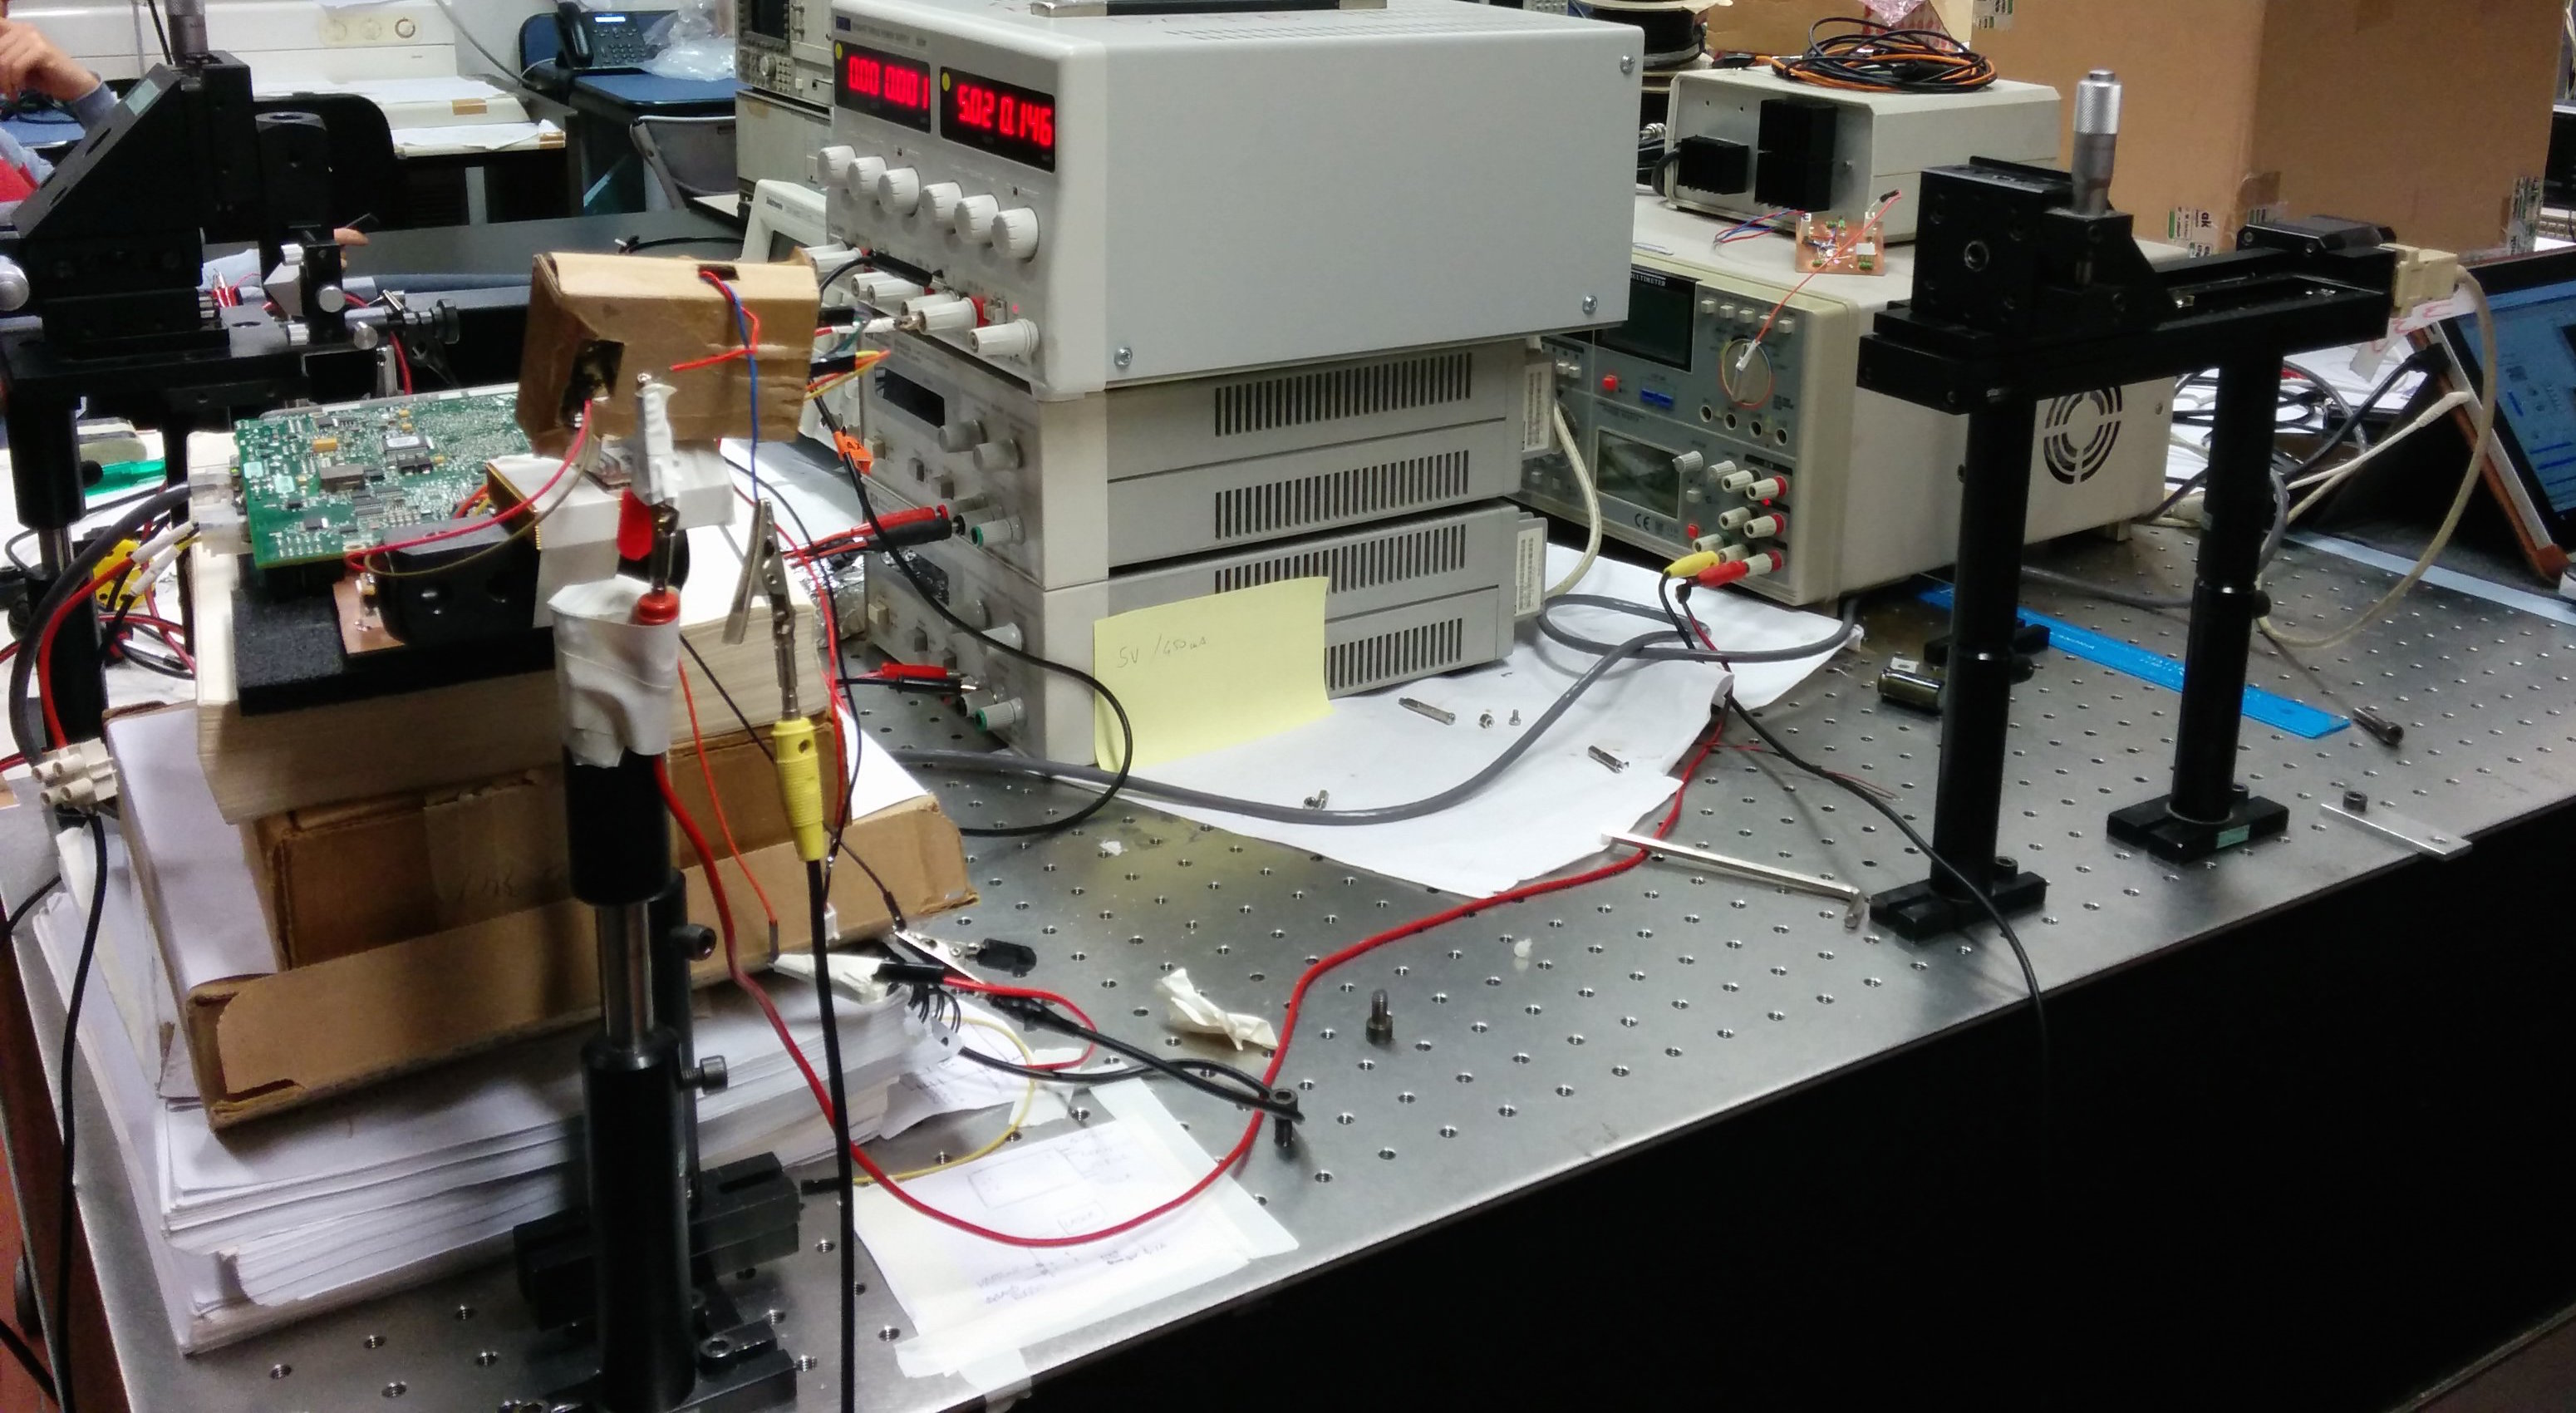
\includegraphics[scale=0.1]{cap5/allestimento}
    \caption{Allestimento della misura}
  \end{center}
\end{figure}

\subsection{Prova a bersaglio fisso}
La misura a bersaglio fisso è stata effettuata con il sensore fissato su di un tavolo ottico e puntato verso un bersaglio metallico nero, anch'esso fissato ad un tavolo ottico. L'uso del tavolo ottico si è reso necessario per minimizzare l'effetto delle vibrazioni.

Inizialmente si è lasciato in esecuzione il software che effettua la modulazione del laser, in modo da consentire al sensore di raggiungere una temperatura stabile, per minimizzare l'influenza del cambiamento di temperatura del laser sulla misura. Si è deciso di lasciare attiva la modulazione senza acquisire dati per circa $10$ minuti.

Con lo strumento ad una temperatura stabile si sono acquisiti $1000$ campioni della distanza dal bersaglio e se ne è valutata la media e la deviazione standard relativa. In questo modo è stato possibile valutare quanto è ampia l'oscillazione della misura rispetto alla media, e di determinare così la precisione dello strumento.

La misura si ritiene più precisa tanto minore è la sua deviazione standard relativa.

\subsection{Prova a bersaglio mobile}
La misura a bersaglio mobile è stata effettuata con un allestimento simile alla prova precedente. L'unica differenza è stato il fissaggio del bersaglio ad una slitta micrometrica, codice prodotto \textit{STANDA 8MT175-150}, uno strumento in grado di eseguire spostamenti dell'ordine dei micrometri, con una precisione di $0.31 \mu m$ \cite{standa}.

La prova si articola in due fasi:
\begin{enumerate}
	\item Acquisizione
	\item Spostamento
\end{enumerate}
Nella fase di acquisizione, con il bersaglio fermo, si acquisiscono $100$ campioni della distanza dal sensore. Di questi campioni si valutano media e deviazione standard relativa.
Nella fase di spostamento si allontana la slitta di $200 \mu m$ dal sensore. Si è scelto di utilizzare un passo di $200 \mu m$ perché consistente con la risoluzione dello strumento verificata nella prova a bersaglio fisso.

Queste due fasi sono ripetute per $15 \div 20$ volte, in modo da coprire una distanza totale di $3 \div 4 mm$.

Lo scopo della prova è quello di valutare la linearità dello strumento rispetto allo spostamento del bersaglio. Per fare questo si valuta l'oscillazione della misura rispetto alla retta ideale dello spostamento; in particolare si valutano distanza picco-picco dell'errore della misura rispetto alla retta ideale e l'RMS (\textit{Root Mean Square}, valore quadratico medio).

L'errore di misura è calcolato in modo semplice con la relazione:
\begin{equation}
	e = x_t - x 
\end{equation}
Dove con $x_t$ si intende il punto teorico appartenente alla retta ideale del valor medio, e con $x$ si intende il punto misurato dal sensore. 

La distanza picco-picco dell'errore è misurata come:
\begin{equation}
	e_{pp} = max(e) - min(e)
\end{equation}

I risultati migliori si ottengono quando si riscontrano distanze picco-picco ed RMS minori.

\subsection{Prova del range di misura}
La prova del range di misura si effettua con un allestimento identico alla prima prova, ma, al contrario di quest'ultima, i campioni acquisiti sono in numero minore, ovvero $100$. Il numero è stato scelto in modo coerente con il numero di campioni che lo strumento finale utilizzerà per fornire all'utente un singolo valore di distanza. 

Poiché lo scopo della prova è valutare il range di distanze in cui lo strumento è in grado di lavorare nei limiti di precisione desiderati, si ripete l'acquisizione dei campioni a diverse distanze dal sensore, partendo da $10 cm$ e arrivando a $100 cm$, con passi di $10 cm$ circa.

Sui $100$ campioni acquisiti si valutano media e deviazione standard relativa, e si ritiene soddisfacente la prestazione dello strumento quando la deviazione standard relativa fornita è minore di $10^{-3}$.

\section{Finestratura del segnale}
Come già discusso nel Capitolo \ref{capitolo4}, l'implementazione finale dello strumento genera un'onda triangolare che modula la sorgente laser in corrente.
\begin{figure}[H]
	\begin{center}
		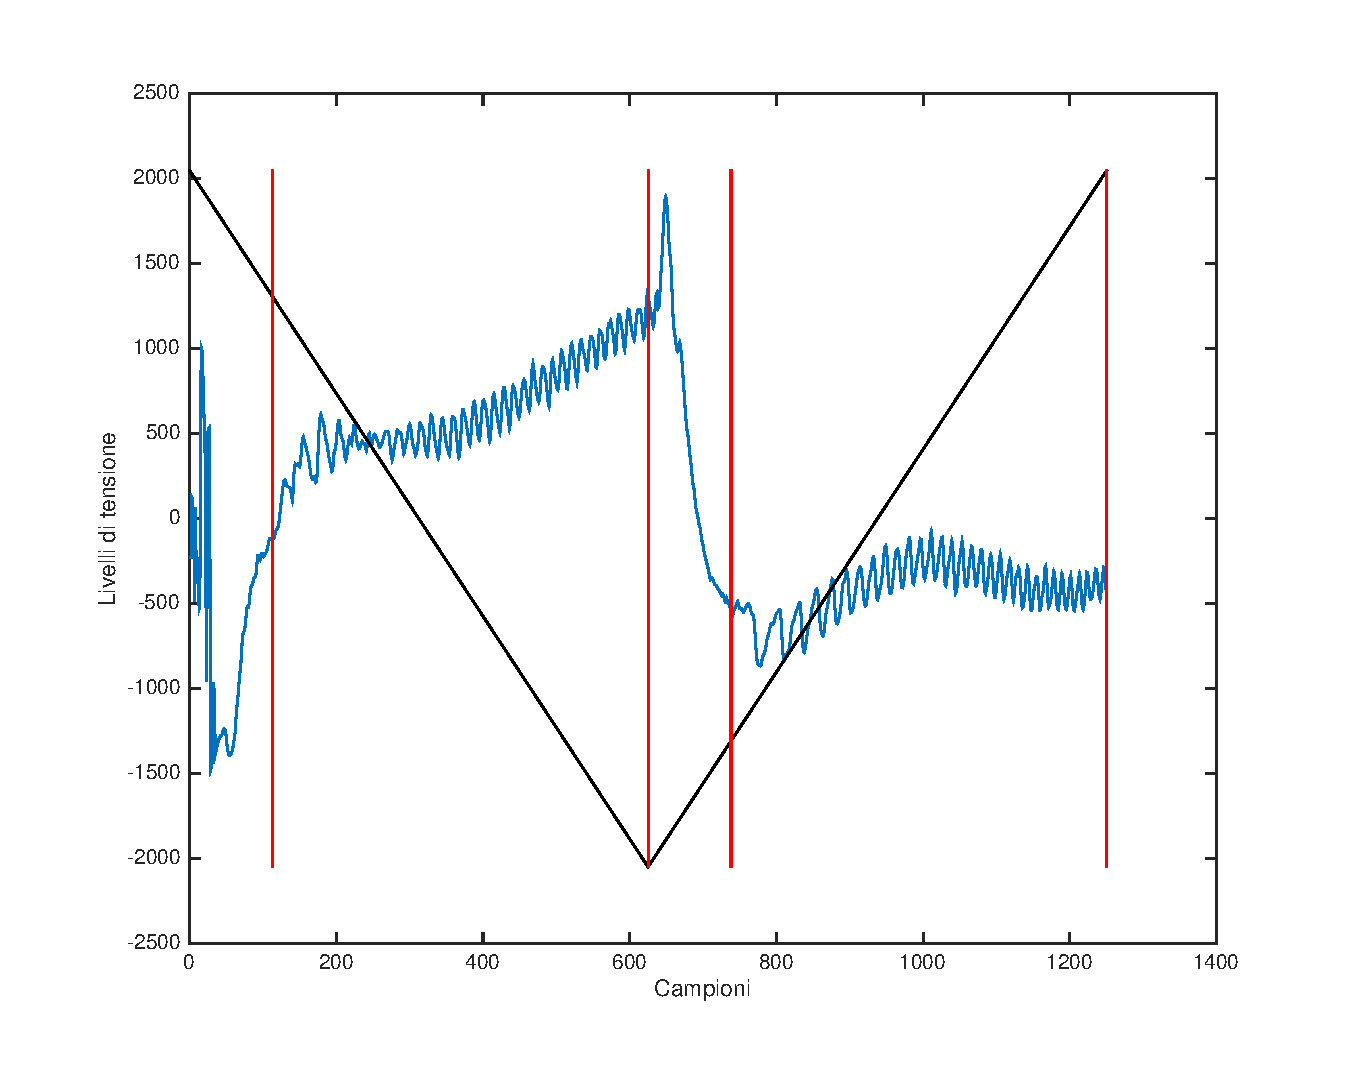
\includegraphics[scale=0.5]{cap5/segnaleinterf}
		\caption{Segnale interferometrico (blu) in un periodo di modulazione (nero)}
		\label{segnaleinterf}
	\end{center}
\end{figure}

L'onda di modulazione triangolare generata e il segnale interferometrico in risposta dal laser, sono formati entrambi da $1250$ punti, $625$ per il semiperiodo di discesa della triangolare di modulazione e $625$ per il semiperiodo di salita. 

Di questi $625$ punti soltanto $512$ contengono l'informazione utile per l'estrazione della frequenza interferometrica, poiché inizialmente si ha una parte di segnale influenzata dall'inversione del verso di polarizzazione del laser (Figura \ref{segnaleinterf}). 

Per l'estrazione del tono fondamentale del segnale si utilizza l'algoritmo di FFT interpolata a due punti con finestratura a $512$ punti.

Come accennato nel capitolo precedente, sono state valutate due differenti finestrature per il segnale: la finestra rettangolare e quella di \textit{Hanning}.

Per determinare quale delle due finestrature utilizzare nell'implementazione finale dello strumento sono state realizzate prove a bersaglio fisso e a bersaglio mobile con modulazione triangolare a pendenza fissa.
\begin{figure}[H]
\centering
\subfigure[Misure di distanza e media]
{\label{misfisso1a}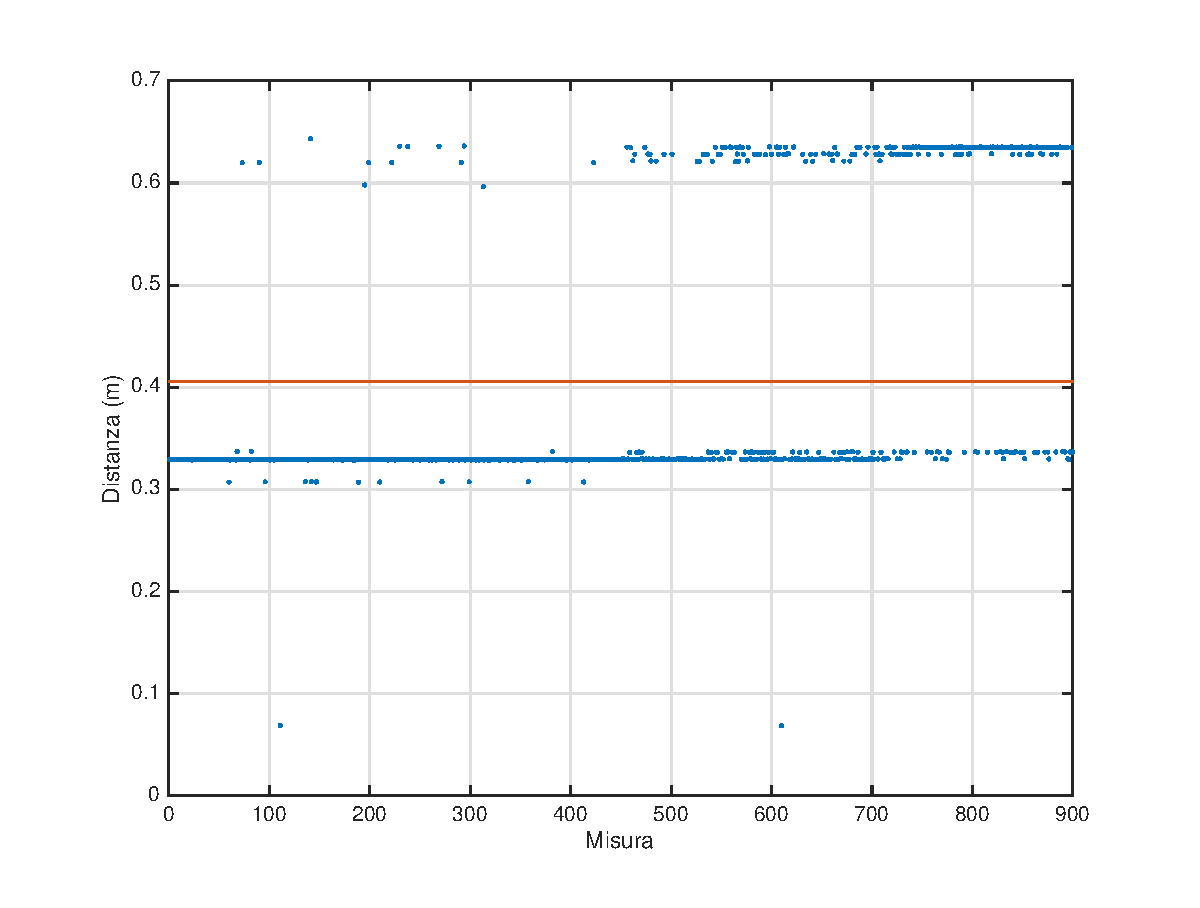
\includegraphics[scale=.5]{cap5/misfisso1a}}
\end{figure}
\begin{figure}[H]
\centering
\subfigure[Distribuzione dei valori misurati rispetto alla media]
{\label{misfisso1b}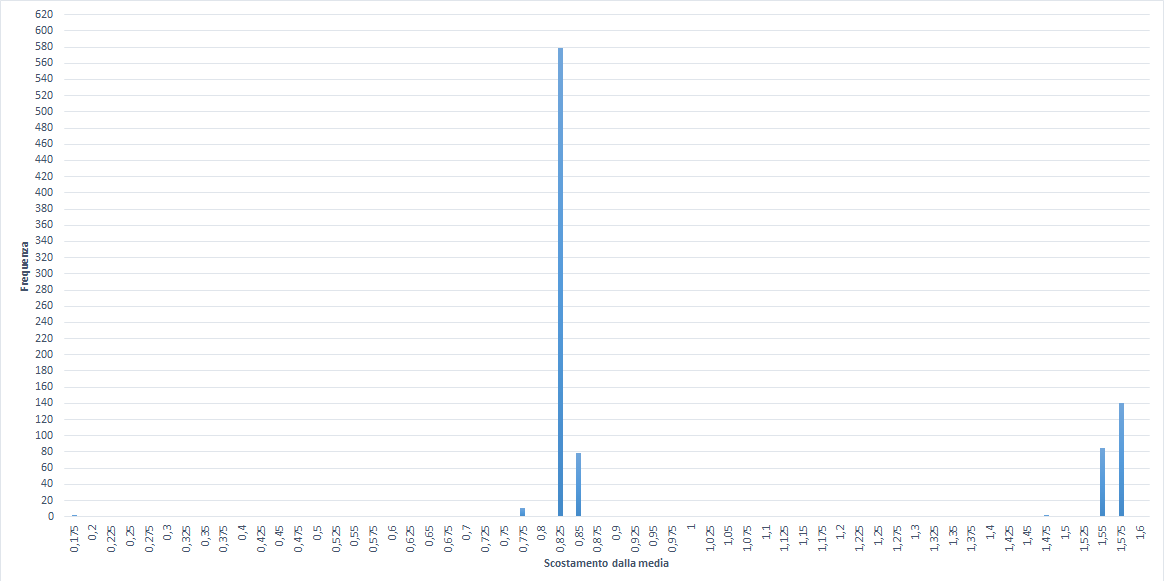
\includegraphics[scale=.4]{cap5/misfisso1b}}
\caption{Misure a bersaglio fisso con finestratura rettangolare}\label{misfisso1}
\end{figure}
\begin{figure}[H]
\centering
\subfigure[Misure di distanza e media]
{\label{misfisso2a}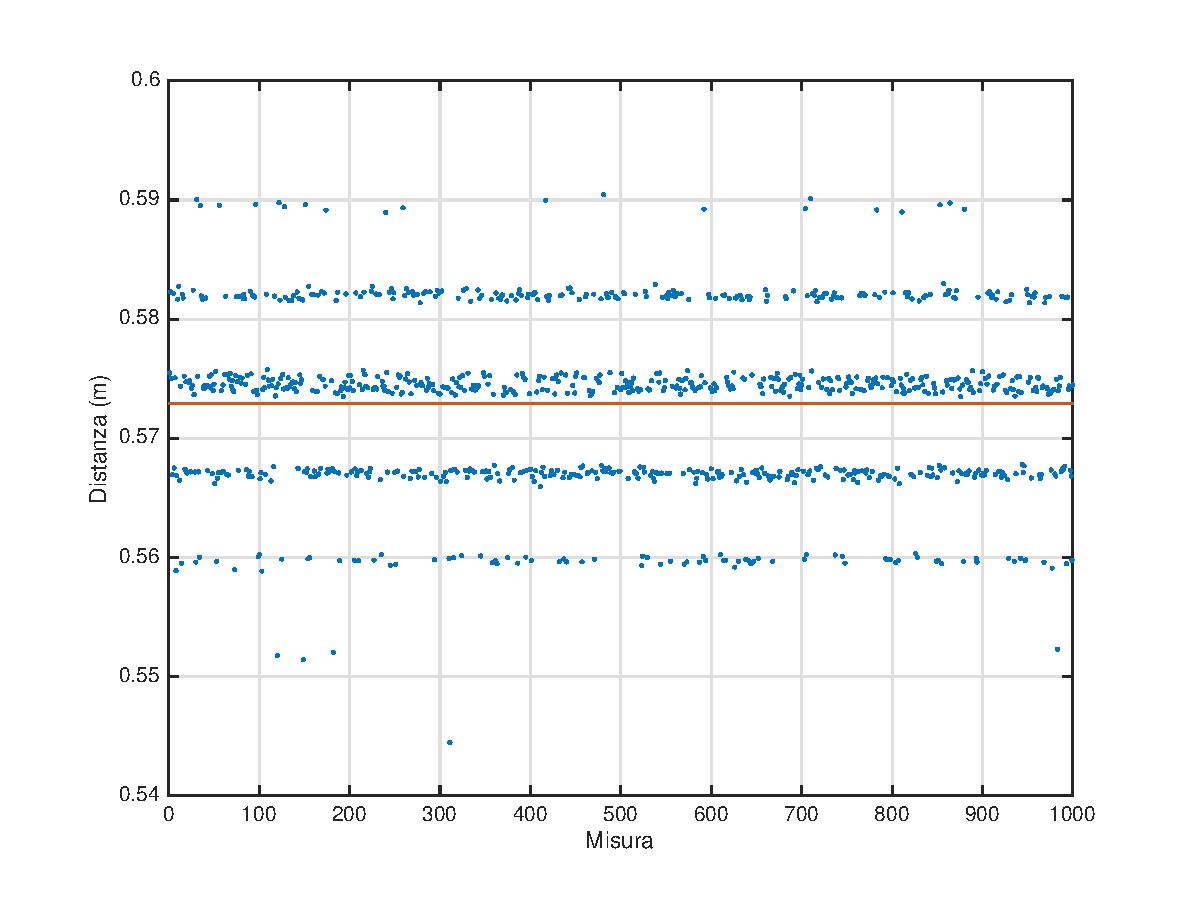
\includegraphics[scale=.5]{cap5/misfisso2a}}
\end{figure}
\begin{figure}[H]
\centering
\subfigure[Distribuzione dei valori misurati rispetto alla media]
{\label{misfisso2b}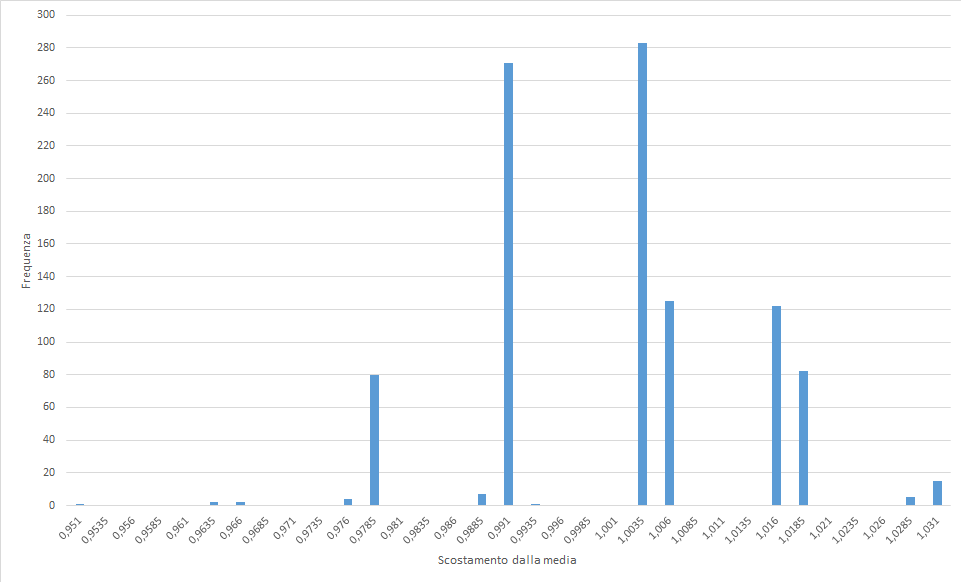
\includegraphics[scale=.5]{cap5/misfisso2b}}
\caption{Misure a bersaglio fisso con finestratura di Hanning}\label{misfisso2}
\end{figure}

\begin{figure}[H]
\centering
\subfigure[con finestra rettangolare]
{\label{mismobile1}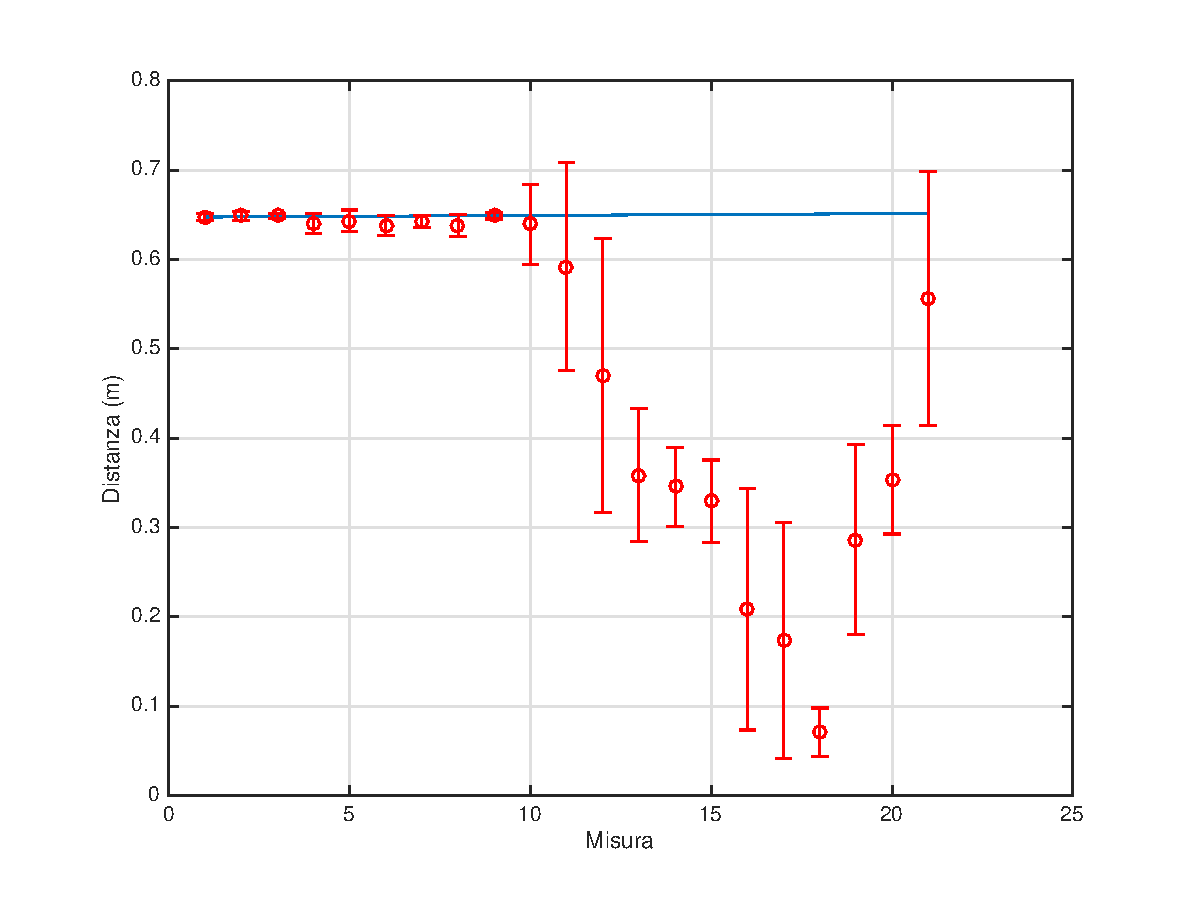
\includegraphics[scale=.5]{cap5/mismobile1}}
\end{figure}
\begin{figure}[H]
\centering
\subfigure[con finestra di Hanning]
{\label{mismobile2}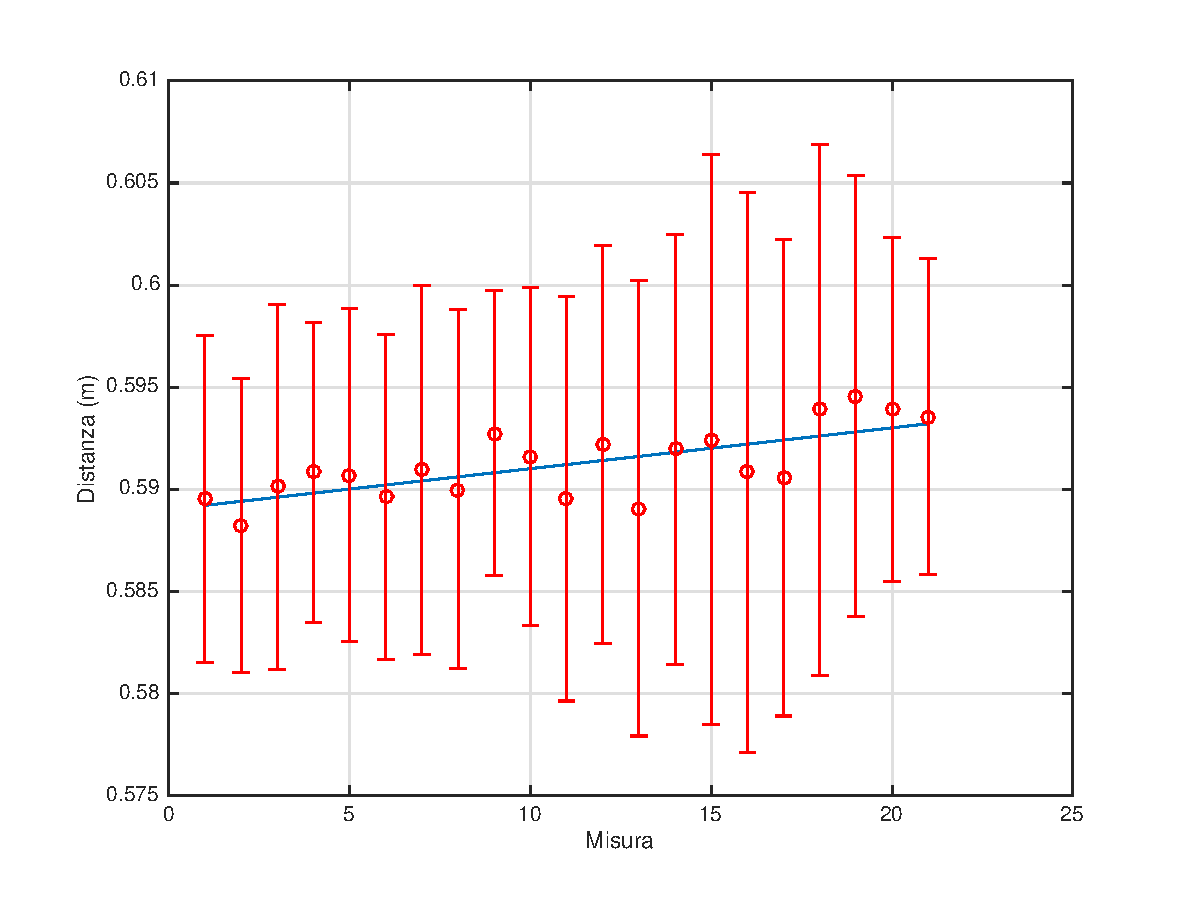
\includegraphics[scale=.5]{cap5/mismobile2}}
\caption{Misure di distanza a bersaglio mobile effettuate su $200 \mu m$ di spostamento}\label{mismobile12}
\end{figure}

I risultati delle prove a bersaglio fisso sono mostrati in Figura \ref{misfisso1} e \ref{misfisso2}. Sono inoltre riportati i grafici della distribuzione dei punti misurati rispetto alla media. In Figura \ref{mismobile12}, invece, sono mostrate le misure a bersaglio mobile: i punti rossi rappresentano le medie valutate ogni $100$ misurazioni, e le barre di errore mostrano l'incertezza assoluta di misura. La curva blu, invece, rappresenta il valore atteso.

Dai risultati delle misure a bersaglio fisso si evince che con la finestratura di \textit{Hanning} vi è un chiaro miglioramento in termini di precisione. L'incertezza relativa di misura si riduce complessivamente di un fattore $10$ passando da $10^{-1}$, con finestra rettangolare, a $10^{-2}$ con finestra di \textit{Hanning}.

Si nota inoltre, dai risultati delle misure a bersaglio mobile, che l'utilizzo della finestra di \textit{Hanning} rende lo strumento lineare allo spostamento con un errore massimo picco-picco dell'ordine del millimetro (ca. $4mm$). \'E facile intuire graficamente che l'utilizzo della finestra rettangolare rende lo strumento fortemente non lineare allo spostamento.
\begin{figure}  
  \begin{center}
    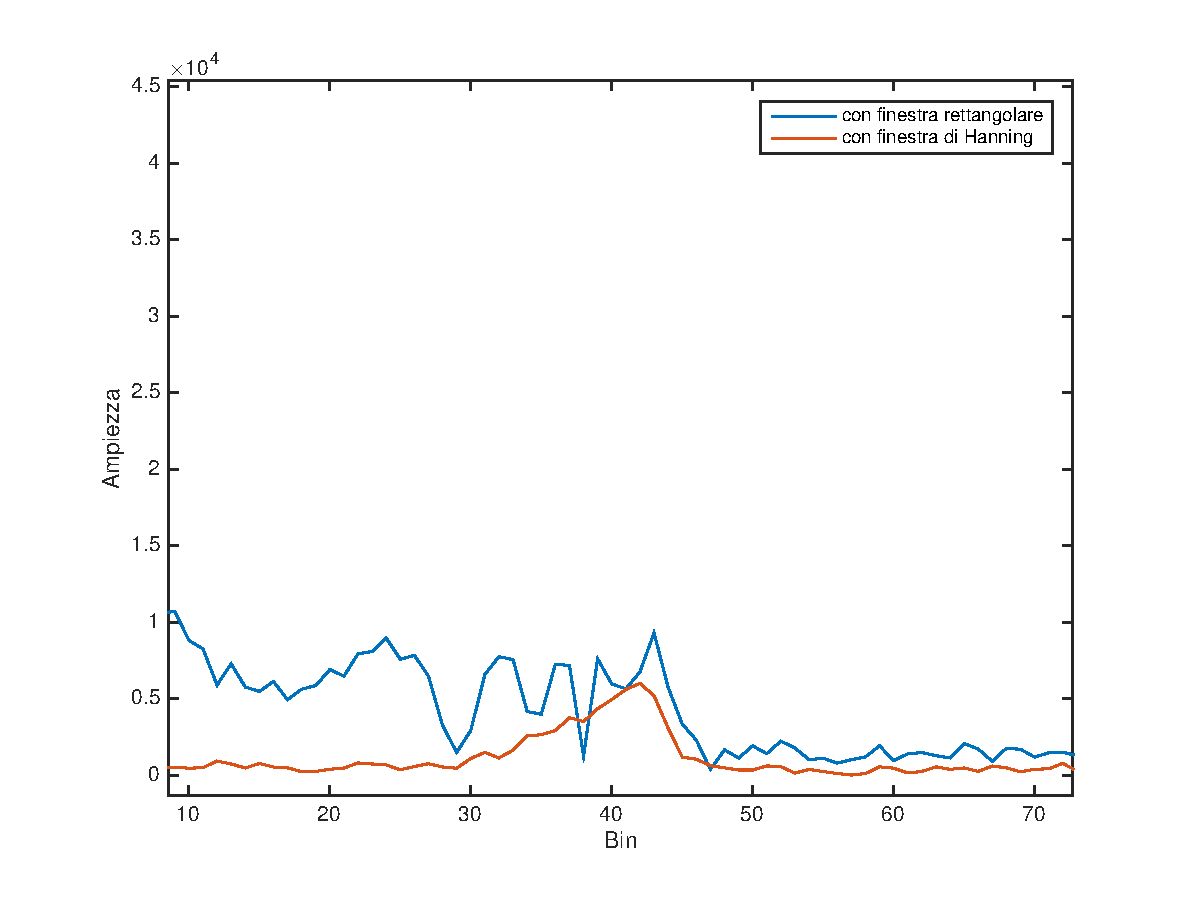
\includegraphics[scale=0.5]{cap5/spectleakinterf}
    \caption{Porzione di spettro calcolato sul fronte di discesa dalla FFT con finestra rettangolare e di Hanning}
    \label{spectleakinterf}
  \end{center}
\end{figure}

Il motivo che spiega questo miglioramento è la diminuzione dello \textit{spectral leakage}, che risulta meno marcato per la finestra di \textit{Hanning} piuttosto che per quella rettangolare. In Figura \ref{spectleakinterf} sono confrontati gli spettri di frequenza di un segnale interferometrico calcolati sul fronte di discesa dalla FFT con finestra rettangolare e di \textit{Hanning}. Dalla figura si nota l'evidente effetto dello \textit{spectral leakage} che affligge la FFT con finestra rettangolare.

\section{Linearizzazione della misura}
Nonostante i notevoli miglioramenti in termini di precisione, il misuratore possiede ancora una scarsa accuratezza. Tale limitazione dipende dalla lunghezza del periodo di frangia del segnale interferometrico. In particolare, fissata la distanza $s$ dell'ostacolo e modulando triangolarmente il laser, quindi con pendenza $\frac{\Delta I}{\Delta t}$ costante, il periodo di frangia $t_{frangia}$ dovrebbe essere costante lungo tutto il segnale. 

Tuttavia, come osservato in Figura \ref{semiperiodononcomp}, il periodo della singola frangia $t_{frangia}$ non è costante lungo tutto il fronte di salita o di discesa. Di conseguenza, questo fenomeno è la causa del limite sull'accuratezza della misura.

Questo limite sull'accuratezza è dovuto alla non-linearità del laser. \'E possibile notare dall'equazione utilizzata per il calcolo della distanza assoluta: 
\begin{equation}
	s = \frac{\lambda^2}{2\left ( \frac{\Delta I}{\Delta t} \frac{\Delta \lambda}{\Delta I} \right ) t_{frangia}} 
\end{equation}
che è il parametro $\chi = \frac{\Delta \lambda}{\Delta I}$ a causare la non-linearità del periodo di frangia. Infatti dal momento in cui tutti i parametri sono fissati, l'unico che può causare la non-linearità è appunto $\chi$.

Un secondo motivo per cui il tempo di frangia $t_{frangia}$ non è costante è la costante termica del laser, che causa un ritardo nel raggiungimento di una condizione di equilibrio.

Queste caratteristiche sono peculiari della sorgente, e sono esclusivamente dipendenti dalla frequenza di modulazione della corrente.	

I due effetti combinati, quindi, causano una non linearità nella frequenza delle frange; in particolare le frange che si trovano all'inizio del segnale interferometrico sono a frequenza più bassa di quelle alla fine.
\begin{figure}[H]
	\begin{center}
		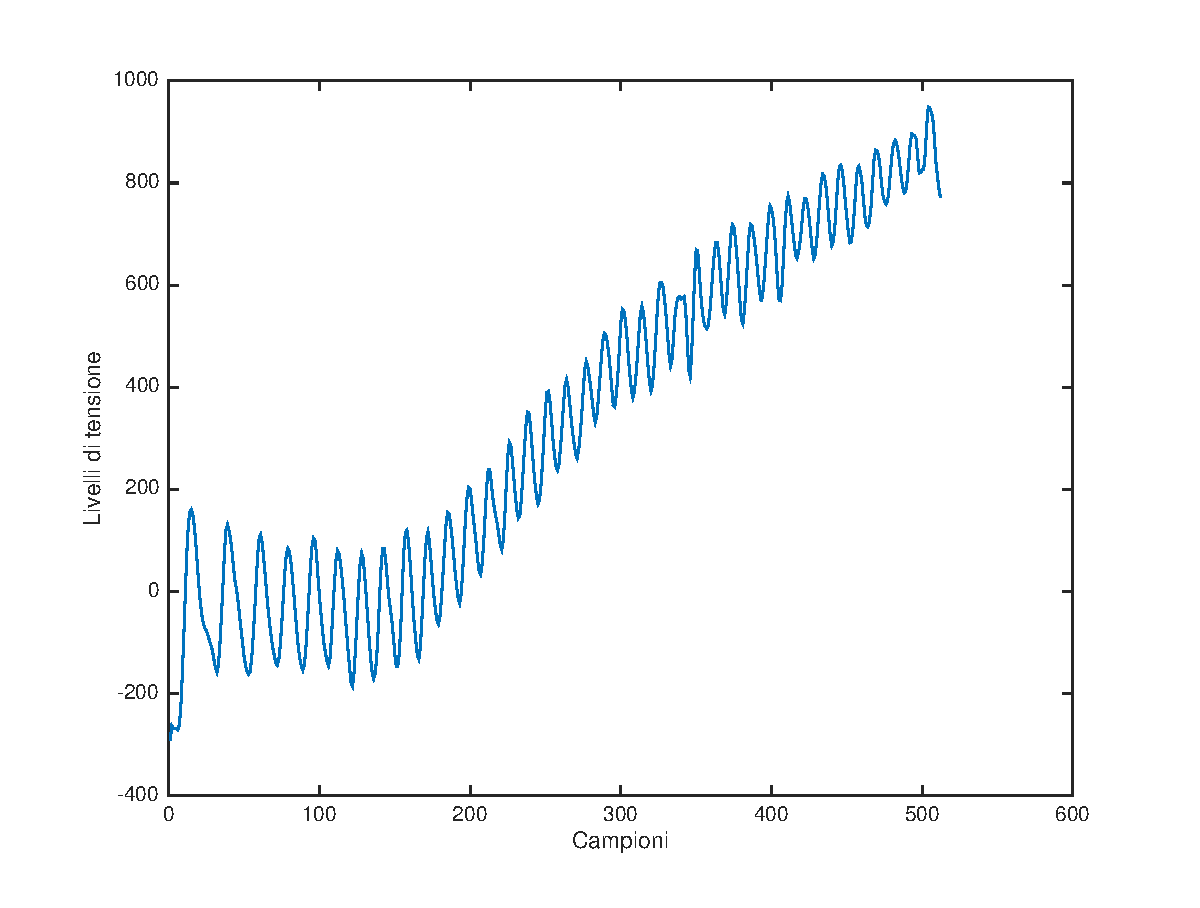
\includegraphics[scale=0.5]{cap5/semiperiodononcomp}
		\caption{Semiperiodo del segnale interferometrico prodotto dalla sorgente laser con modulazione a pendenza $\frac{\Delta I}{\Delta t}$ costante su di un bersaglio metallico a distanza fissa}
		\label{semiperiodononcomp}
	\end{center}
\end{figure}

\subsection{Metodo di compensazione della non-linearità}
\label{subsec:metodocomp}
Una tecnica per compensare le variazioni del parametro $\chi = \frac{\Delta \lambda}{\Delta I}$ consiste nell'utilizzare un segnale modulante con pendenza $\frac{\Delta I}{\Delta t}$ variabile durante il semiperiodo di modulazione. Per fare ciò è necessario ricavare l'andamento $\chi = \frac{\Delta \lambda}{\Delta I}$ conoscendo quello del $t_{frangia}$ o, in alternativa, $f_{frangia}$. Una volta ricavato l'andamento non-lineare nel tempo di $\chi = \frac{\Delta \lambda}{\Delta I}$ lo si compensa, modificando $\frac{\Delta I}{\Delta t}$, in modo che il prodotto $\frac{\Delta I}{\Delta t} \frac{\Delta \lambda}{\Delta I}$ sia costante e, di conseguenza, anche $t_{frangia}$ risulti costante.

Il metodo utilizzato per ricavare la forma d'onda del segnale di modulazione è stato implementato in LabVIEW Real-Time ed eseguito sul microprocessore della scheda di prototipazione. Per permettere ciò, è stato sviluppato un firmware FPGA, leggermente diverso de quello implementato nello strumento finale, che permettesse di inviare al microprocessore il segnale interferometrico completo e non solo i risultati dell'algoritmo di FFT.
\begin{figure}[H] 
	\begin{center}
		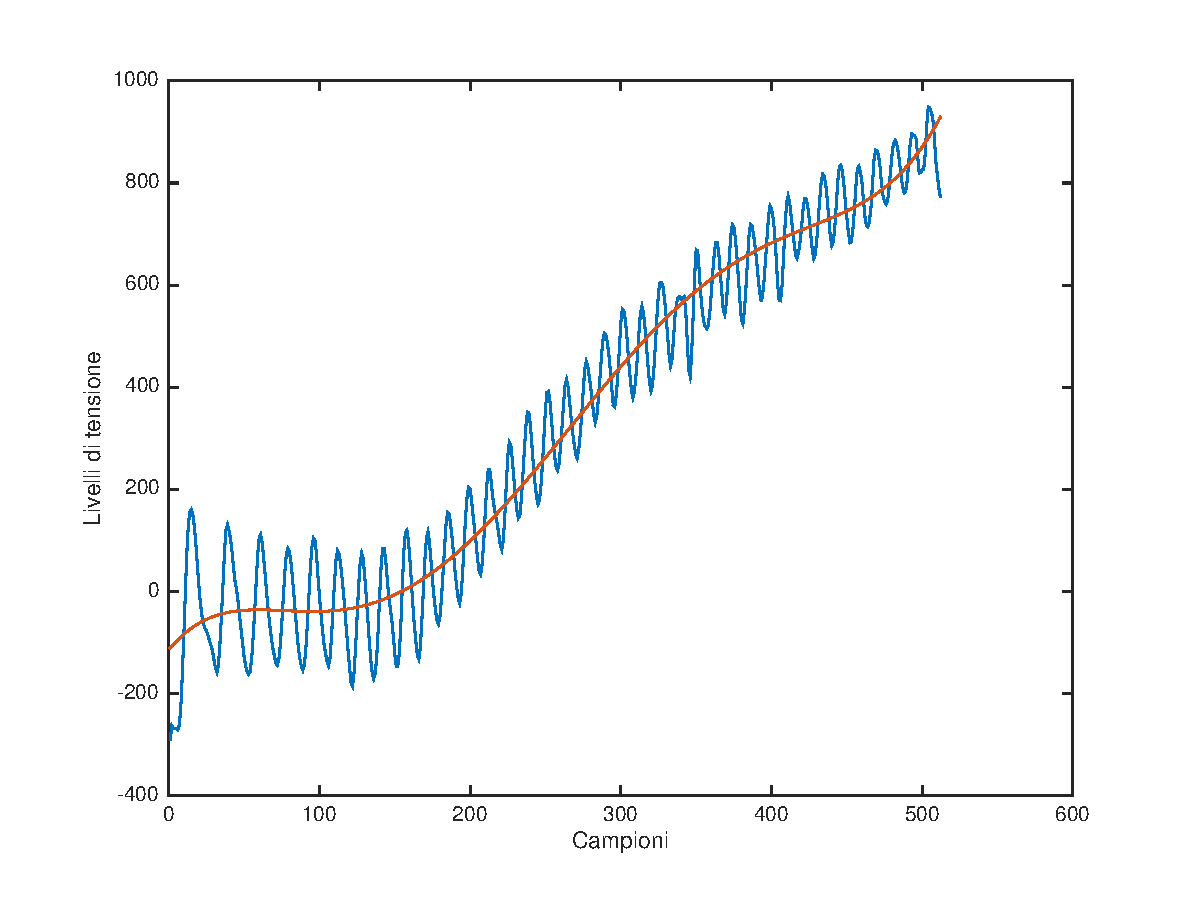
\includegraphics[scale=0.5]{cap5/regressioncurvefrangia}
		\caption{Curva di regressione polinomiale del segnale interferometrico}
		\label{regressioncurvefrangia}
	\end{center}
\end{figure}

Di seguito vengono descritti i passi principali del metodo di compensazione sviluppato:

\begin{enumerate}
	\item \underline{Modulazione triangolare}: La forma d'onda utilizzata per la modulazione è un'onda triangolare simmetrica con pendenza fissa. Il bersaglio è posto ad un distanza tale da produrre un elevato numero di frange (nel nostro caso si è posto il bersaglio a circa $50cm$ dal sensore).
	\item \underline{Calcolo della curva di regressione polinomiale}: Per avere una misura più precisa delle frequenza di frangia è stata calcolata la curva di regressione polinomiale di grado $5$ del segnale interferometrico (esempio in Figura \ref{regressioncurvefrangia}) ed è stata sottratta digitalmente da esso. In questo modo la lunghezza del tempo di frangia è valutata in modo più rigoroso.
	
	\item \underline{Calcolo della curva delle variazioni delle frequenze di frangia}: L'algoritmo analizza separatamente i due fronti, ricevendo in ingresso i $512$ campioni del segnale interferometrico per ciascun fronte. Per ogni fronte si selezionano i primi $128$ campioni e si estrae il valore di frequenza corrispondente alle prime frange del segnale. Per l'estrazione della frequenza del segnale, LabVIEW offre un metodo già implementato chiamato \textit{Extract Single Tone Information}. Si tratta di una FFT con finestra di \textit{Hanning} interpolata a due punti, con una correzione per l'aliasing intorno alla continua a $\frac{f_{sample}}{2}$. A questo punto la finestra di selezione viene traslata di un campione verso destra e la frequenza delle frange viene ricalcolata (Figura \ref{slidingfft}). Questa operazione viene effettuata fino a che la selezione comprende l'ultimo campione del segnale interferometrico.
	In questo modo si ottengono $384$ valori di frequenze per ciascun fronte, in funzione della posizione delle frange all'interno del fronte stesso (Figura \ref{curvamediatafreq}). Questo procedimento è stato effettuato per $100$ segnali acquisiti ed i risultati sono stati poi mediati. \'E stato deciso di associare ai primi $113$ ($=625-512$) campioni scartati valori di frequenza fittizi, approssimando tali valori con una retta di pendenza pari alla pendenza della prima frequenza estratta, mentre agli ultimi $128$ ($=512-384$) campioni è stata associata una retta con pendenza pari alla pendenza dell'ultima frequenza estratta.
		\begin{figure}[H]  
			\begin{center}
				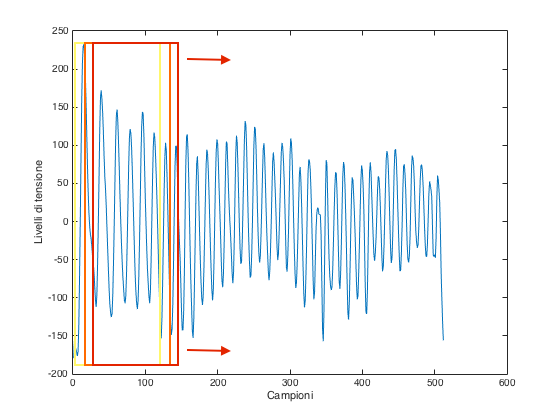
\includegraphics[scale=0.5]{cap5/slidingfft}
				\caption{Spostamento della finestra di 128 campioni lungo il semiperiodo di modulazione su cui viene calcolata la FFT}
				\label{slidingfft}
			\end{center}
		\end{figure}
		
		\begin{figure}[H]  
			\begin{center}
				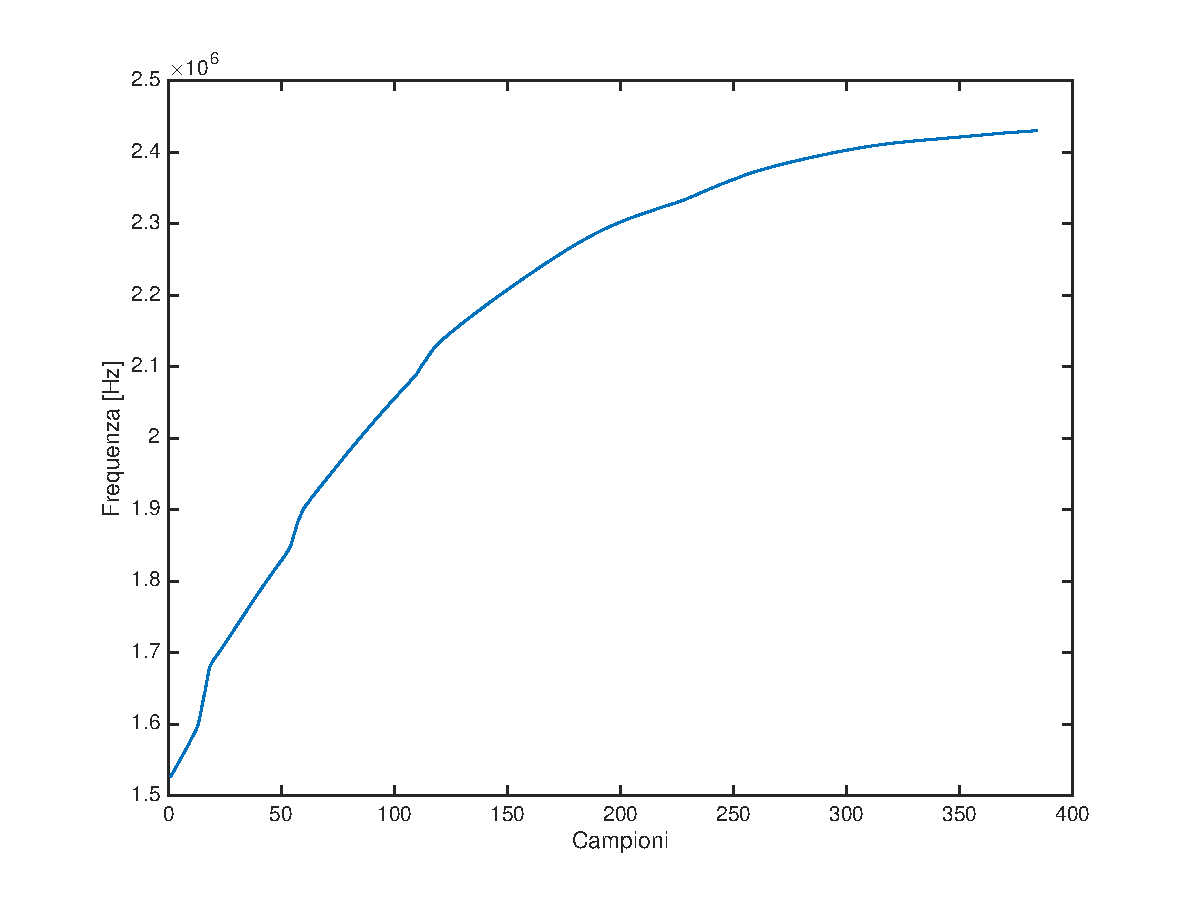
\includegraphics[scale=0.5]{cap5/curvamediatafreq}
				\caption{Curva mediata delle frequenze in un semiperiodo di modulazione con ostacolo a distanza fissa}
				\label{curvamediatafreq}
			\end{center}
		\end{figure}
		
	
	\item \underline{Calcolo iterativo del fattore moltiplicativo} \underline{da applicare alla curva delle} \underline{frequenze}: La curva mediata delle frequenze, ricavata al passo precedente, viene moltiplicata alla triangolare con pendenza costante ricavando così il segnale di modulazione con pendenza $\frac{\Delta I}{\Delta t}$ non costante.
	Da verifiche sperimentali è nata la necessità di moltiplicare i semiperiodi della curva di modulazione per un fattore di scala, che è stato scelto in modo che la deviazione standard relativa delle frequenze rilevate dall'FFT a scorrimento sia la minore possibile.	
	Questo fattore viene ricavato iterativamente. Partendo da un valore $1$ e diminuendo il fattore di scala di passi di $0.1$ fino ad arrivare a $0$, si calcola la deviazione standard relativa delle frequenze estratte dall'FFT a scorrimento e si sceglie il fattore di scala che la minimizza.	
	Questo procedimento è stato reiterato una seconda volta aumentando il numero di cifre significative del fattore di scala stesso (partendo da $0.35$ ed arrivando a $0.15$ con passi di $0.01$), in modo da aumentare la precisione della linearizzazione.	
	Le prime curve ricavate vengono presentate in Figura \ref{mulfact}. Si può notare che sia per il fronte di salita che per il fronte di discesa il minimo si trova nell'intorno di $0.2$. I valori esatti ricavati nella seconda iterazione sono $0.18$ per il fronte di discesa e $0.22$ per il fronte di salita.
		\begin{figure}[H]
			\centering
			\subfigure[Semiperiodo di discesa]
			{\label{}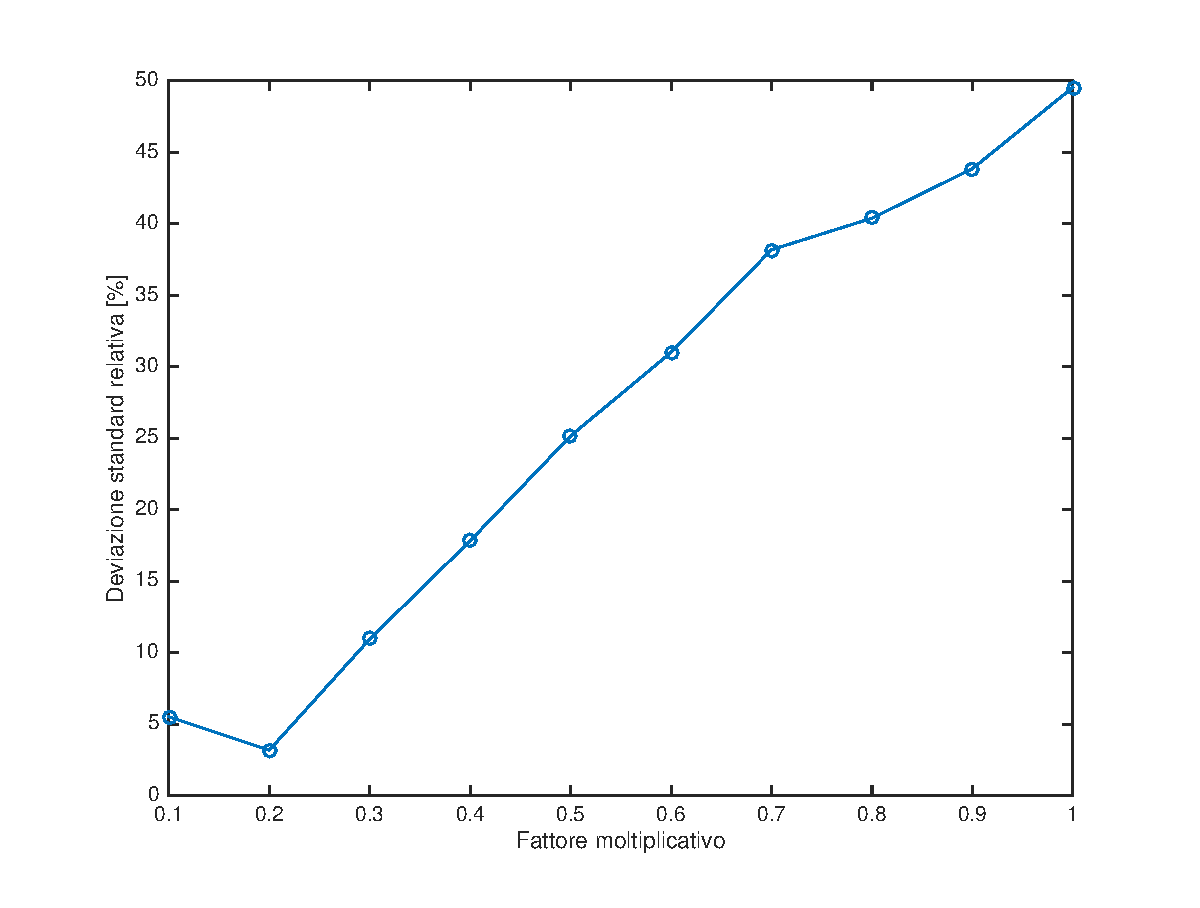
\includegraphics[scale=.5]{cap5/mulfactdiscesa}}
		\end{figure}
		\begin{figure}[H]
			\centering
			\subfigure[Semiperiodo di salita]
			{\label{}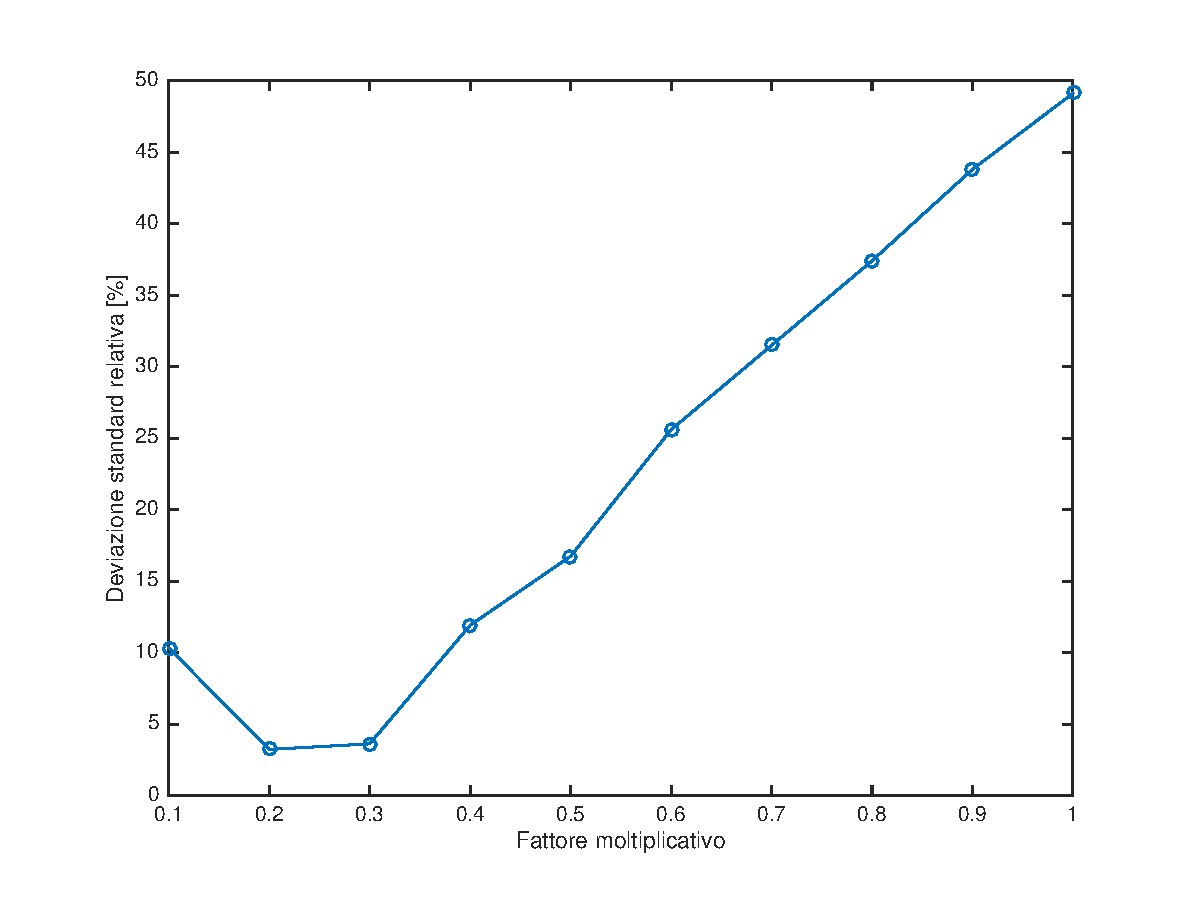
\includegraphics[scale=.5]{cap5/mulfactsalita}}
			\caption{Curva delle deviazioni standard relative dei due fronti al variare del fattore moltiplicativo}\label{mulfact}
		\end{figure}
	
	\item \underline{Generazione della curva di modulazione compensata}: Le curve delle variazioni delle frequenze di frangia, calcolate al passo 2, vengono scalate dei valori moltiplicativi calcolati al passo precedente. Le curve scalate vengono poi moltiplicate ai semiperiodi della triangolare con pendenza costante ricavando così il segnale di modulazione con pendenza $\frac{\Delta I}{\Delta t}$ non costante.
    \begin{figure}[H]
    	\begin{center}
    		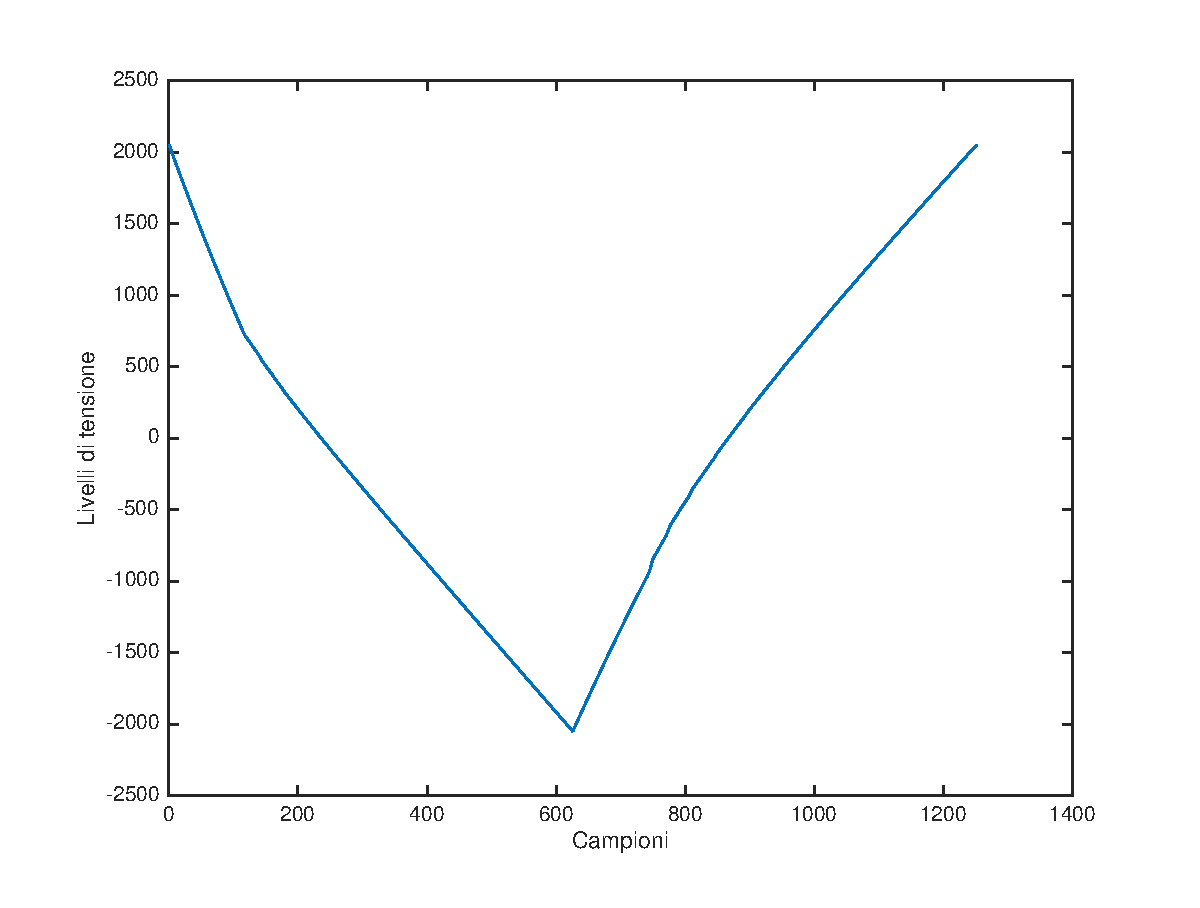
\includegraphics[scale=0.6]{cap5/ondafinale}
    		\caption{Forma d'onda finale usata per la modulazione}
    		\label{ondafinale}
    	\end{center}
    \end{figure}
		
\end{enumerate}

La forma d'onda finale, mostrata in Figura \ref{ondafinale}, ha consentito di ridurre la dispersione del $t_{frangia}$, migliorando l'accuratezza della misura di distanza. La pendenza iniziale sia nel fronte di salita che in quello di discesa è accentuata rispetto alla triangolare originaria, come era prevedibile dallo studio in frequenza. Infatti la frequenza di frangia presentava un andamento monotono crescente al variare della corrente di modulazione, effetto compensato dall'aumento della pendenza nella triangolare compensata.

\subsection{Misure in seguito alla compensazione}
Al fine di valutare la bontà dell'algoritmo precedentemente descritto, è stata comparata quantitativamente l'incertezza relativa della variazione di frequenza del segnale interferometrico prima e dopo la compensazione del segnale di modulazione.

\begin{figure}[H]
\centering
\subfigure[Semiperiodo di discesa]
{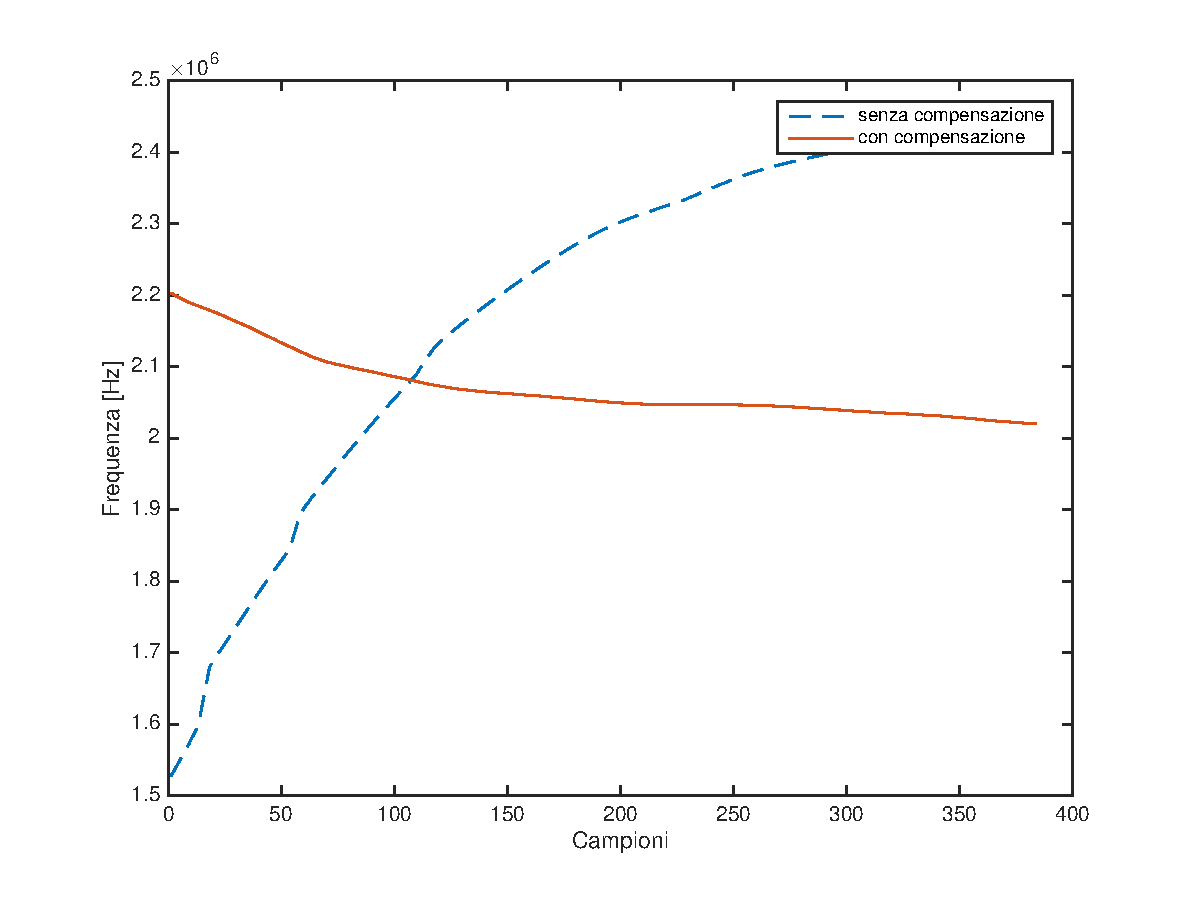
\includegraphics[scale=.5]{cap5/primadopocompdisc}}
\end{figure}
\begin{figure}[H]
\centering
\subfigure[Semiperiodo di salita]
{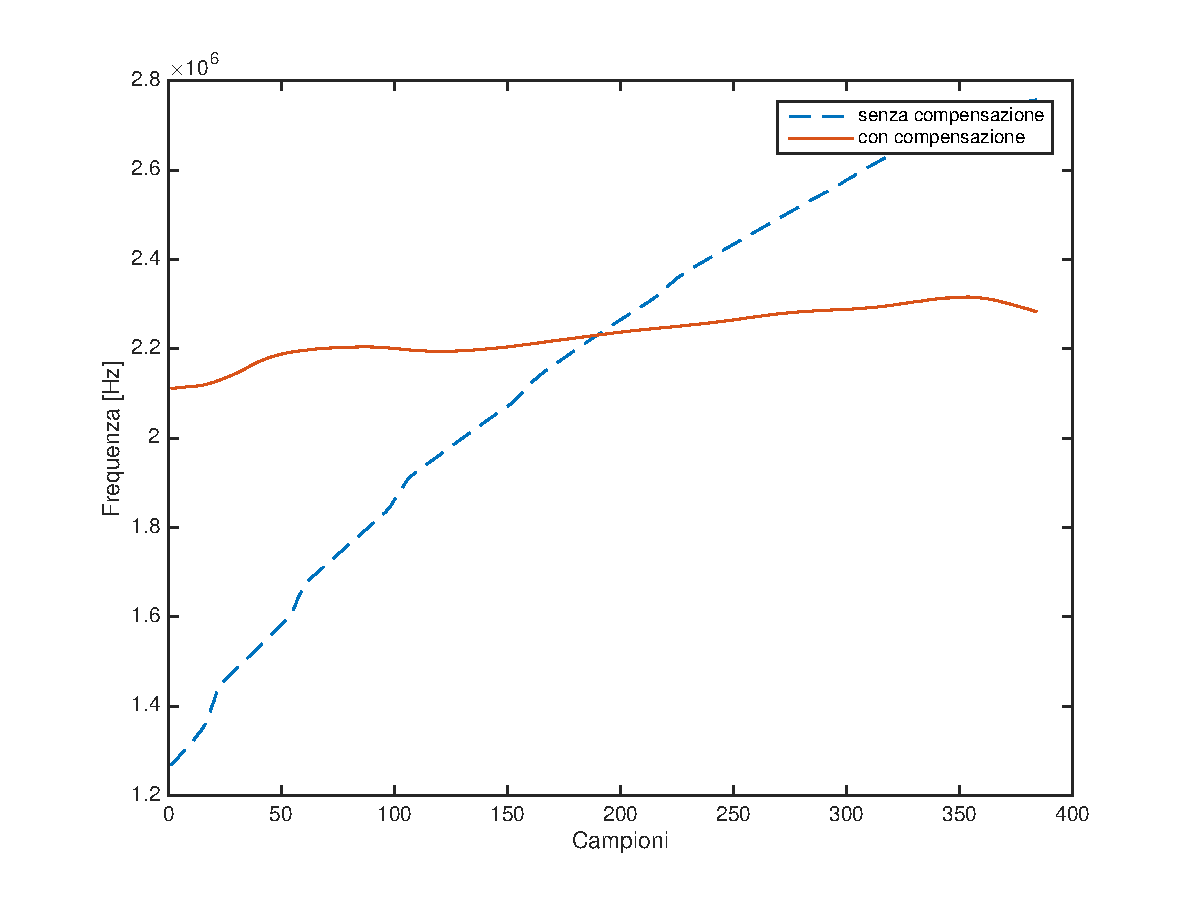
\includegraphics[scale=.5]{cap5/primadopocompsal}}
\caption{Curve mediate delle frequenze estratte per entrambi i fronti di modulazione, prima e dopo la compensazione}\label{primadopocomp}
\end{figure}

I miglioramenti ottenuti per merito della compensazione della non-linearità sono mostrati in Figura \ref{primadopocomp}. Dalle prove sperimentali è emerso che l'incertezza relativa della variazione di frequenza, valutata su $100$ semiperiodi di modulazione, è scesa intorno al $2\%$, per entrambi i fronti di modulazione, contro i $20\%$ ottenuti senza compensazione. La prova è stata ripetuta più volte per verificare che il guadagno in termini di linearità del periodo di frangia sia effettivamente $10$.

Questo miglioramento ha influito sulla precisione e sull'accuratezza della misura. A conferma del risultato sono riportati gli esiti delle prove a bersaglio fisso e a bersaglio mobile rispettivamente in Figura \ref{misfisso3} e \ref{mismobile3}.

Si può apprezzare, dai risultati delle misure a bersaglio fisso, che utilizzando un segnale di modulazione compensato la precisione di misura migliora sensibilmente. In particolare, l'incertezza relativa diminuisce di due ordini di grandezza, passando da $10^{-2}$ a $4 \cdot 10^{-4}$.

Inoltre, si può notare come le misure effettuate con la modulazione compensata risultino complessivamente più lineari rispetto a quelle effettuate senza compensazione.

La valutazione dell'errore massimo picco-picco rispetto al valore atteso conferma quanto intuito graficamente: l'errore nel caso di segnale di modulazione con pendenza compensata migliora considerevolmente passando da $4mm$ a $826 \mu m$, con un RMS pari a $568 \mu m$.

Nonostante l'ottimo miglioramento raggiunto, l'accuratezza non è ancora soddisfacente, a tal proposito si è ritenuto opportuno migliorare ulteriormente la misura con ottimizzazioni che verranno descritte nel paragrafo successivo.
\begin{figure}[H]
	\centering
	\subfigure[Misure di distanza e media]
	{\label{misfisso3a}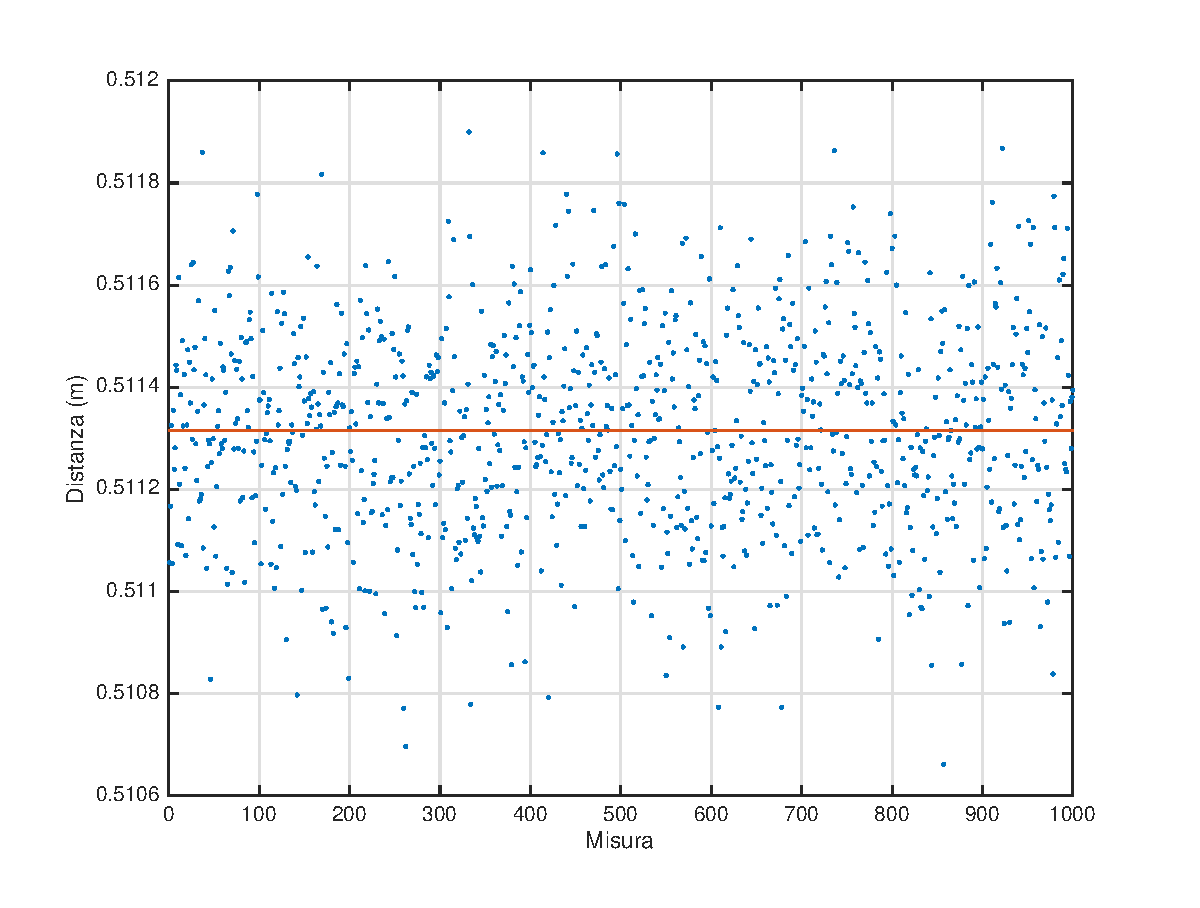
\includegraphics[scale=.5]{cap5/misfisso3a}}
\end{figure}
\begin{figure}[H]
	\centering
	\subfigure[Distribuzione dei valori misurati rispetto alla media]
	{\label{misfisso3b}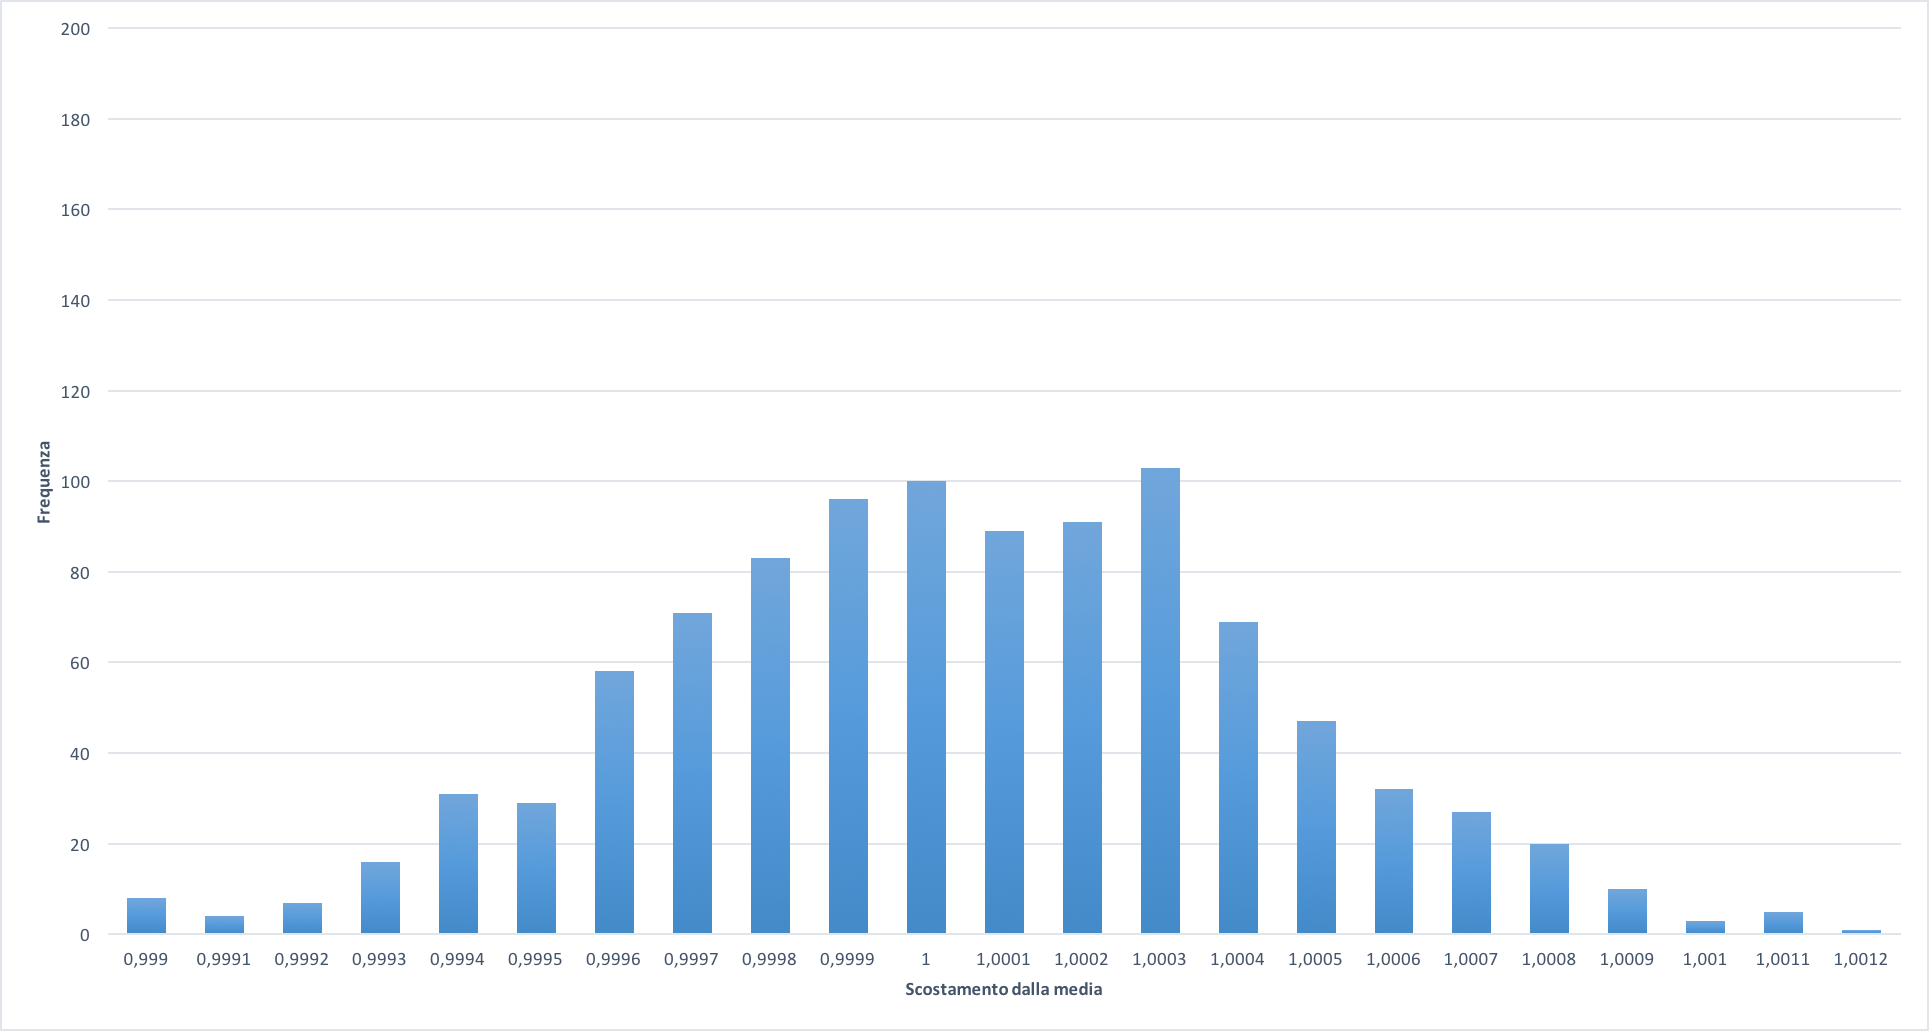
\includegraphics[scale=.4]{cap5/misfisso3b}}
	\caption{Misure a bersaglio fisso con segnale di modulazione compensato}\label{misfisso3}
\end{figure}

\begin{figure}[H]  
	\begin{center}
		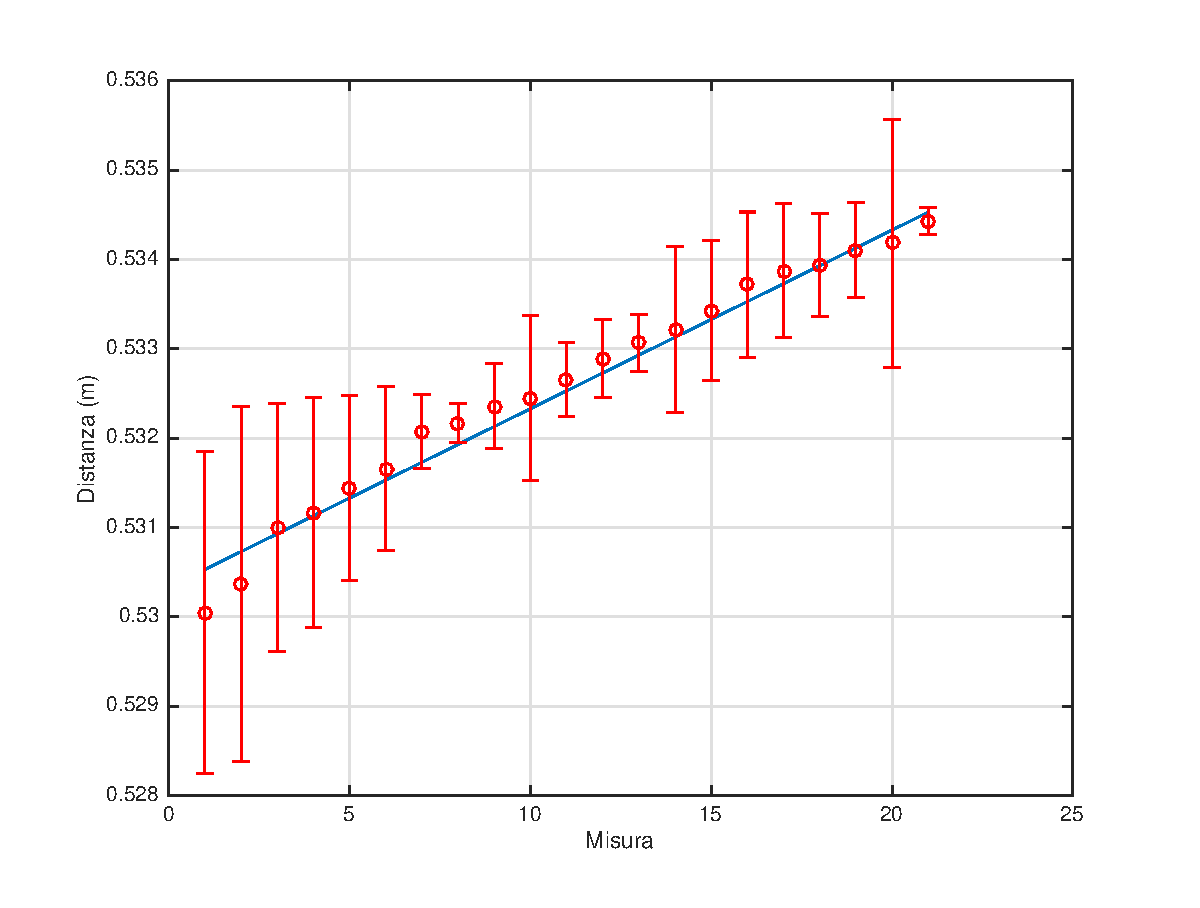
\includegraphics[scale=0.5]{cap5/mismobile3}
		\caption{Misure di distanza a bersaglio mobile effettuate su $200\mu m$ di spostamento con segnale di modulazione compensato}
		\label{mismobile3}
	\end{center}
\end{figure}

\section{Ottimizzazione della misura}
In questo paragrafo verranno discusse le ottimizzazioni sviluppate al fine di migliorare la precisione e l'accuratezza della misura.

\subsection{Variazione dell'ampiezza del segnale di modulazione}
\begin{figure}[H]
  \begin{center}
    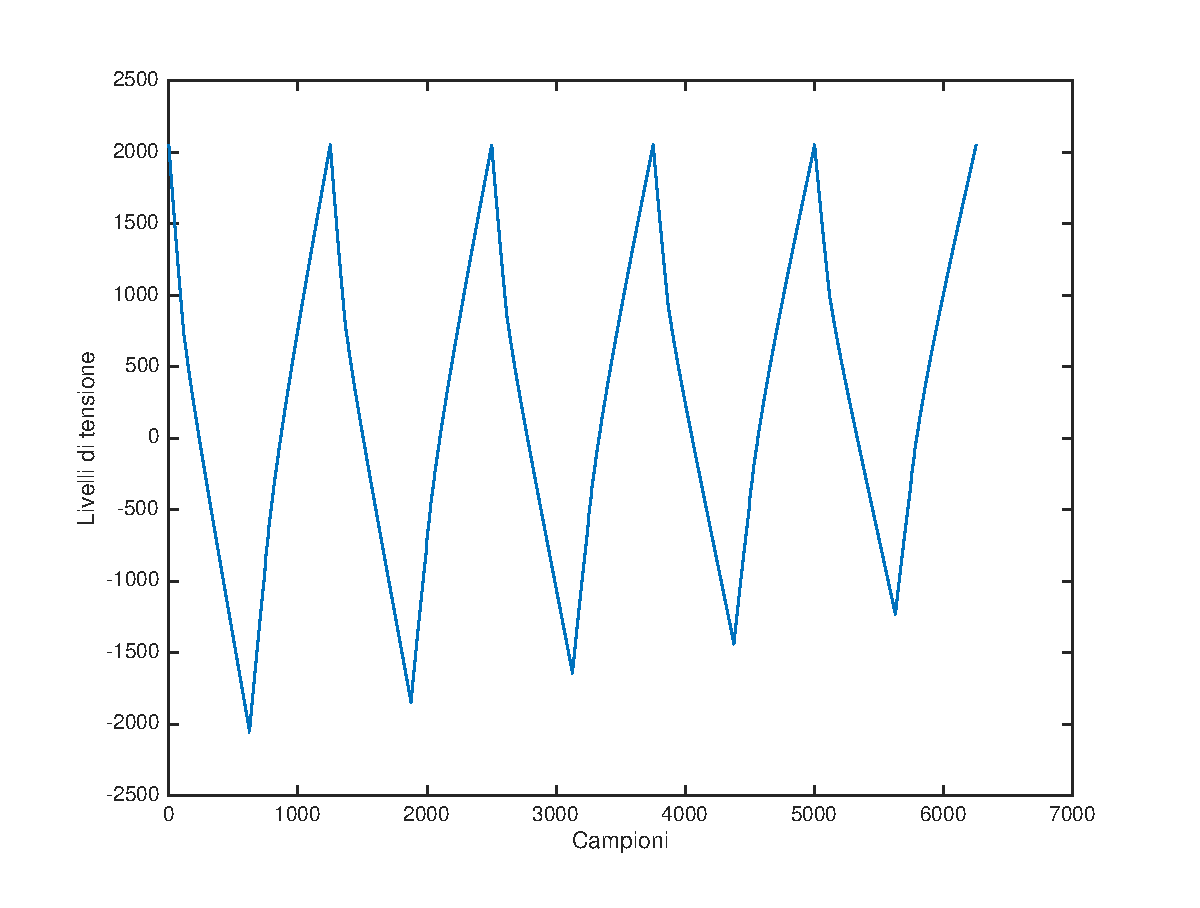
\includegraphics[scale=0.5]{cap5/cinquesegnali}
    \caption{Segnale di modulazione compensato, costituito da cinque forme d'onda di ampiezza diversa}
    \label{cinquesegnali}
  \end{center}
\end{figure}

Per cercare di mitigare effetti dipendenti dall'ampiezza del segnale di modulazione sul laser si è deciso di utilizzare un segnale di modulazione ad ampiezza variabile. Poiché le prestazioni dello strumento in termini di velocità di acquisizione di una singola misura sono piuttosto elevate (il tempo di misura teorico è di circa $40 \mu s$), si è deciso di utilizzare $5$ segnali di modulazione con ampiezze differenti (Figura \ref{cinquesegnali}). Le ampiezze scelte per i segnali sono state rispettivamente di $100\%$, $95\%$, $90\%$, $85\%$ e $80\%$ rispetto al segnale di modulazione utilizzato inizialmente.	

Diverse ampiezze del segnale di modulazione restituiscono frequenze di interferenza diverse a parità di distanza del sensore dal bersaglio.

Questo fenomeno è facilmente verificabile osservando la consueta formula per il calcolo della distanza assoluta:
\begin{equation}
	s = \frac{\lambda^2}{2\left ( \frac{\Delta I}{\Delta t} \frac{\Delta \lambda}{\Delta I} \right )}  f_{frangia} 
\end{equation}

Poiché variando le ampiezze dei segnali di modulazione varia il valore di $\frac{\Delta I}{\Delta t}$, mentre gli altri elementi dell'equazione restano costanti. \'E facile dimostrare che all'aumentare dell'ampiezza del segnale di modulazione e a parità di distanza aumenta la frequenza di frangia $f_{frangia}$.
\begin{table}[H]
\centering
\begin{tabular}{l|l|l|}
\multirow{3}{*}{\textbf{\begin{tabular}[c]{@{}l@{}}Fattore moltiplicativo\\ del segnale di\\ modulazione {[}\%{]}\end{tabular}}} & \multicolumn{2}{c|}{\multirow{2}{*}{\textbf{Fattore di correzione della frequenza}}} \\
 & \multicolumn{2}{c|}{} \\ \cline{2-3} 
 & \textbf{di discesa {[}\%{]}} & \multicolumn{1}{l|}{\textbf{di salita {[}\%{]}}} \\ \hline
\textbf{80} & 77.8805 & 88.0774 \\
\textbf{85} & 83.9557 & 92.338 \\
\textbf{90} & 90.3068 & 96.5311 \\
\textbf{95} & 95.8657 & 100.965 \\
\textbf{100} & \textbf{100} & 105.502
\end{tabular}
\caption{Fattori correttivi di frequenza}
\label{tabfattoricorr}
\end{table}

Per questo motivo tutte le frequenze misurate sono riportate al valore, ritenuto nominale, del semiperiodo di discesa con ampiezza $100\%$. Questa operazione fa si che le distanze misurate con le diverse ampiezze di modulazione siano tra loro comparabili. I valori di correzione di frequenza sono mostrati in Tabella \ref{tabfattoricorr}.

Si può notare un leggero scostamento tra i fattori correttivi empirici e i valori teorici. Ciò accade in quanto, con la variazione del parametro $\frac{\Delta I}{\Delta t}$, la linearizzazione del parametro $\frac{\Delta \lambda}{\Delta I}$ non avviene più in maniera rigorosa.

L'utilizzo di segnali differenti con ampiezze in ordine decrescente può portare alla creazione di un trend nel segnale di modulazione, causato dall'andamento crescente dei picchi negativi dei segnali. Questo può causare un degrado delle prestazioni della misura, per questo si è deciso di alternare le differenti ampiezze del segnale in modo che l'andamento dei picchi sia il meno deterministico possibile (Figura \ref{cinquesegnalidis}).
\begin{figure}[H]
	\begin{center}
		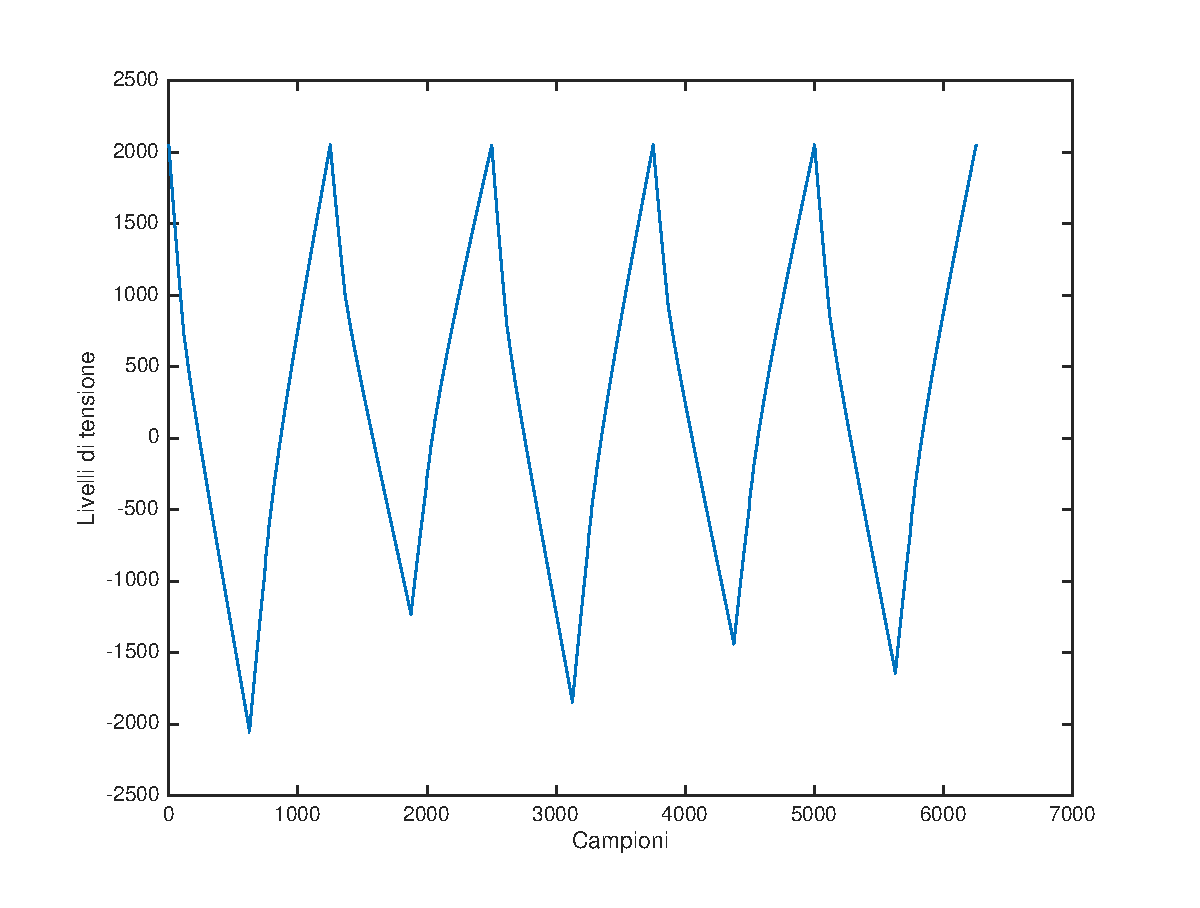
\includegraphics[scale=0.52]{cap5/cinquesegnalidis}
		\caption{Segnale di modulazione compensato, costituito da cinque forme d'onda di ampiezza diversa in ordine sparso}
		\label{cinquesegnalidis}
	\end{center}
\end{figure}

L'utilizzo di questa tecnica peggiora il tempo di acquisizione di una singola misura, in quanto, ora, un singolo valore di distanza è ottenuto dalla media dei $5$ valori ricavati utilizzando i $5$ segnali con ampiezze differenti.

Questo approccio, tuttavia, permette di scorrelare l'errore di misura provocato dallo sfasamento iniziale delle frange, permettendo una riduzione teorica di $\sqrt{5}$ sulla deviazione standard della misura. 

Tramite la prova a bersaglio fisso si è notato un miglioramento della deviazione standard di un fattore $2$, leggermente minore del risultato teorico atteso ($\sqrt{5} \approx 2.24$). La deviazione standard relativa su $1000$ misure effettuate ad una distanza di $50 cm$ dal bersaglio è passata da $4 \cdot 10^{-4}$ a $2.5 \cdot 10^{-4}$. 

\begin{figure}
\centering
\subfigure[Misure di distanza e media]
{\label{misfisso4a}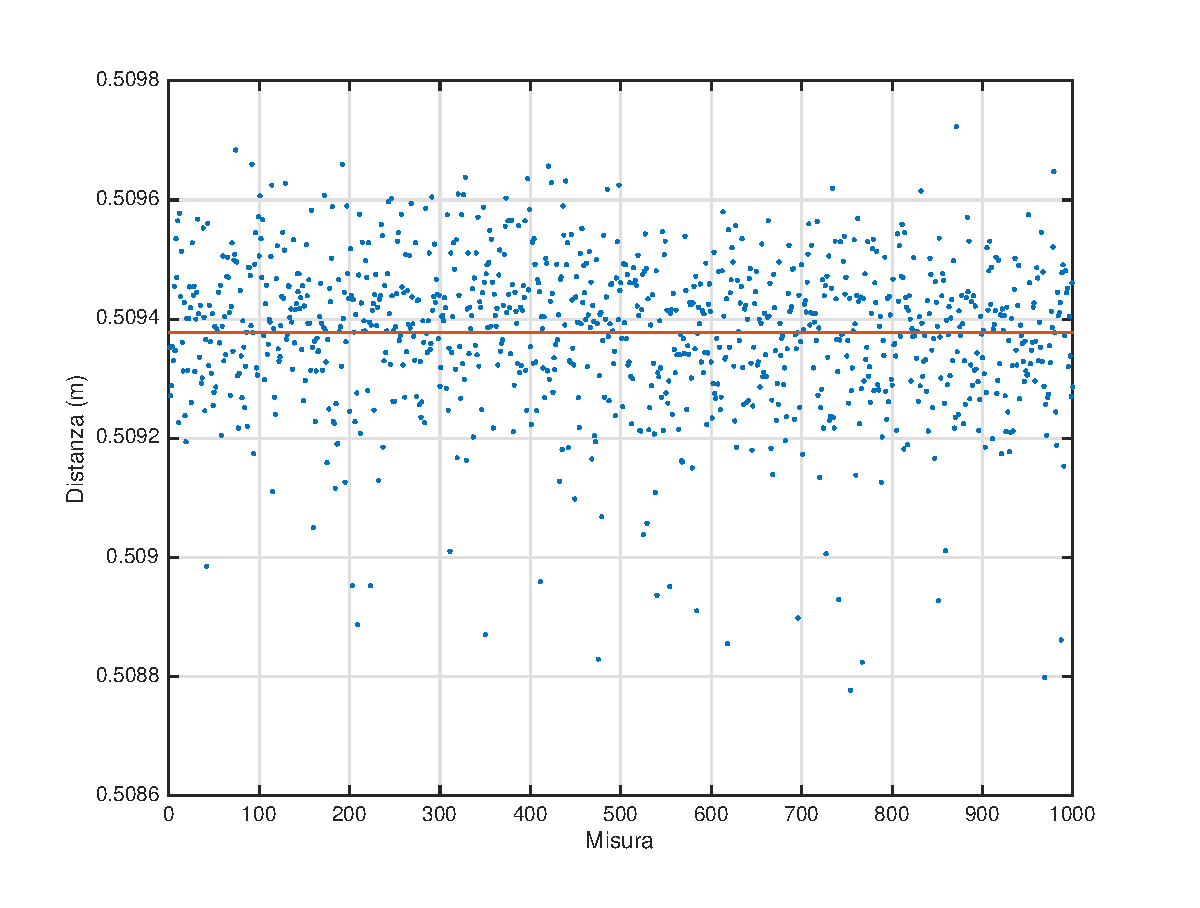
\includegraphics[scale=.5]{cap5/misfisso4a}}
\end{figure}
\begin{figure}
	\centering
\subfigure[Distribuzione dei valori misurati rispetto alla media]
{\label{misfisso4b}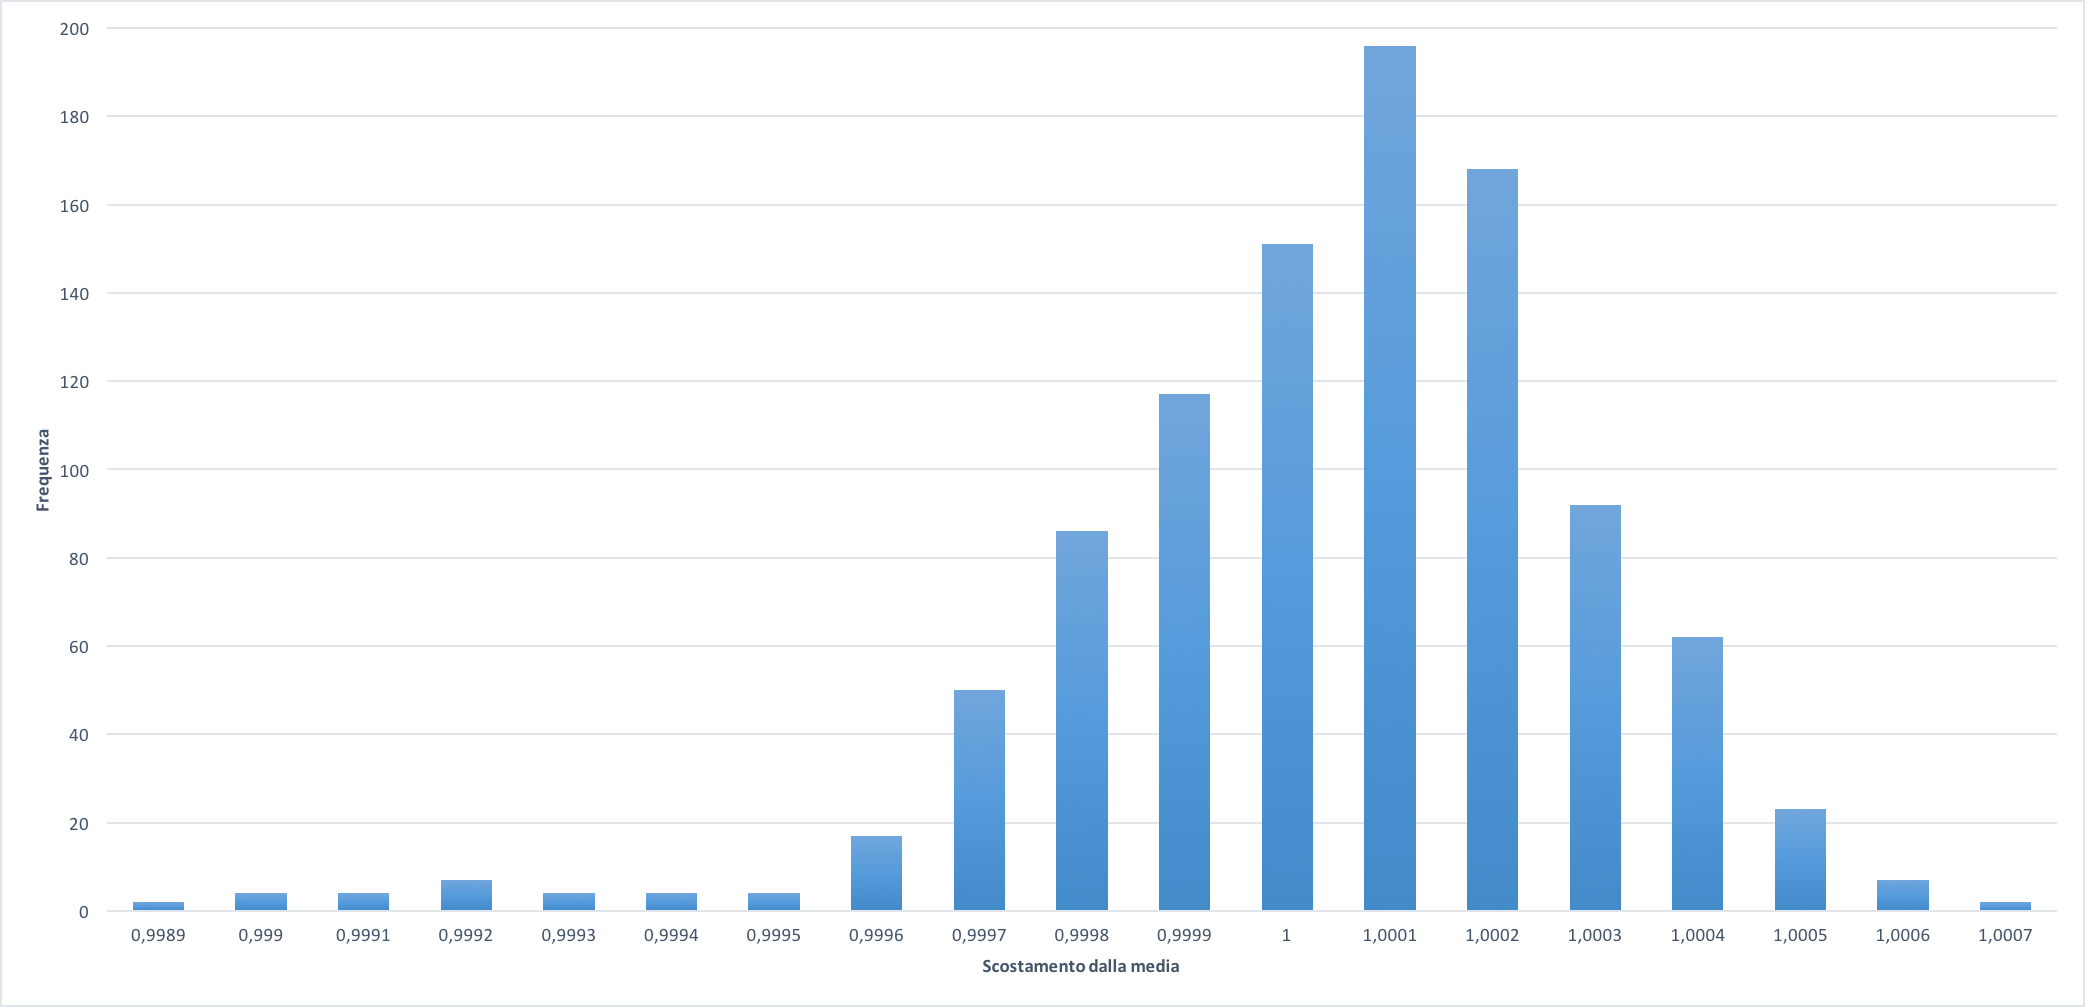
\includegraphics[scale=.3]{cap5/misfisso4b}}
\caption{Misure a bersaglio fisso con i 5 segnali di modulazione}\label{misfisso4}
\end{figure}

\begin{figure}  
  \begin{center}
    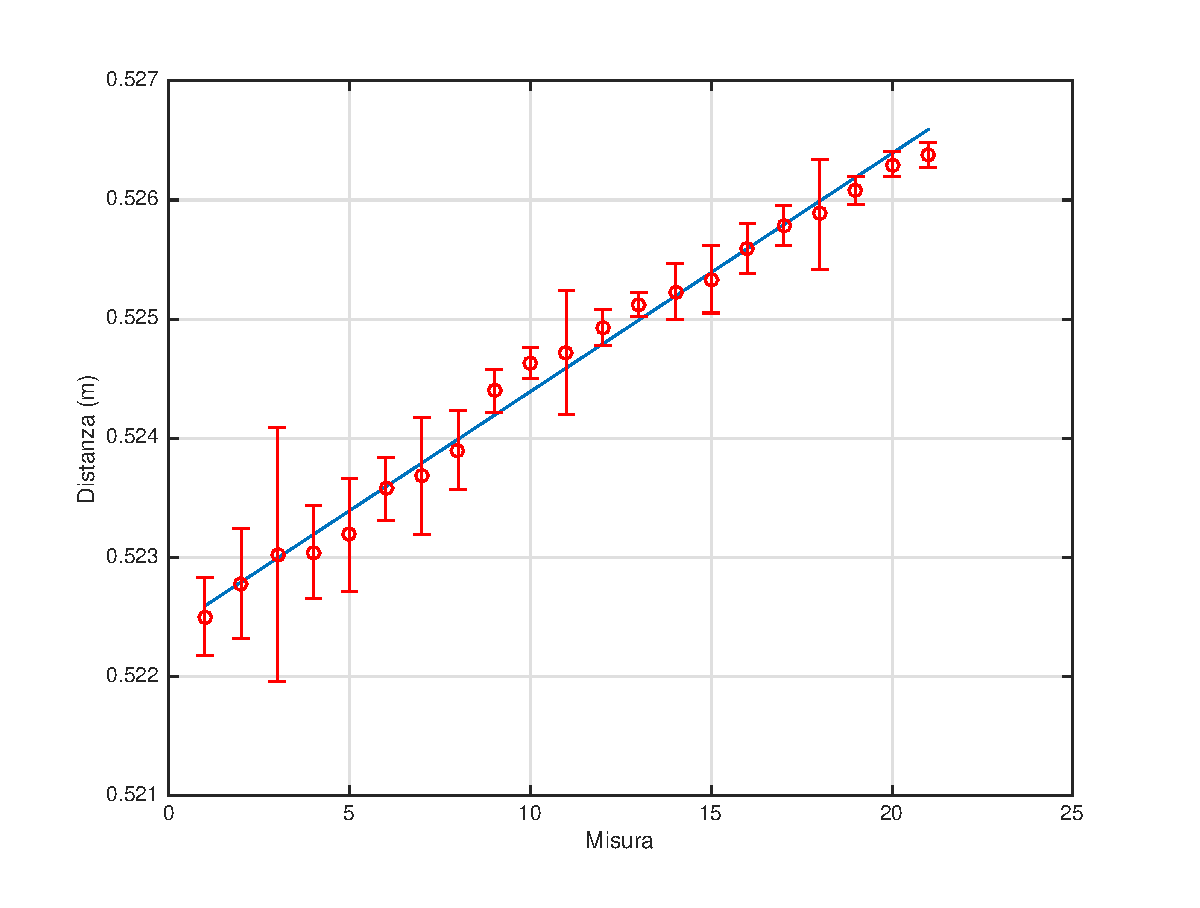
\includegraphics[scale=0.5]{cap5/mismobile4}
    \caption{Misure di distanza a bersaglio mobile effettuate su $200\mu m$ di spostamento con i 5 segnali di modulazione}
    \label{mismobile4}
  \end{center}
\end{figure}

L'introduzione di questa tecnica migliora anche la linearità dello strumento, come è chiaramente verificabile attraverso la prova a bersaglio mobile (Figura \ref{mismobile4}).

L'errore picco-picco misurato con questa prova è di $451 \mu m$, mentre l'RMS è $142 \mu m$.

Rispetto al caso precedente l'errore picco picco diminuisce di un fattore $2$, mentre l'RMS dell'errore rispetto alla retta ideale migliora di un fattore $5$.

\subsection{Sottrazione del residuo}
Come già trattato nei capitoli precedenti, l'algoritmo usato per calcolare l'FFT interpolata a 2 punti con finestra di \textit{Hanning} fa uso del bin di ampiezza massima e del bin di ampiezza maggiore scelto tra il precedente ed il successivo.

Analizzando il segnale in arrivo dal sensore laser in assenza di ostacolo, si è notata la presenza di un residuo causato dallo sottrazione non perfetta presente nello stadio analogico. Tale residuo è un errore deterministico che può influenzare negativamente la scelta del bin laterale nella algoritmo di FFT interpolata, poiché nella maggior parte dei casi essi, rispetto al massimo bin, avranno ampiezze relativamente basse e comparabili al segnale contenuto nel residuo. Questo può portare ad un errore nella stima del bin interpolato e quindi influenzare negativamente la precisione della misura.

Per cercare di mitigare l'effetto del rumore deterministico causato dal residuo si è deciso di procedere sottraendo al segnale interferometrico acquisito il suo residuo.

All'avvio dello strumento, con il sensore in assenza di ostacolo, si acquisiscono e mediano $1000$ segnali in assenza di frange. Il risultato della media è un segnale che chiamiamo "residuo". Perciò, per ogni successiva acquisizione di segnale interferometrico, si procede alla sottrazione del residuo al segnale acquisito.

La sottrazione è effettuata al momento dell'acquisizione del segnale, perciò le componenti del residuo sono sottratte sia in ampiezza che in frequenza. 

Utilizzando questa tecnica si è notato un miglioramento delle prestazioni dello strumento a basse frequenze. Ciò accade perché il residuo estratto è correlato al rumore della misura solo per determinate frequenze e la sottrazione del residuo su tutto lo spettro porta, per frequenze maggiori, all'aggiunta di ulteriore rumore alla misura.

Per mantenere i vantaggi della sottrazione del residuo a basse frequenze senza peggiorare la misura ad alte frequenze si è deciso di applicare un filtro passa-basso al residuo acquisito.

Sperimentalmente si è verificato che sottraendo il residuo per frequenze più basse di $1 \div 1.5MHz$ si ha un miglioramento della deviazione standard relativa della misura, mentre per frequenze più elevate la sottrazione del residuo porta ad un peggioramento della misura.
Per queste ragioni si è scelto in modo conservativo come frequenza di taglio del filtro passa-basso $1MHz$, per evitare di aggiungere ulteriore rumore alla misura.


\begin{table}[H]
\centering
\begin{tabular}{c|l|l|}
\multicolumn{1}{l|}{} & \multicolumn{2}{c|}{\textbf{Deviazione standard relativa}} \\ \hline
\multicolumn{1}{l|}{\textbf{\begin{tabular}[c]{@{}l@{}}Frequenza \\ (Distanza)\end{tabular}}} & \textbf{con sottrazione del residuo} & \textbf{senza sottrazione} \\ \hline
\textbf{\begin{tabular}[c]{@{}c@{}}800 KHz\\ (ca. 20cm)\end{tabular}}  & $2 \cdot 10^{-4} \div 3 \cdot 10^{-4}$ & $3 \cdot 10^{-4} \div 4 \cdot 10^{-4}$   \\
\textbf{\begin{tabular}[c]{@{}c@{}}1.5 MHz\\ (ca. 40cm)\end{tabular}} & $4 \cdot 10^{-4} \div 5 \cdot 10^{-4}$  & $4 \cdot 10^{-4} \div 5 \cdot 10^{-4}$ \\
\textbf{\begin{tabular}[c]{@{}c@{}}3.5 MHz\\ (ca. 90cm)\end{tabular}} & $6 \cdot 10^{-4} \div 7 \cdot 10^{-4}$ & $5 \cdot 10^{-4} \div 6 \cdot 10^{-4}$
\end{tabular}
\caption{Valori sperimentali di deviazione standard relativa calcolati su $1000$ misure a ostacolo fisso}
\label{tab:residuofatt}
\end{table}
In Tabella \ref{tab:residuofatt} è mostrato il range di deviazioni standard relative misurate al variare della frequenza.
Anche per queste implementazioni sono state eseguite le consuete prove descritte nei paragrafi precedenti.

\begin{figure}[H] 
  \begin{center}
    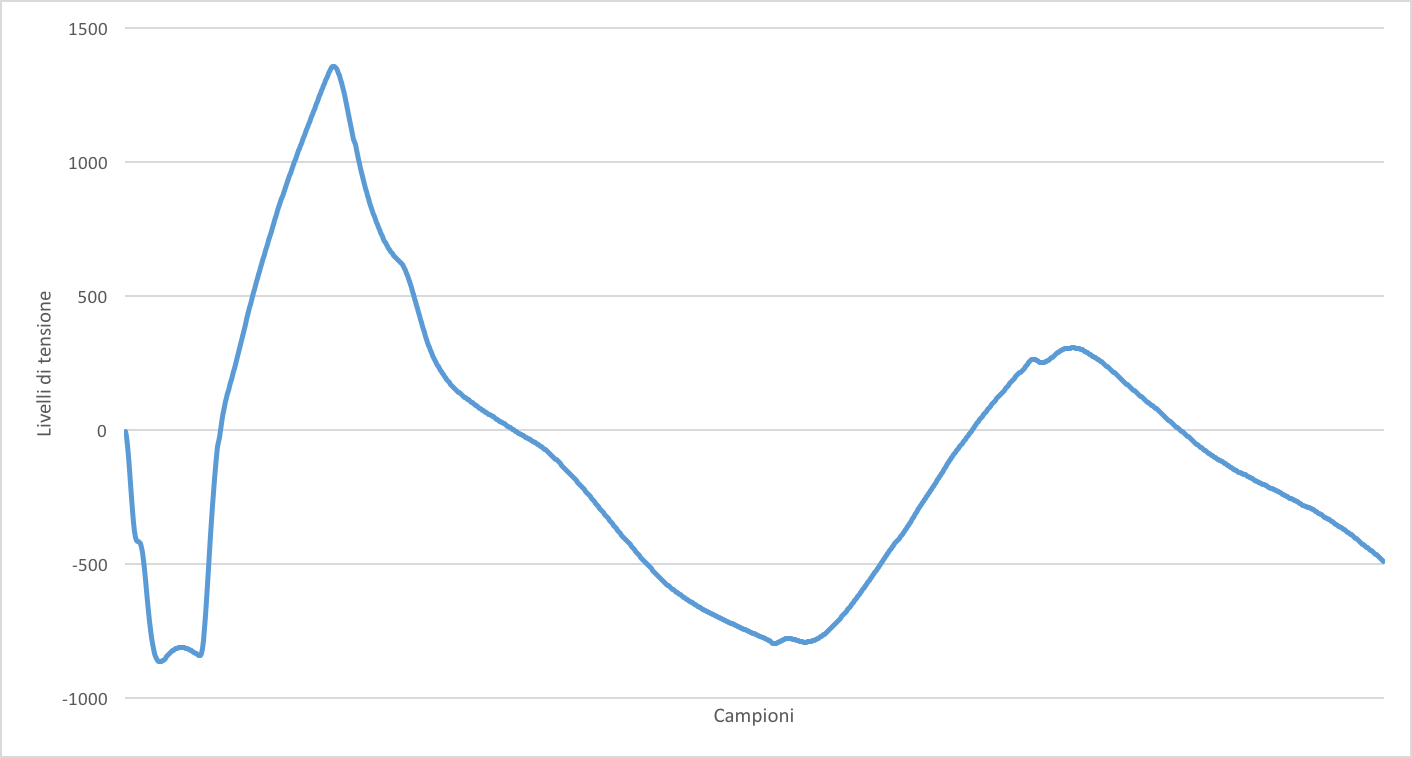
\includegraphics[scale=0.5]{cap5/residuo}
    \caption{Residuo filtrato passa-basso con frequenza di taglio a 1 MHz}
    \label{residuo}
  \end{center}
\end{figure}

Nella prova a bersaglio fisso (Figura \ref{misfisso5}) si è notato un miglioramento non sostanziale rispetto al caso senza sottrazione del residuo. Questo accade a causa del posizionamento del bersaglio; infatti, alla distanza di $50 cm$, la frequenza misurata (ca. $1.9MHz$) è al di sopra della frequenza di taglio del filtro passa-basso che agisce sul residuo estratto, rendendo la sottrazione del residuo poco efficace.

In questo caso il valore di deviazione standard relativa calcolato su $1000$ campioni vale $2.4 \cdot 10^{-4}$.

Nella Figura \ref{misfisso5b} è stata sovrapposta la distribuzione gaussiana teorica dei valori, e si può notare che i dati empirici sono aderenti ad essa.

Dai risultati ottenuti nella prova a bersaglio mobile (Figura \ref{mismobile5}) si ottiene, al contrario dell'esperimento a bersaglio fisso, un notevole miglioramento nell'accuratezza. Vi è un dimezzamento, rispetto al caso senza sottrazione del residuo, della distanza picco-picco dell'errore. Essa scende a $280 \mu m$ con un RMS pari a $124 \mu m$.
\begin{figure}[H]
	\centering
	\subfigure[Misure di distanza e media]
	{\label{misfisso5a}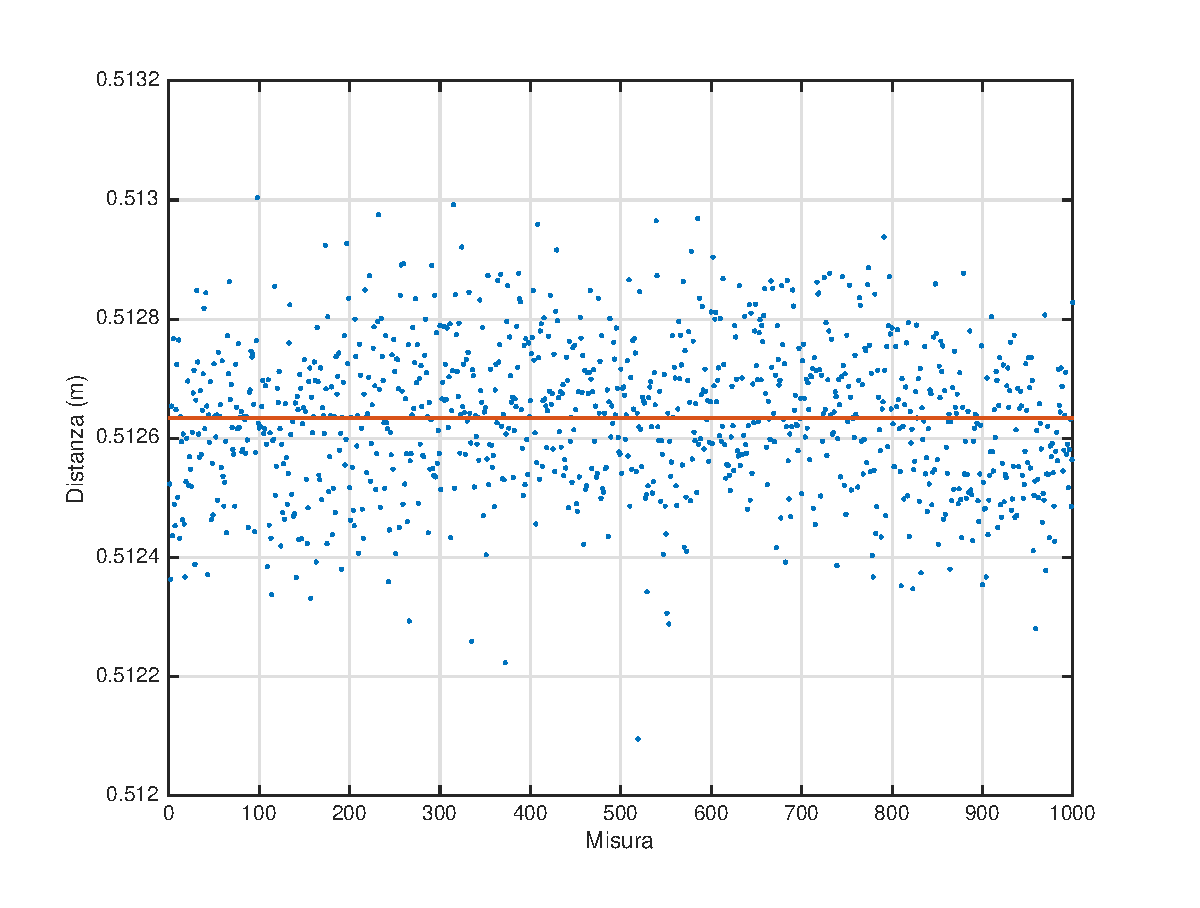
\includegraphics[scale=.5]{cap5/misfisso5a}}
\end{figure}
\begin{figure}[H]
	\centering
	\subfigure[Distribuzione dei valori misurati rispetto alla media]
	{\label{misfisso5b}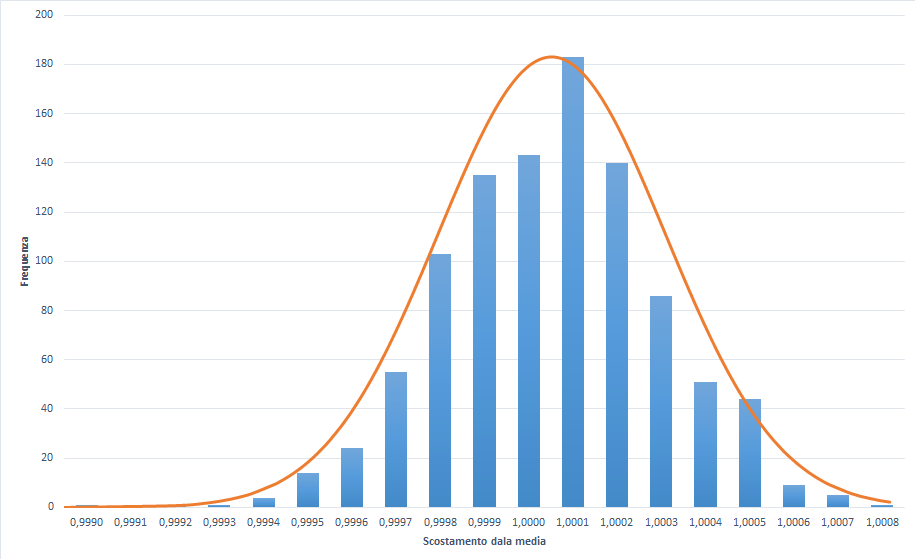
\includegraphics[scale=.4]{cap5/misfisso5b}}
	\caption{Misure di distanza a bersaglio fisso con sottrazione del residuo}\label{misfisso5}
\end{figure}
\begin{figure}[H] 
	\begin{center}
		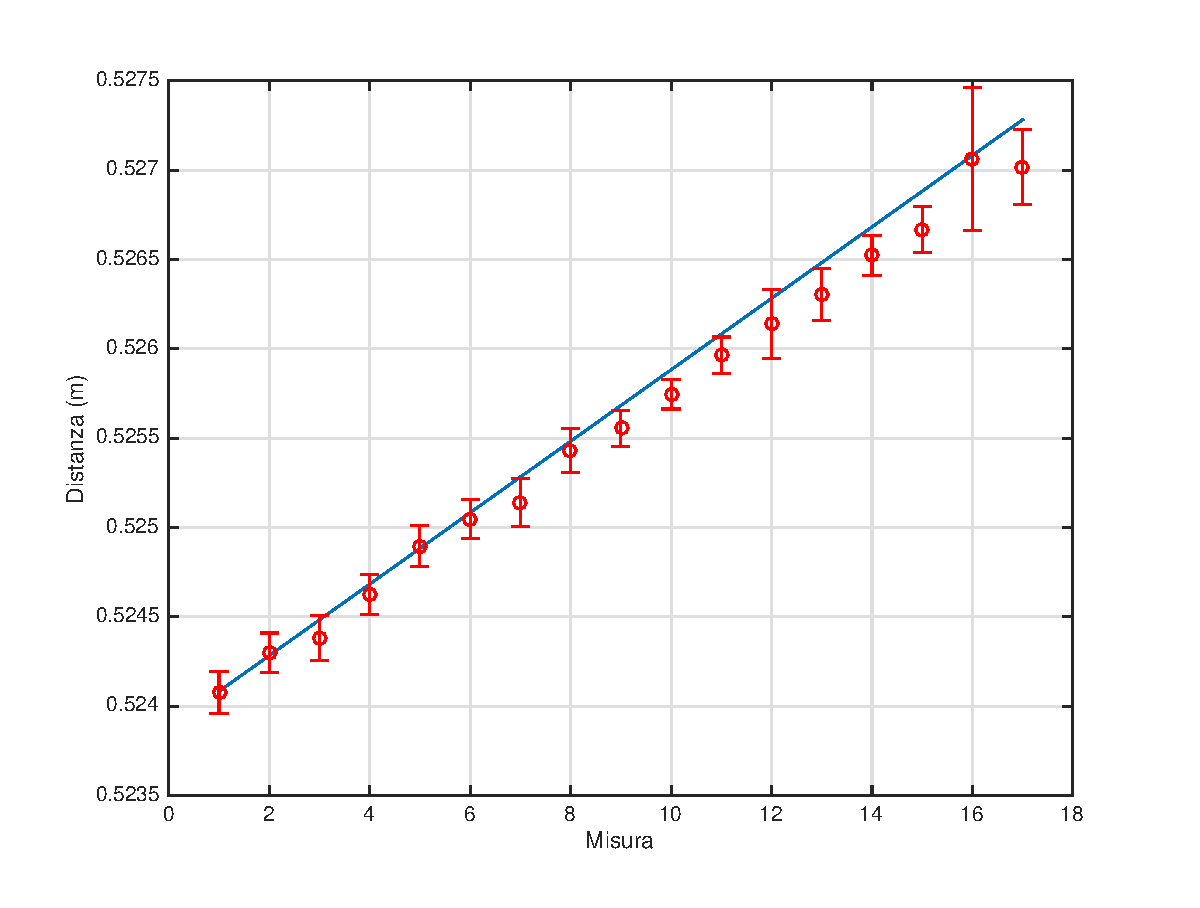
\includegraphics[scale=0.5]{cap5/mismobile5}
		\caption{Misure di distanza a bersaglio mobile con sottrazione del residuo effettuate su $200 \mu m$ di spostamento}
		\label{mismobile5}
	\end{center}
\end{figure}

\section{Prove dello strumento finale}
Alla luce dei risultati riportati nei paragrafi precedenti, nell'implementazione finale dello strumento si è deciso di utilizzare l'algoritmo a $5$ segnali di modulazione con sottrazione del residuo.

Questa scelta è stata fatta poiché l'intervallo di misura garantito permette di avere precisioni migliori a basse distanze, senza avere peggioramenti significativi nella restante zona di funzionamento del sensore.

Come anticipato in precedenza con la configurazione finale sono state eseguite due ulteriori prove a bersaglio fisso e mobile alle distanze di $20cm$ e $90cm$, i cui risultati sono riportati di seguito.

\subsection{Bersaglio fisso}
Nella prova a bersaglio fisso a $20cm$ (Figura \ref{misfisso520}) si ottiene una deviazione standard relativa di $1.32 \cdot 10^{-4}$, mentre con il bersaglio a $90cm$  (Figura \ref{misfisso590}) la deviazione standard relativa ottenuta è di $6.5 \cdot 10^{-4}$.
I risultati sono in linea con le aspettative. Le prestazioni degradano alla distanza di $90cm$ in quanto si arriva nei pressi dei limiti di funzionamento dello strumento.

\begin{figure}[H]
	\centering
	\subfigure[Misure di distanza e media]
	{\label{misfisso5a20}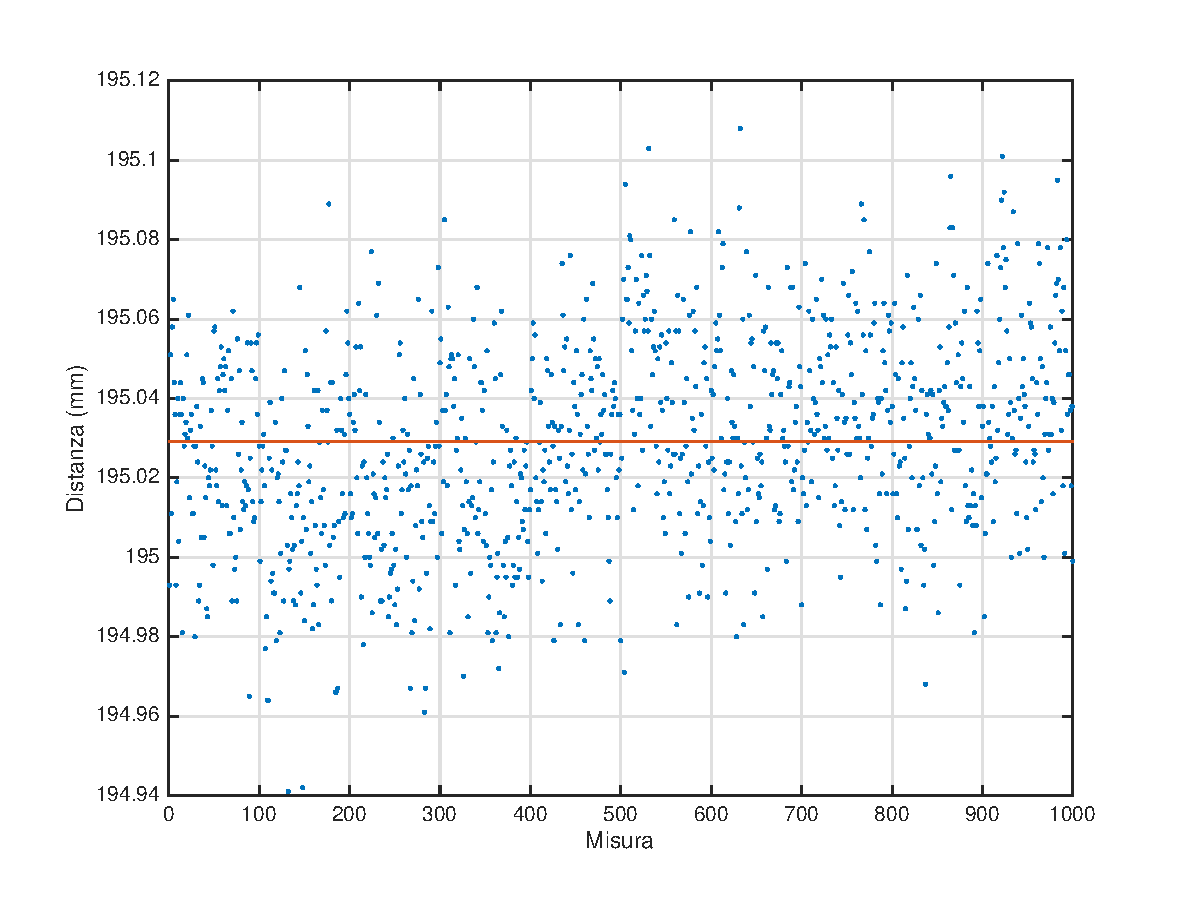
\includegraphics[scale=.5]{cap5/misfisso5a20}}
\end{figure}
\begin{figure}[H]
	\centering
	\subfigure[Distribuzione dei valori misurati rispetto alla media]
	{\label{misfisso5b20}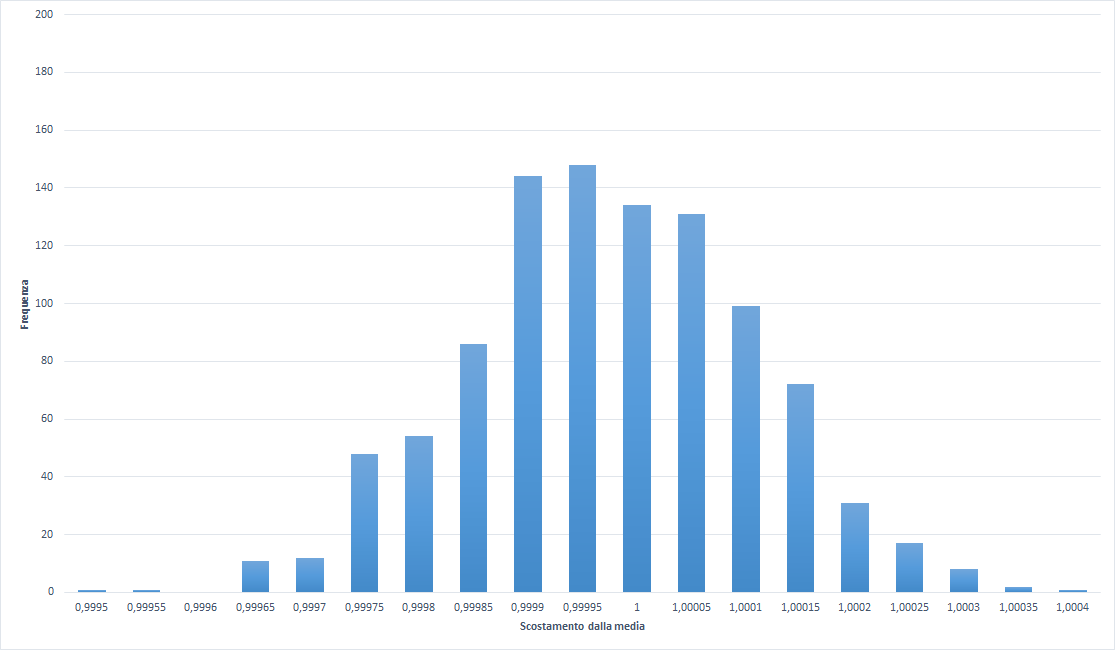
\includegraphics[scale=.35]{cap5/misfisso5b20}}
	\caption{Misure di distanza a 20cm con bersaglio fisso }\label{misfisso520}
\end{figure}
\begin{figure}[H]
	\centering
	\subfigure[Misure di distanza e media]
	{\label{misfisso5a90}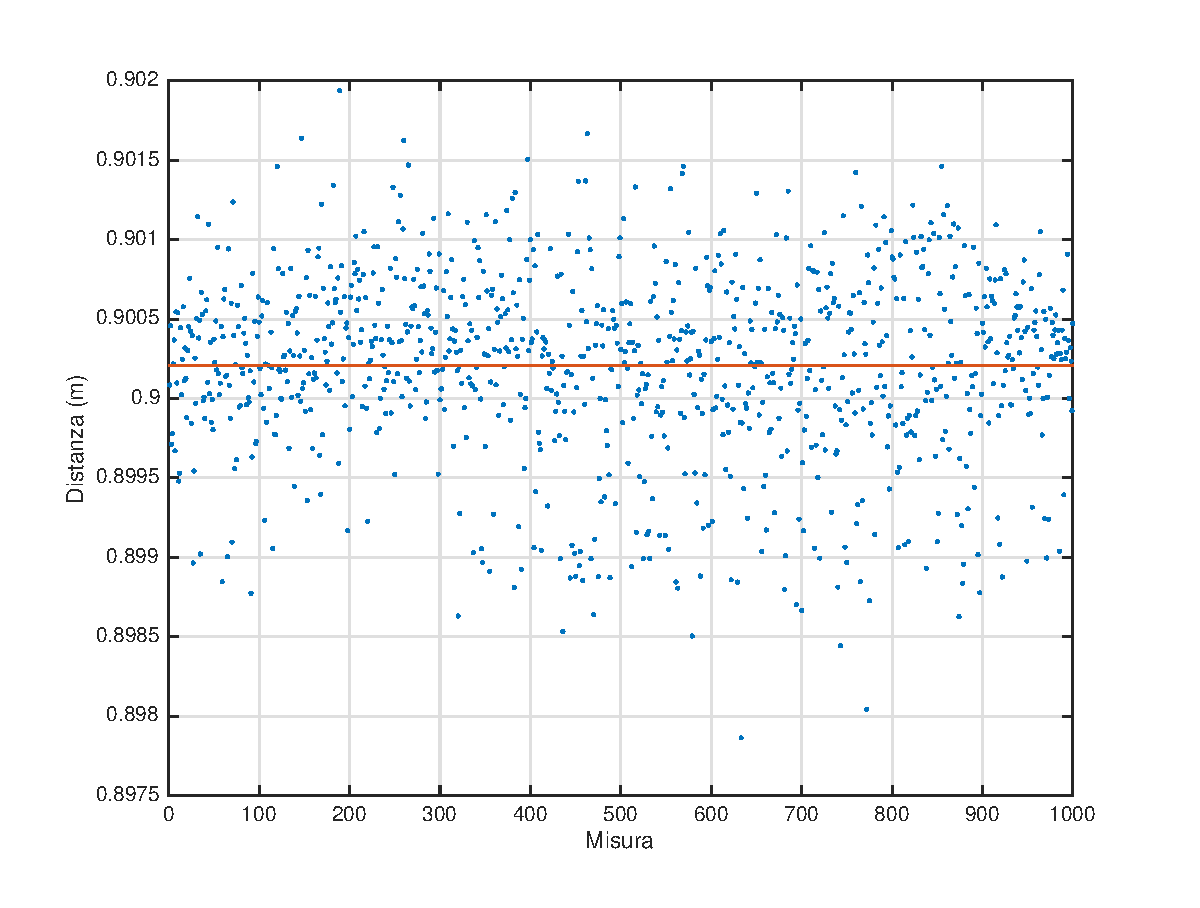
\includegraphics[scale=.5]{cap5/misfisso5a90}}
\end{figure}
\begin{figure}[H]
	\centering
	\subfigure[Distribuzione dei valori misurati rispetto alla media]
	{\label{misfisso5b90}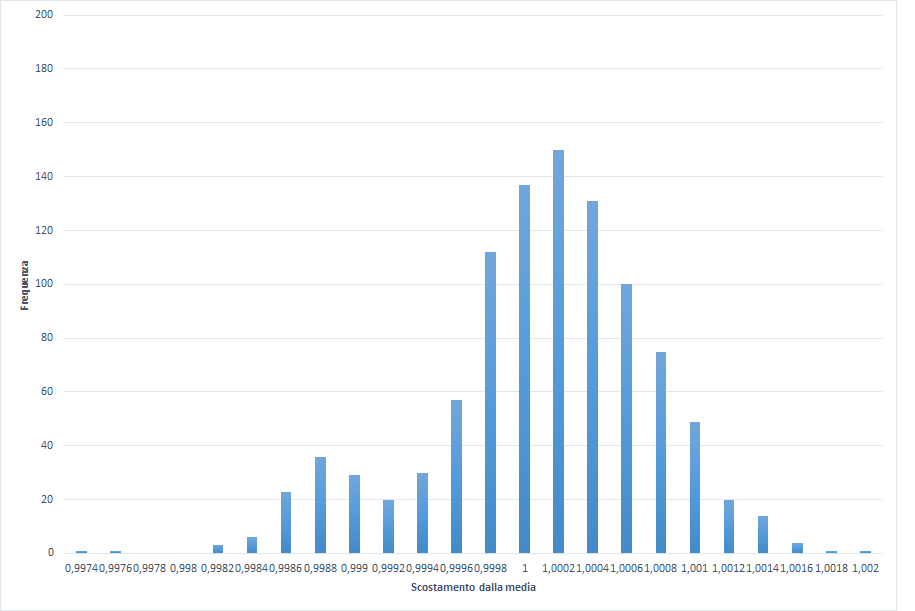
\includegraphics[scale=.4]{cap5/misfisso5b90}}
	\caption{Misure di distanza a 90cm con bersaglio fisso }\label{misfisso590}
\end{figure}

\subsection{Bersaglio mobile}

Nella prova a bersaglio mobile, anche in questo caso, i risultati sono in linea con le aspettative. 
Alla distanza di $20cm$ (Figura \ref{mismobile520}) l'errore picco-picco ottenuto vale $258 \mu m$, con un RMS di $121 \mu m$.
Alla distanza di $90cm$ (Figura \ref{mismobile590}) l'errore picco-picco ottenuto vale $ 545 \mu m$, con un RMS di $ 190 \mu m$.
In questo caso lo strumento dimostra una maggiore linearità all'aumentare della distanza, in quanto l'errore relativo a $90cm$ è minore rispetto a quello registrato a $20cm$, nonostante in valore assoluto sia maggiore.
\begin{figure}[H]  
	\begin{center}
		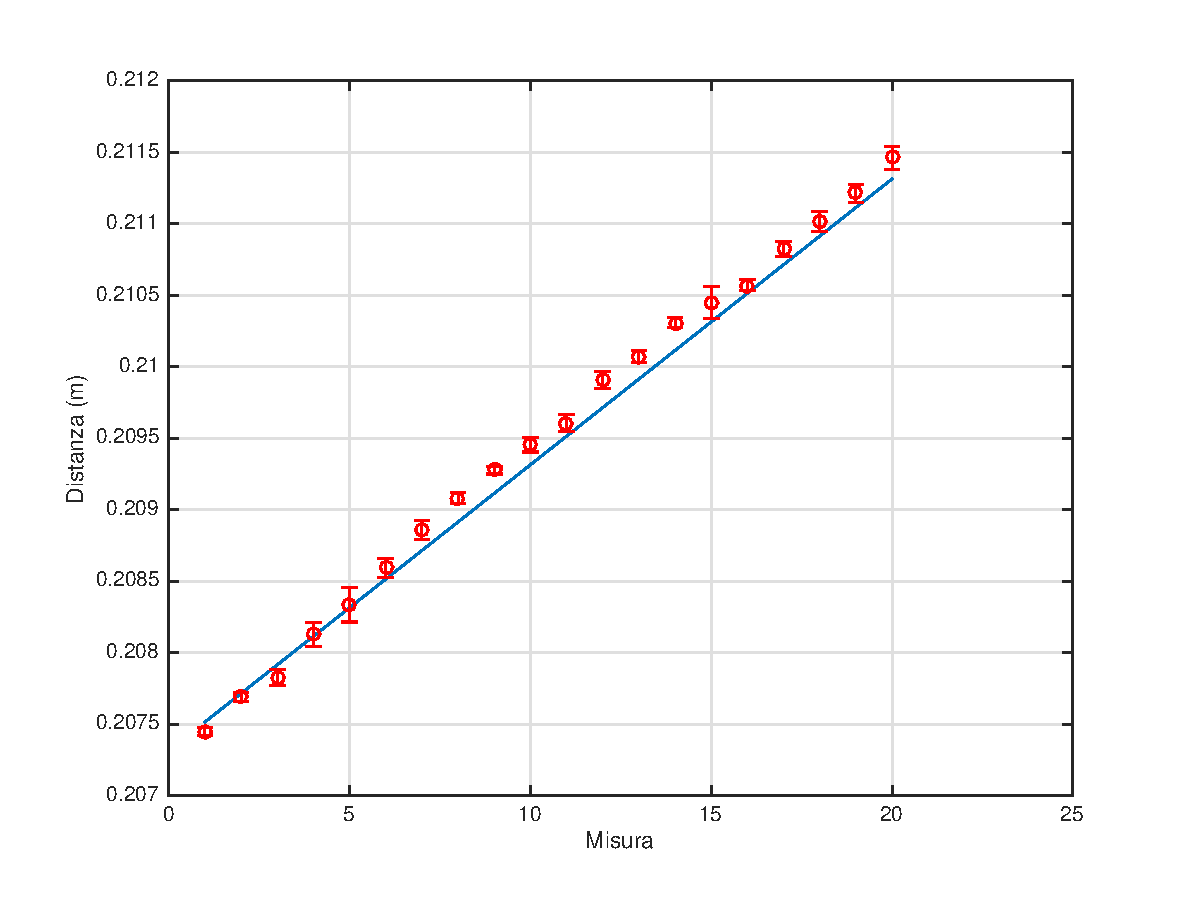
\includegraphics[scale=0.5]{cap5/mismobile520}
		\caption{Misure di distanza a $20cm$ con bersaglio mobile effettuate su $200 \mu m$ di spostamento}
		\label{mismobile520}
	\end{center}
\end{figure}
\begin{figure}[H] 
	\begin{center}
		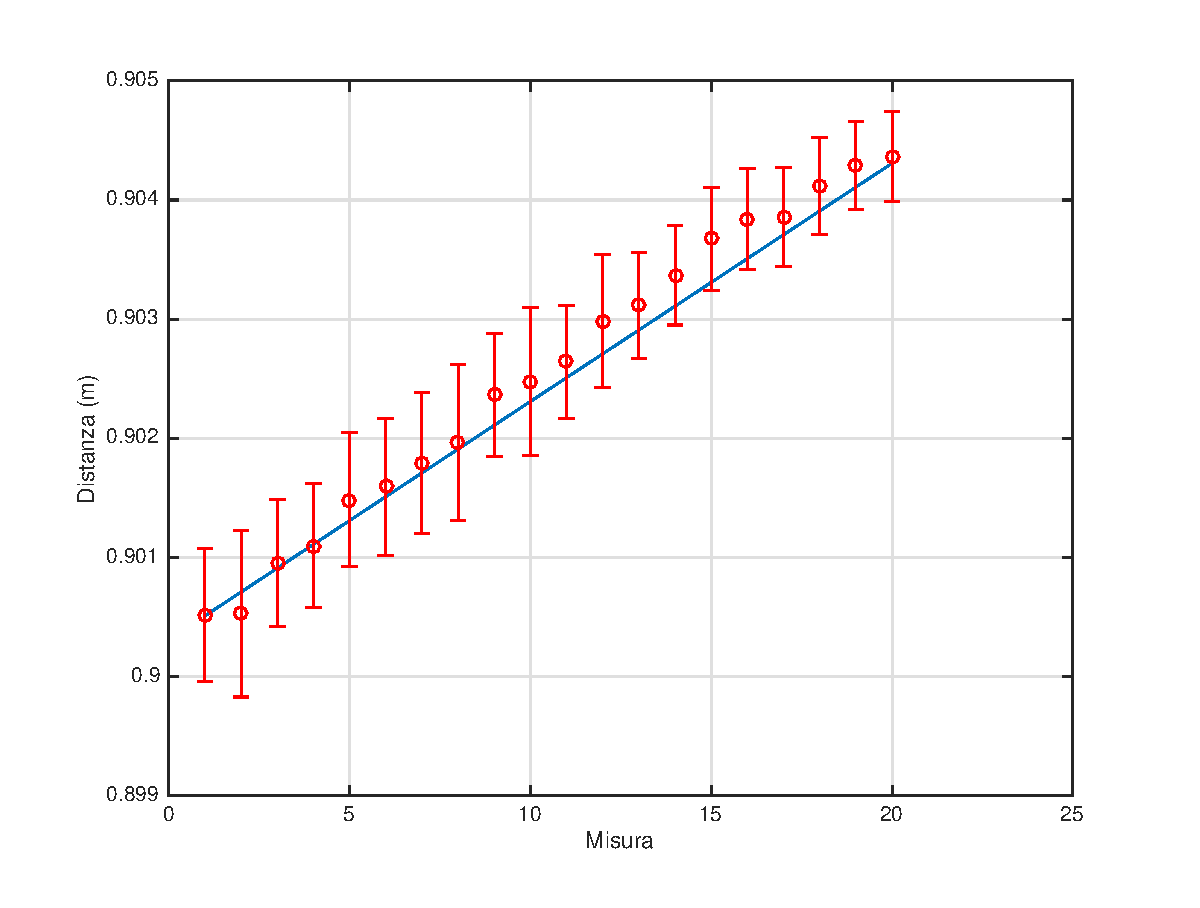
\includegraphics[scale=0.5]{cap5/mismobile590}
		\caption{Misure di distanza a $90cm$ con bersaglio mobile effettuate su $200 \mu m$ di spostamento}
		\label{mismobile590}
	\end{center}
\end{figure}

\subsection{Range di misura}
Con lo strumento nella sua configurazione finale è stata anche misurata la deviazione standard relativa su $100$ misure a differenti distanze al fine di determinare il range di distanza misurabile dallo strumento. 


I risultati ottenuti sono riportati nel grafico seguente ed è possibile notare che la misura si mantiene in valori di deviazione standard relativa accettabili in un range che varia da $15cm$ a $110cm$. 

Oltre questo range la deviazione standard relativa della misura supera valori di $10^{-3}$, rendendo scarsa la precisione della misura.

Osservando l'andamento dell'ampiezza dei bin massimi in funzione della distanza (Figura \ref{ampbin}) è facilmente intuibile la motivazione della massima distanza misurabile. Per valori di distanza che superano i $110cm$ l'ampiezza del bin è troppo bassa per poter essere distinta dal rumore elettronico che lo strumento presenta, rendendo così la misura inaffidabile.

La minima distanza misurabile, invece, dipende dal numero di bin iniziali che si decide di scartare. Si è verificato che i bin precedenti al quarto sono influenzati dalle componenti in bassa frequenza presenti nel segnale interferometrico, e quindi non possono portare informazioni utili alla misura.

Nell'implementazione finale dello strumento i bin precedenti al quarto non vengono considerati.
\begin{figure}[H]
	\begin{center}
		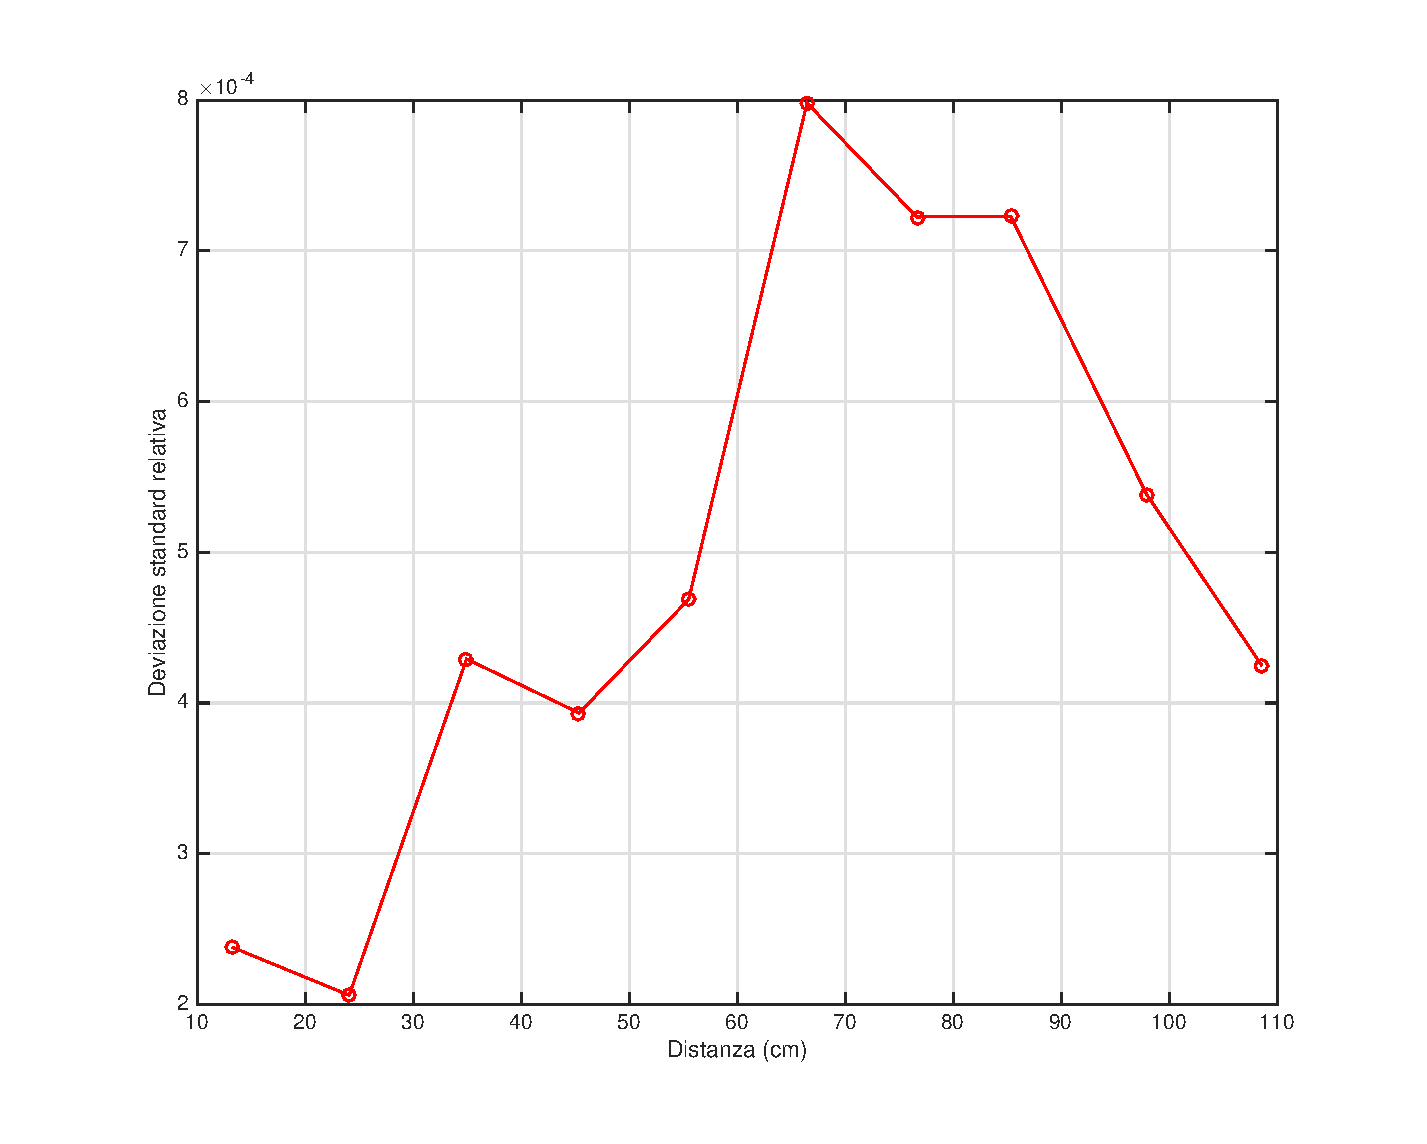
\includegraphics[scale=0.45]{cap5/rangemis}
		\caption{Andamento della deviazione standard relativa in funzione della distanza}
		\label{rangemis}
	\end{center}
\end{figure}
\begin{figure}[H]
	\centering
	\subfigure[Sempiperiodo di discesa]
	{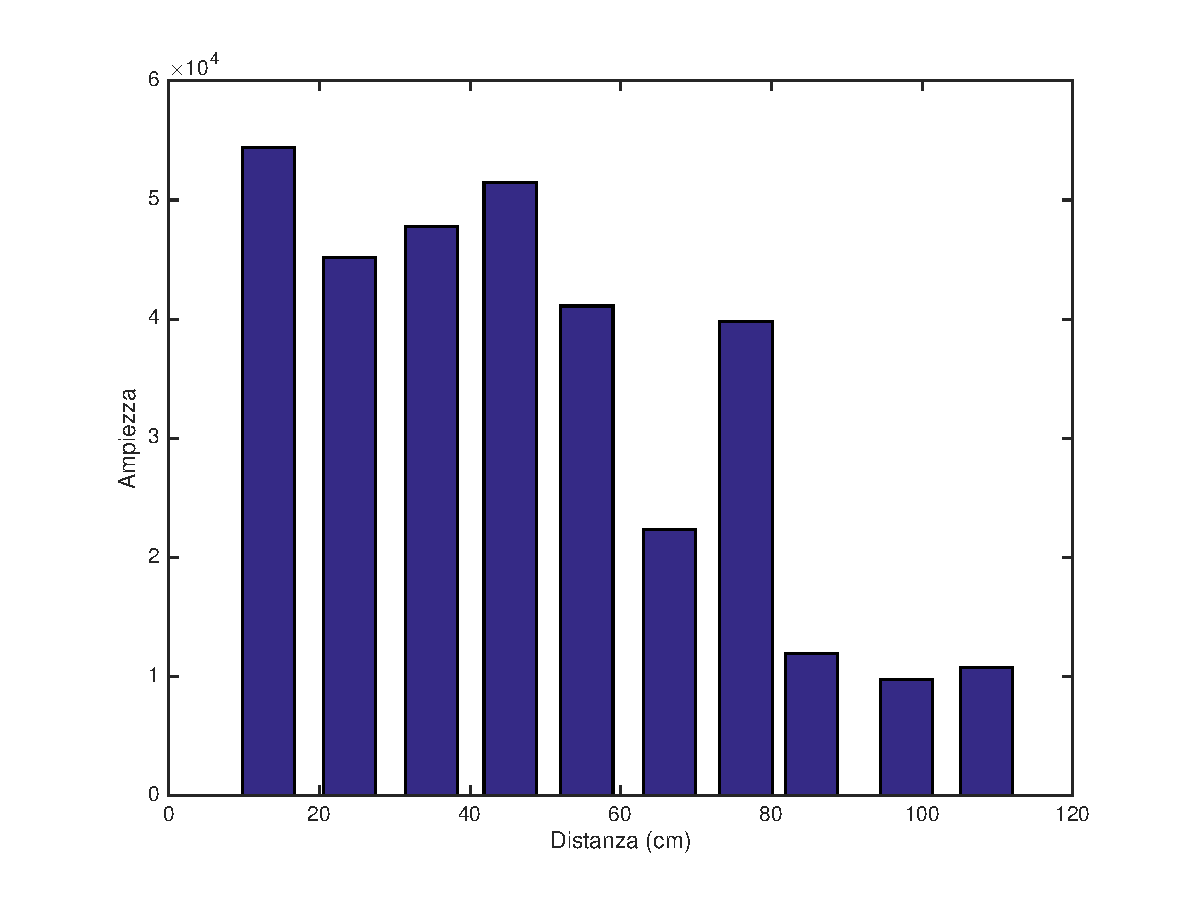
\includegraphics[scale=.6]{cap5/ampbindiscesa}}
\end{figure}
\begin{figure}[H]
	\centering
	\subfigure[Semiperiodo di salita]
	{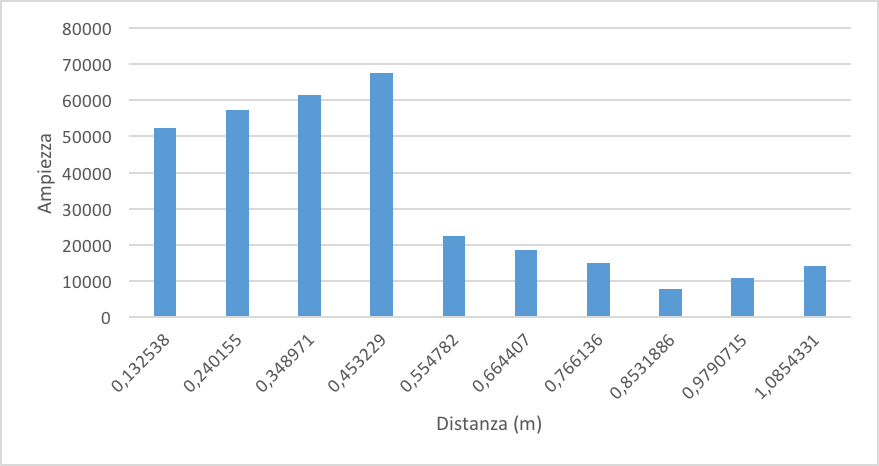
\includegraphics[scale=.6]{cap5/ampbinsalita}}
	\caption{Ampiezza del massimo bin in funzione della distanza}\label{ampbin}
\end{figure}

\subsection{Prestazioni}
Qui di seguito si riassumono le prestazioni di misura dello strumento finale:
\begin{itemize}
	\item Range spaziale di misura: $10cm \div 110cm$
	\item Minima incertezza relativa della misura di distanza: $8 \cdot 10^{-4}$
	\item Massima incertezza relativa della misura di distanza: $2 \cdot 10^{-4}$
	\item Frequenza massima teorica di misura: $1$ misura valida ogni $208 \mu s$ ($4.8 KHz$).
	
	A causa di mancanza di area nell'FPGA in uso non è stato possibile raggiungere le prestazioni di misura teoriche. Con un'acquisizione continua della misura si è riusciti ad ottenere una misura di distanza valida ogni $20 ms$ ($50 Hz$). L'occupazione in termini di area dell'algoritmo dell'FFT non ha permesso di implementare in hardware l'intero algoritmo di FFT interpolata e calcolo della distanza, rendendo così necessario l'uso di un microcontrollore per la conclusione dell'elaborazione numerica dei risultati dell'FFT.
	
	La logica di scambio dati FPGA-microcontrollore e l'overhead causato dalla connessione \textit{Ethernet} tra scheda e PC sono le cause più probabili del degrado della prestazione in termini di velocità di acquisizione di una singola misura.
\end{itemize}

\section{Cenni su un'ulteriore ottimizzazione nell'algoritmo di compensazione}
Osservando la forma d'onda finale di modulazione ricavata nei passi precedenti (Figura \ref{ondafinale}) è facile notare come la curva non sia perfettamente liscia e presenti delle irregolarità in alcune zone (Figura \ref{irrzoom}).
Queste irregolarità derivano da imperfezioni introdotte durante il calcolo della curva della variazione delle frequenze di frangia (passo $3$ dell'algoritmo presentato nel paragrafo \ref{subsec:metodocomp}) che viene interpolata linearmente punto per punto provocando così un andamento non liscio.
\begin{figure}  
	\begin{center}
		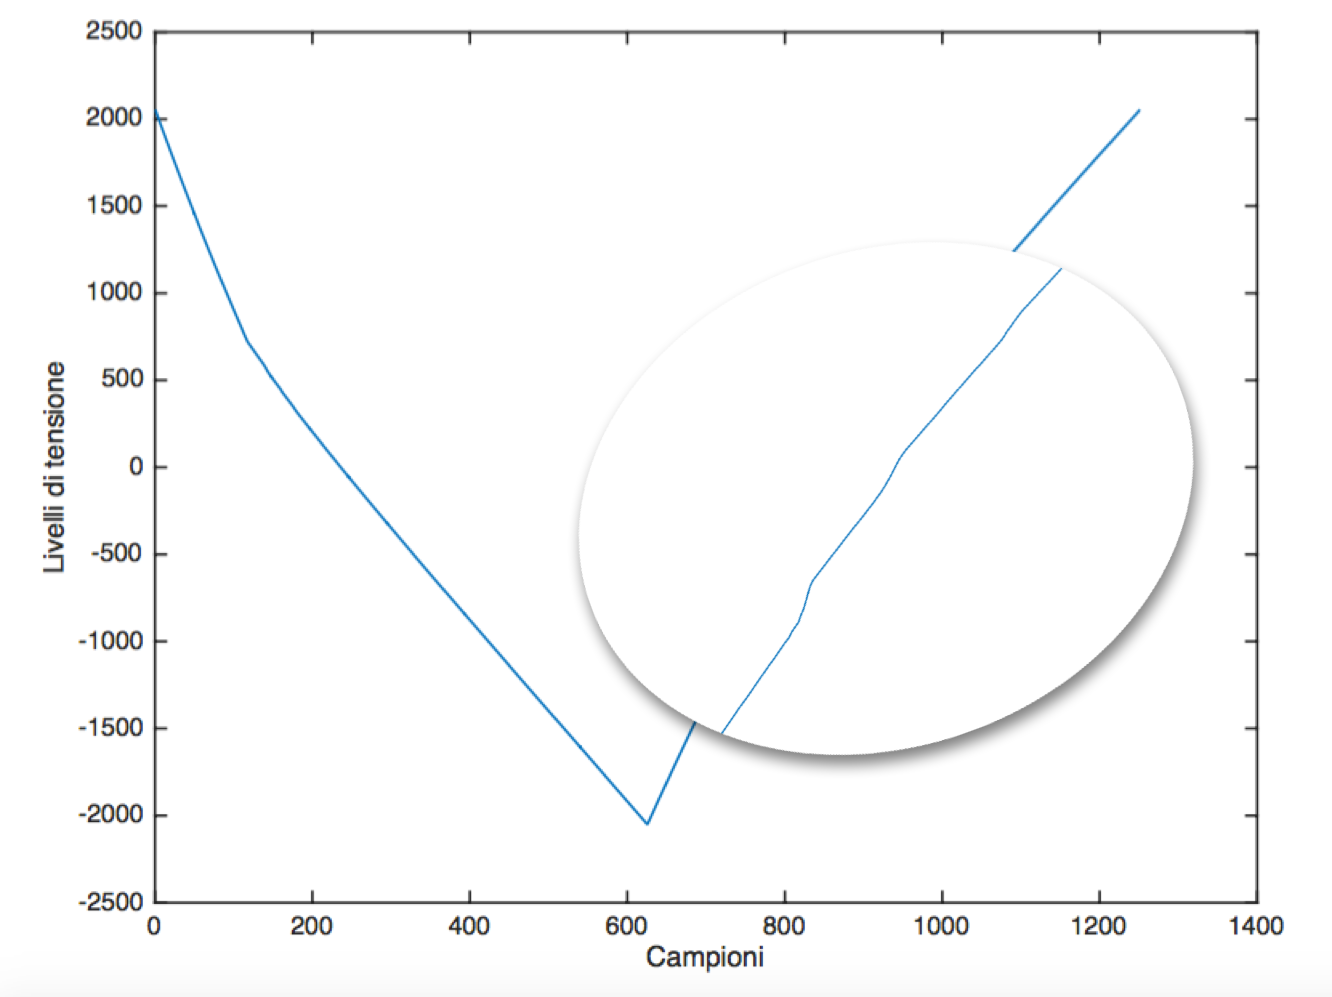
\includegraphics[scale=0.2]{cap5/irrzoom}
		\caption{Irregolarità nel segnale di modulazione}
		\label{irrzoom}
	\end{center}
\end{figure}

Queste irregolarità possono influire negativamente durante la modulazione del laser e quindi peggiorare la precisione e l'accuratezza della misura. Per questo motivo è stato deciso di approssimare la curva delle frequenze di frangia utilizzando un processo di \textit{curve fitting} polinomiale di $3\degree$ grado invece che un'interpolazione lineare punto-punto. In Figura \ref{curvefittingfreq} è mostrata in blu la curva delle frequenze di frangia estratta in un semiperiodo di modulazione e in rosso la sua approssimazione polinomiale di $3\degree$ grado.
\begin{figure}[H]  
	\begin{center}
		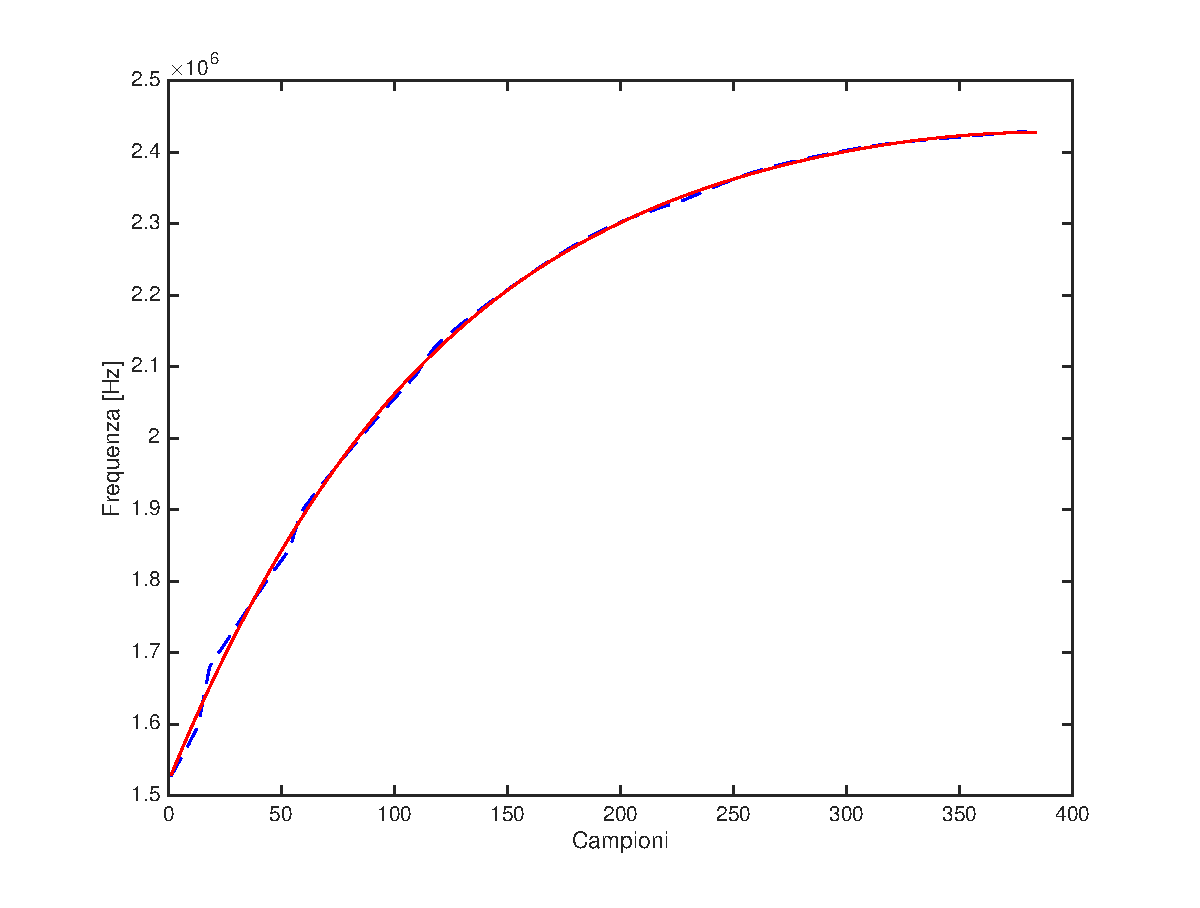
\includegraphics[scale=0.5]{cap5/curvefittingfreq}
		\caption{Curva mediata delle frequenze in un semiperiodo di modulazione con curve fitting polinomiale di $3\degree$ grado}
		\label{curvefittingfreq}
	\end{center}
\end{figure}

Un ulteriore ottimizzazione effettuata sull'algoritmo di compensazione del segnale di modulazione riguarda il calcolo iterativo del fattore moltiplicativo (passo 4 dell'algoritmo presentato nel paragrafo \ref{subsec:metodocomp}). Per valutare la bontà del fattore moltiplicativo calcolato si è scelto di utilizzare la massima variazione relativa della frequenza di frangia rispetto alla media invece che la deviazione standard relativa, questo per permettere un miglior appiattimento della curva delle frequenze.

La curve ricavate dal calcolo iterativo del fattore moltiplicativo sono presentate in Figura \ref{mulfactnew}. Si può notare che, anche in questa versione ottimizzata dell'algoritmo di compensazione, il minimo della curva si trova nell'intorno di $0.2$, sia per il fronte di salita che per il fronte di discesa. I valori esatti ricavati sono $0.16$ per il fronte di discesa e $0.27$ per il fronte di salita. Essi variano leggermente rispetto a quelli ricavati con l'algoritmo non ottimizzato. 
Come da previsione, la forma d'onda finale (Figura \ref{newondafinale}), ricavata con l'utilizzo dell'algoritmo ottimizzato, possiede un andamento più liscio rispetto alla forma d'onda impiegata fino ad adesso.

\begin{figure}[H]
	\centering
	\subfigure[Semiperiodo di discesa]
	{\label{}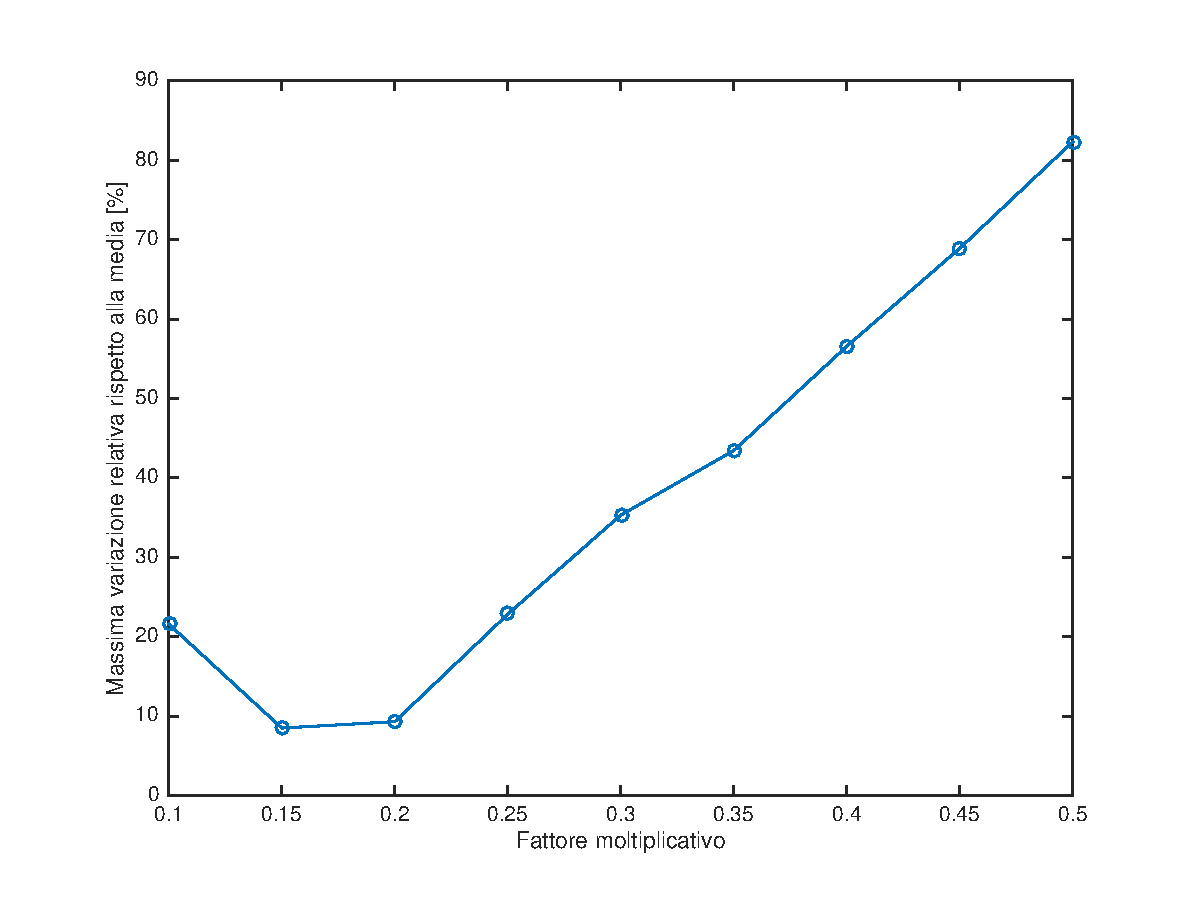
\includegraphics[scale=.5]{cap5/mulfactdiscesanew}}
\end{figure}
\begin{figure}[H]
	\centering
	\subfigure[Semiperiodo di salita]
	{\label{}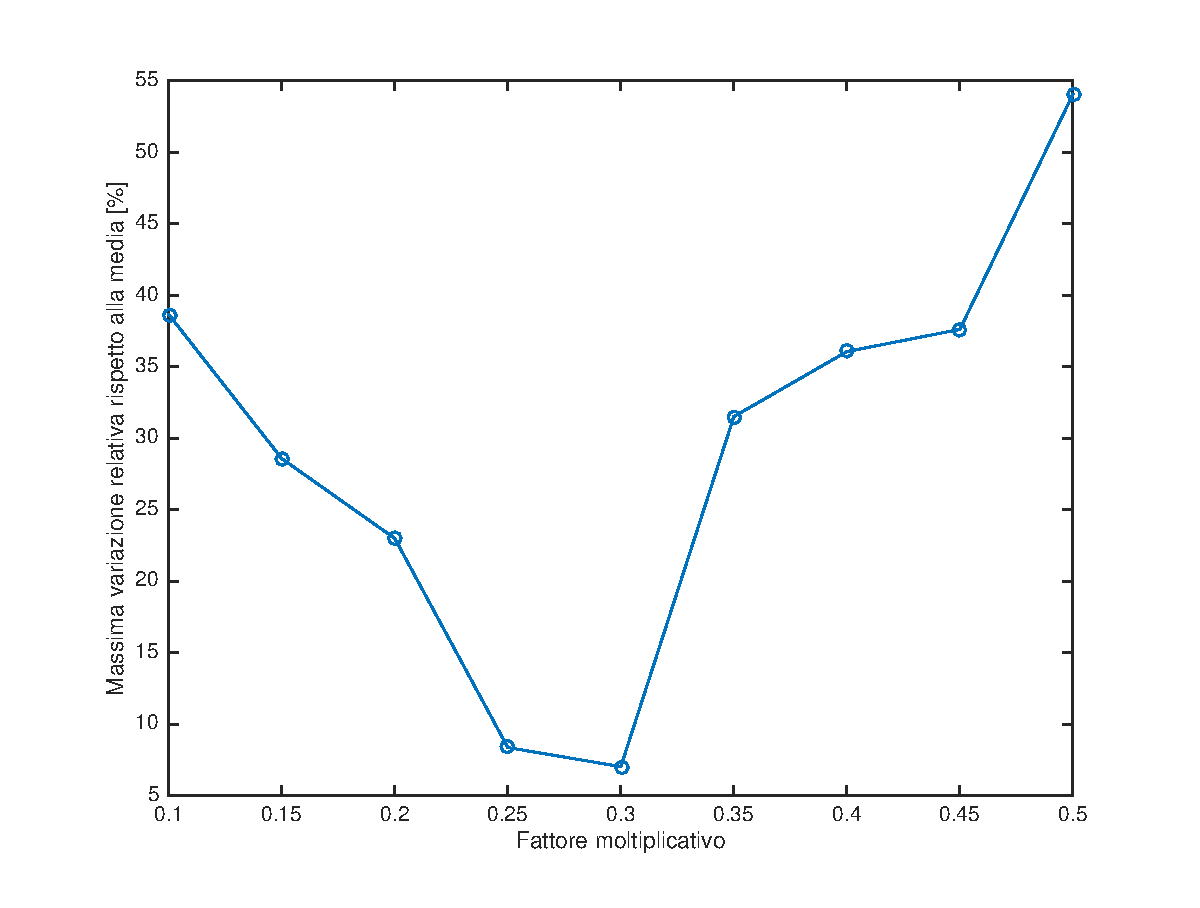
\includegraphics[scale=.5]{cap5/mulfactsalitanew}}
	\caption{Curva delle massime variazioni relative rispetto alla media dei due fronti al variare del fattore moltiplicativo}\label{mulfactnew}
\end{figure}
    \begin{figure}[H]
    	\begin{center}
    		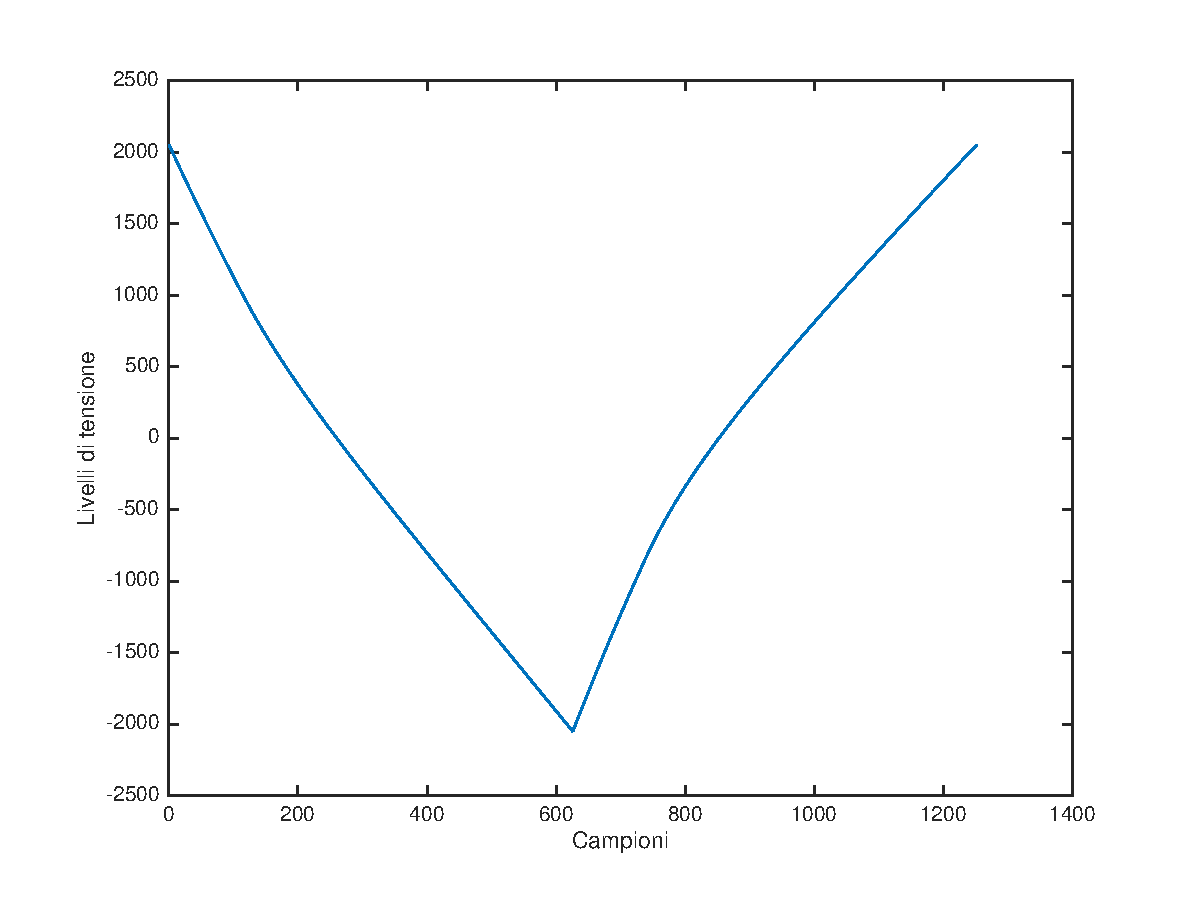
\includegraphics[scale=0.6]{cap5/newondafinale}
    		\caption{Forma d'onda finale usata per la modulazione}
    		\label{newondafinale}
    	\end{center}
    \end{figure}

\begin{figure}[H]
	\centering
	\subfigure[Semiperiodo di discesa]
	{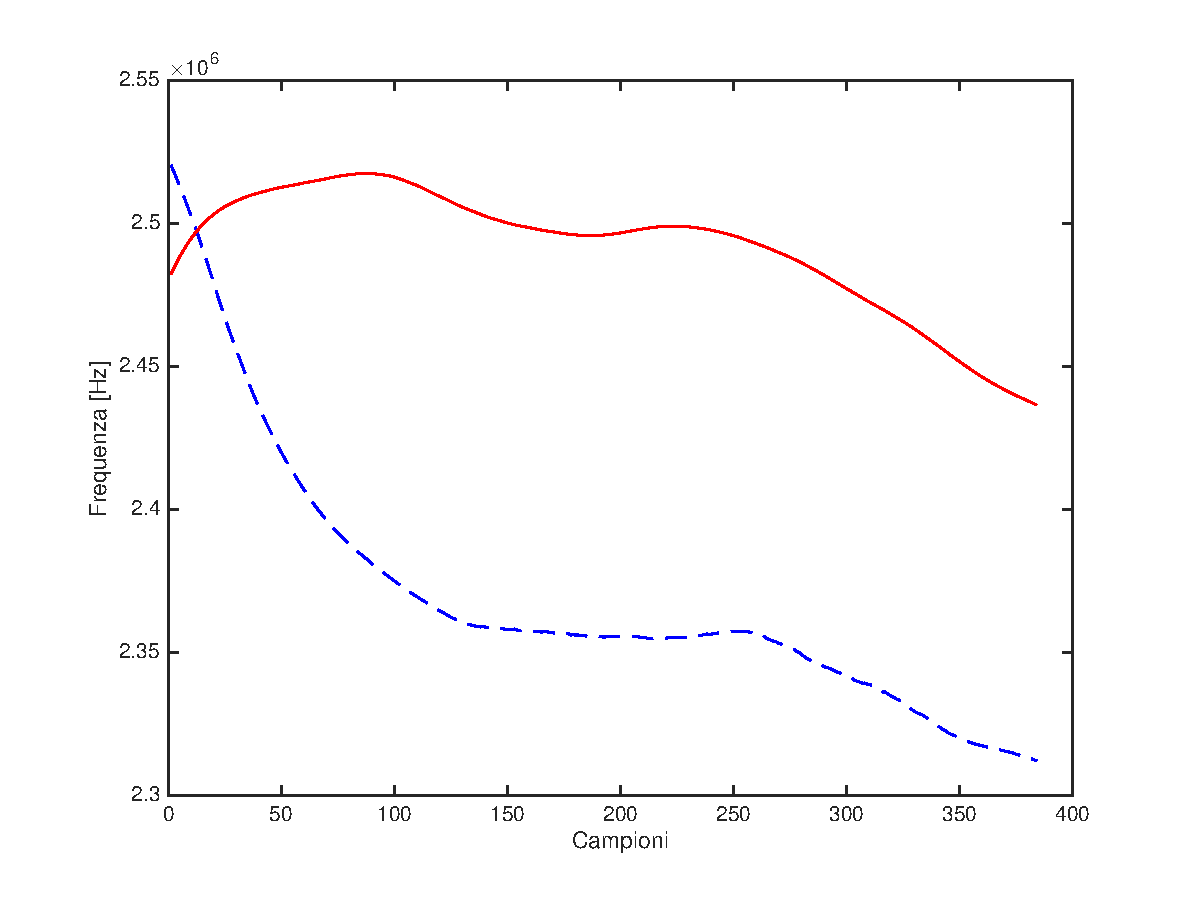
\includegraphics[scale=.6]{cap5/primadopocompdiscnew}}
\end{figure}
\begin{figure}[H]
	\centering
	\subfigure[Semiperiodo di salita]
	{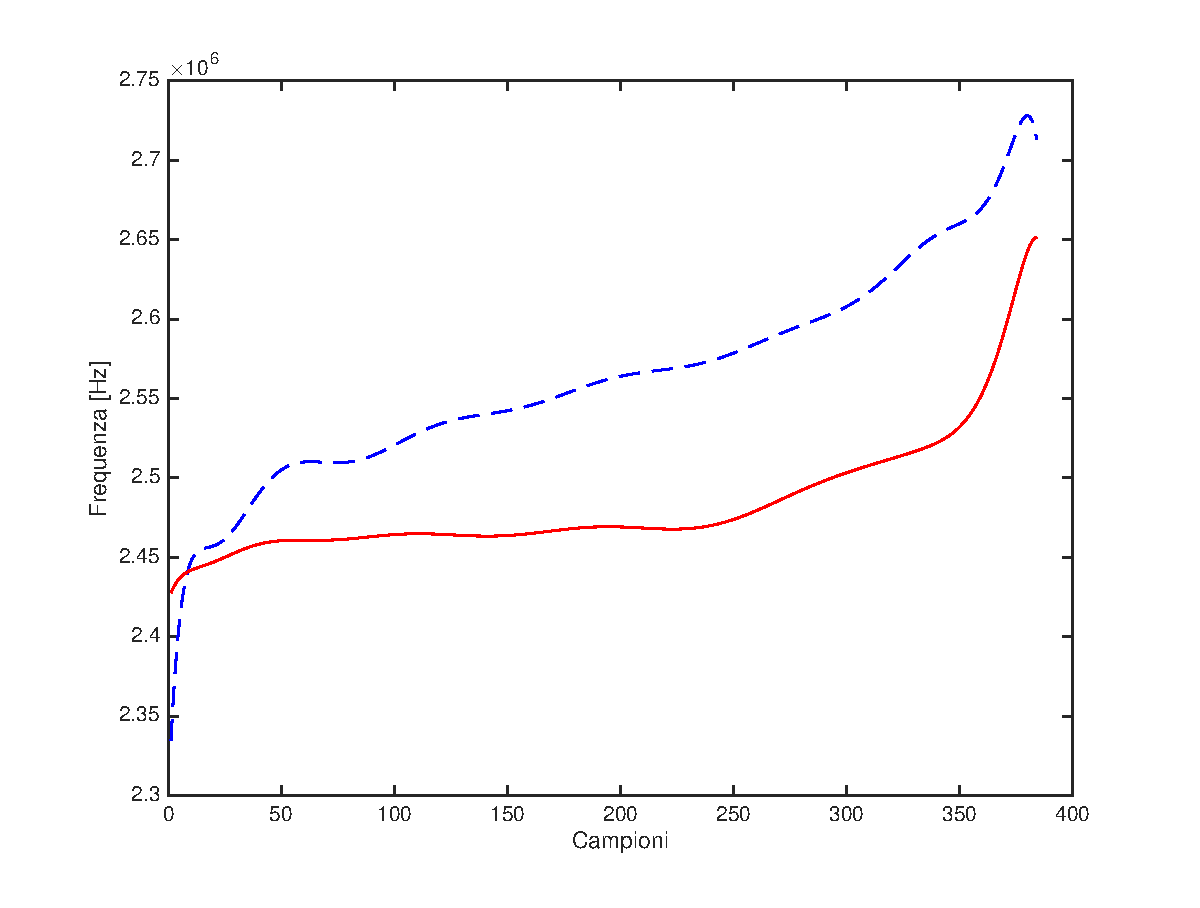
\includegraphics[scale=.6]{cap5/primadopocompsalnew}}
	\caption{Curve mediate delle frequenze estratte per entrambi i fronti di modulazione, con forma d'onda liscia (rosso) e non (blu)}\label{primadopocompnew}
\end{figure}
Con lo scopo di mostrare i miglioramenti ottenuti dell'algoritmo di compensazione ottimizzato, sono state comparate le curve delle frequenze ricavate con le due diverse forme d'onda. I miglioramenti sono mostrati in Figura \ref{primadopocompnew}. Dalle prove sperimentali è emerso che la massima variazione relativa di frequenza, valutata su $100$ semiperiodi di modulazione, è scesa intorno al $3\%$, per il semiperiodo di discesa, e $9\%$, per il semiperiodo di salita, contro i $9\%$ e $18\%$ ottenuti con la forma d'onda non liscia.
Nonostante il miglioramento nella linearità della frequenza di frangia, la nuova forma d'onda non ha apportato migliorie significative sulla precisione e l'accuratezza della misura. Per dimostrare quanto affermato, sono state effettuate le consuete prove ad ostacolo fisso e mobile i cui risultati sono riportati in Figura \ref{fissomodliscio} e \ref{mobilemodliscio}.

\begin{figure}[H]
	\centering
	\subfigure[Misure di distanza e media]
	{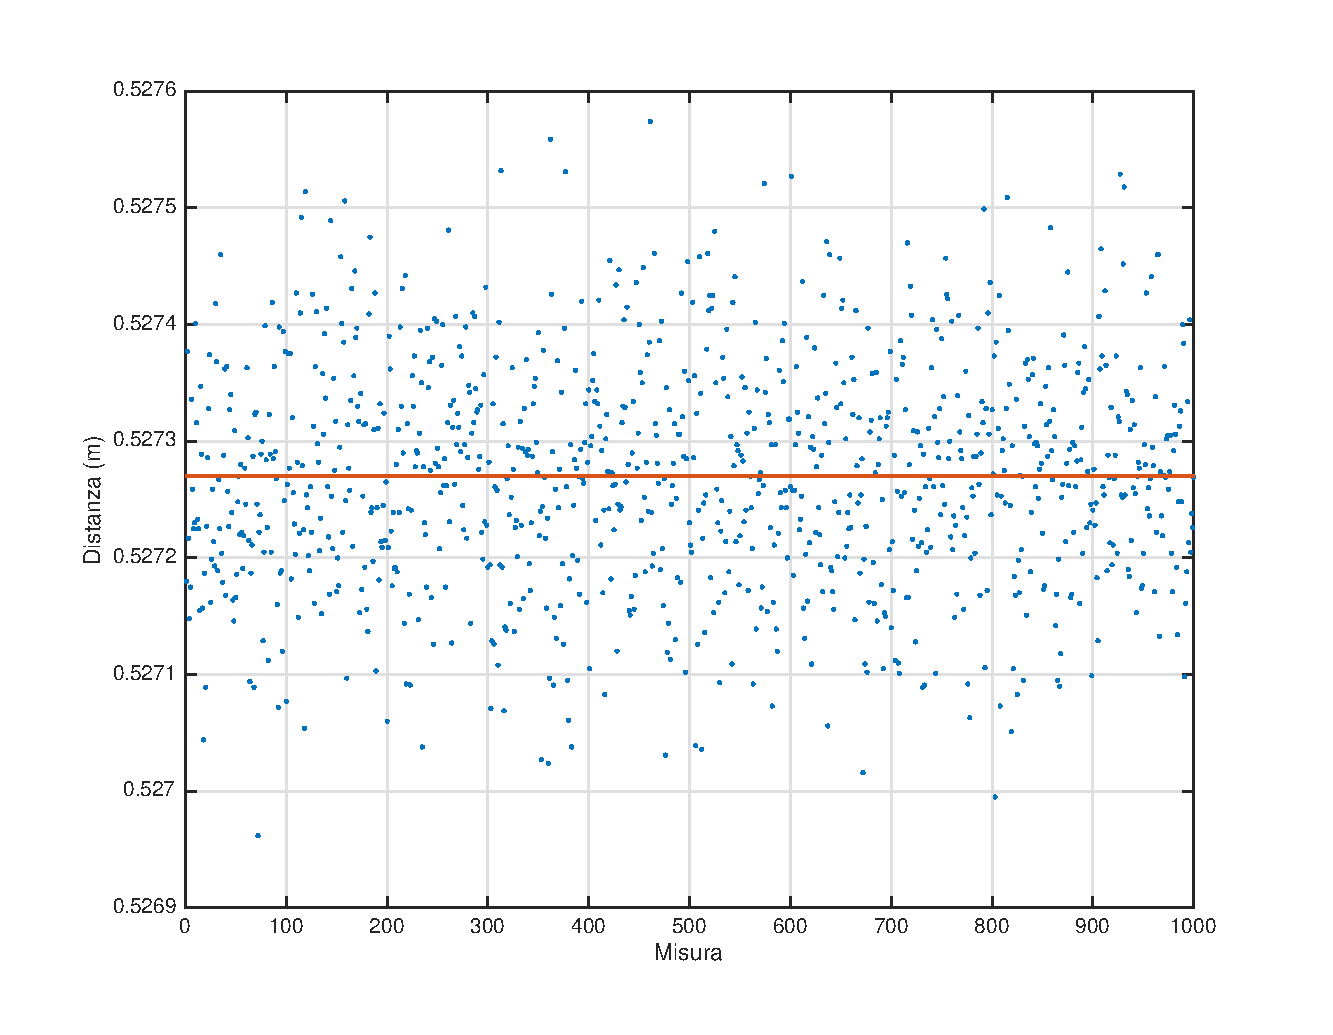
\includegraphics[scale=.5]{cap5/fissomodliscioa}}\end{figure}
\begin{figure}[H]
	\centering
	\subfigure[Distribuzione dei valori misurati rispetto alla media]
	{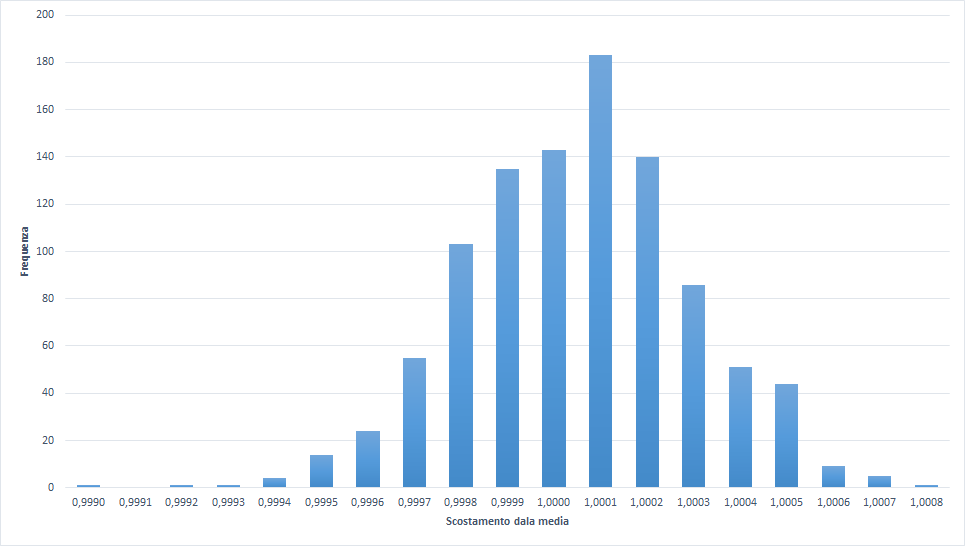
\includegraphics[scale=.6]{cap5/fissomodlisciob}}
	\caption{Misure di distanza a bersaglio fisso con segnale di modulazione compensato e liscio}\label{fissomodliscio}
\end{figure}
\begin{figure}[H]
	\centering
		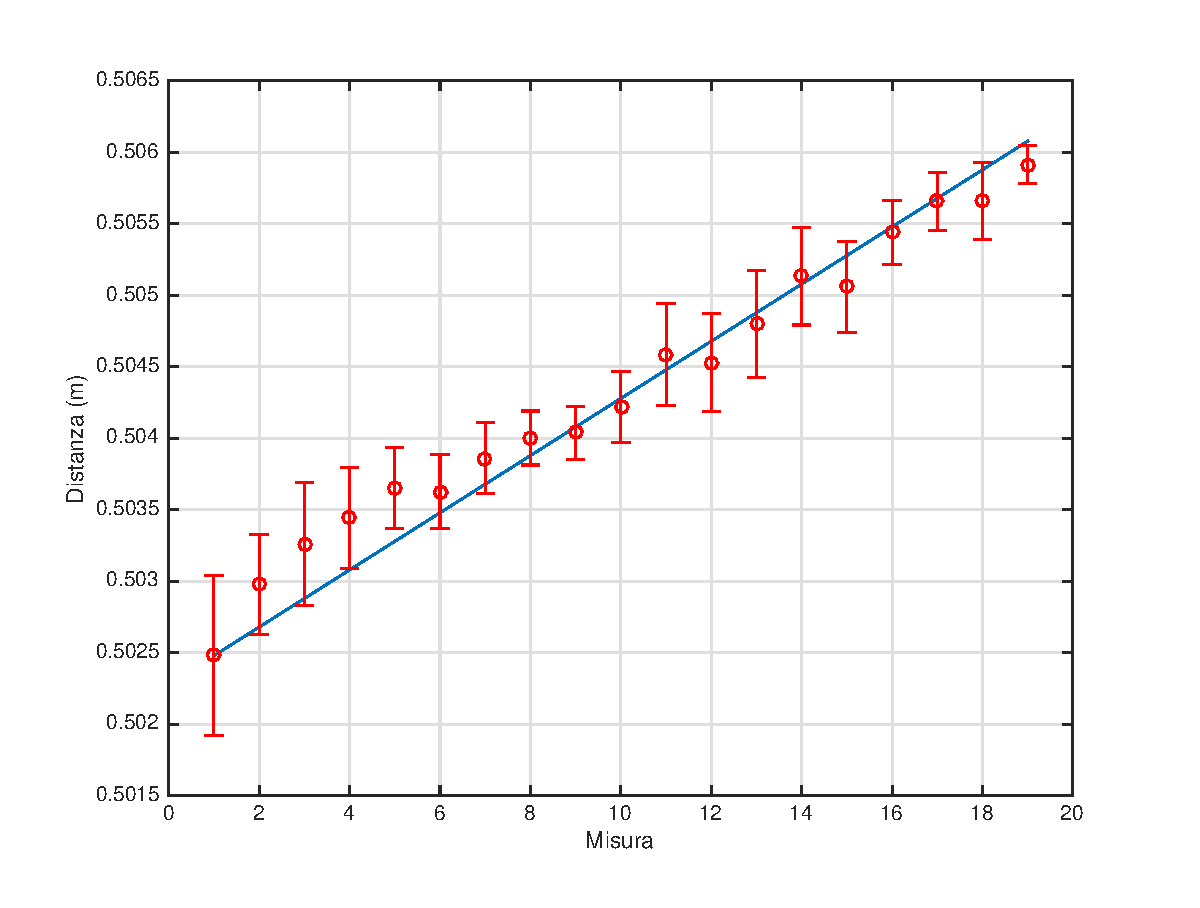
\includegraphics[scale=0.5]{cap5/mobilemodliscio}
		\caption{Misure di distanza a $50cm$ con bersaglio mobile effettuate su $200 \mu m$ di spostamento}
		\label{mobilemodliscio}
\end{figure}

\section{Drift termico}
Dal grafico in Figura \ref{mismobile5} è possibile notare, nonostante i buoni valori di errore picco-picco e RMS, una progressiva perdita di linearità della misura. In particolare le misure effettuate fino alla dodicesima possono essere considerate appartenenti alla retta ideale, mentre i successivi punti si discostano leggermente.

Un fenomeno simile è visibile anche nella prova a bersaglio fisso effettuata a $90cm$, dove si può notare un secondo picco nella distribuzione delle misure (Figura \ref{misfisso5b90}).

Questi fenomeni possono essere ricondotti a fenomeni termici del laser, che, non essendo termostatato, modifica la sua temperatura di funzionamento durante la prova. Inoltre, le condizioni ambientali non sono stabili durante lo svolgimento della prova, e una modifica della temperatura del laser può anche essere dettata da una variazione della temperatura ambientale.

Come accennato all'inizio del capitolo, per mitigare l'effetto del drift termico si lascia accesso e modulato il laser per un fissato periodo di tempo prima di utilizzarlo al fine di far raggiungere al laser una temperatura pressoché costante.



\section{Precisazione sui risultati ottenuti}
A causa della mole di dati presentata è necessario introdurre alcuni chiarimenti riguardanti i risultati ottenuti.

Innanzitutto è fondamentale considerare le condizioni di svolgimento della prova. Nonostante si siano prese tutte le dovute precauzioni per minimizzare le vibrazioni presenti su strumento e bersaglio non è stato possibile annullarle completamente. Questo, unito alla sensibilità dello strumento, porta la deviazione standard a non restare costante nel tempo, ma può avere degli scostamenti tra prove differenti. Inoltre questo stimatore dipende anche dal numero di campioni utilizzati per ricavarlo. 

Questa precisazione è necessaria in quanto alcuni risultati basati sulla deviazione standard possono apparire inconsistenti, come ad esempio il contrasto tra i risultati a bersaglio fisso e la prova del range di misura. La prima prova è stata effettuata mediando $1000$ acquisizioni, mentre la seconda è stata effettuata utilizzando soltanto $100$ campioni, il che porta ad un aumento della deviazione standard della misura. 

Per questa ragione, inoltre, non è possibile confrontare i risultati percentuali rispetto all'errore picco-picco e l'RMS della prova a bersaglio mobile con la deviazione standard registrata nella prova a bersaglio fisso, in quanto nella prova a bersaglio mobile sono stati mediati $100$ campioni, mentre in quella a bersaglio fisso $1000$.

Inoltre le misure sono state effettuate senza tener conto delle condizioni di temperatura dello strumento. Una variazione della temperatura di esercizio del laser può portare ad una differente precisione della misura e questo fatto può essere ulteriore causa di apparente inconsistenza tra i vari risultati presentati.

Concludendo, ogni prova descritta in questo Capitolo è stata rieseguita più volte e in istanti differenti al fine di validare la correttezza dei dati sperimentali ottenuti.
